% +--------------------------------------------------------------------+
% | LaTeX Template                                                     |
% | for K-State Electronic Theses, Dissertations, and Reports          |
% |                                                                    |
% | Comments and guidelines for using the template are shown           |
% | within boxes like this one.                                        |
% |                                                                    |
% | Revised 6/30/06                                                    |
% | 9/14/06: Removed typos                                             |
% +--------------------------------------------------------------------+

% +--------------------------------------------------------------------+
% | Your paper should contain the following sections, except where     |
% | indicated as optional, in the order shown.  Also, all headings     |
% | shown with an asterisk (*) must be centered and in uppercase       |
% | letters:                                                           |
% |                                                                    |
% | Abstract Title Page (doctoral dissertations only)                  |
% | ABSTRACT* (doctoral dissertations only)                            |
% | Title Page                                                         |
% | Copyright Page (Optional - only needed if copyrighting)            |
% | ABSTRACT *                                                         |
% | TABLE OF CONTENTS *                                                |
% | LIST OF FIGURES *                                                  |
% | LIST OF TABLES*                                                    |
% | ACKNOWLEDGMENTS* (Optional)                                        |
% | DEDICATION * (Optional)                                            |
% | PREFACE * (Optional)                                               |
% | Individual Chapters                                                |
% | References and/or bibliography                                     |
% | Appendices (as needed)                                             |
% +--------------------------------------------------------------------+

% +--------------------------------------------------------------------+
% | The LaTex keyword \documentclass selects a particular class to     |
% | associate with the document.  The current documentclass            |
% | {class_diss} generates a Table of Contents that has leading dots   |
% | only on chapter subheadings.  If you prefer a Table of Contents    |
% | that has leading dots for all entries, replace {class_diss}        |
% | with {Mydiss} in the command below.                                |
% |                                                                    |
% +--------------------------------------------------------------------+

\documentclass[final, 12pt,oneside]{class_diss}

% +--------------------------------------------------------------------+
% | The following command sets the bibliography style to American
% | Institute of Physics (AIP).  Other styles are available in the
% | styles directory.  To use a different style, replace "aip" with
% | the filename of the style you want to use.
% +--------------------------------------------------------------------+

\bibliographystyle{styles/plain}

\usepackage[utf8]{inputenc}
\usepackage{float}
\usepackage[T1]{fontenc}
\usepackage[spanish]{babel}
\usepackage[utf8]{inputenc}

% +--------------------------------------------------------------------+
% | Now, we add in all external packages that we will use throughout   |
% | the document.  You can add other packages as needed.
% +--------------------------------------------------------------------+

%\usepackage{     caption2} % Customize captions a bit more
\usepackage{      amsmath} % American Mathematics Society standards
%\usepackage{      wrapfig} % Wraps text around a figure or table
\usepackage{     graphicx} % Extended graphics package.
%\usepackage{     fancyhdr} % Efficiently handles headers and footers
%\usepackage{       braket} % Bra-Ket notation package
%\usepackage{     mathrsfs} % Specialized Math fonts (Hamiltonian, etc.)
%\usepackage{boxedminipage} % Boxed text can be produced
%\usepackage{     setspace} % Controls line spacing via \begin{space}

\usepackage{amsxtra}
\usepackage{amssymb}
\usepackage{amsthm}
\usepackage{latexsym}

\usepackage{listings} % For code display
\lstset{basicstyle=\ttfamily,
  showstringspaces=false,
  commentstyle=\color{red},
  keywordstyle=\color{blue}
}

% +--------------------------------------------------------------------+
% | The color package allows one to select colors for hyperlinking     |
% | (see below).                                                       |
% +--------------------------------------------------------------------+

\usepackage[usenames]{color}

% +--------------------------------------------------------------------+
% | Colors defined for use with this template.                         |
% +--------------------------------------------------------------------+

\definecolor{  Pink}{rgb}{1.0, 0.5, 0.5}
\definecolor{Maroon}{rgb}{0.8, 0.0, 0.0}

% +--------------------------------------------------------------------+
% | In the commands below, we use the 'natbib' package, and specify    |
% | the 'sort&compress' option, which condenses                        |
% | citations from (1,2,3,5,9,10,11) to (1-3,5,9-11).  The 'bibpunct'  |
% | option selects various parameters for how the citation will be     |
% | displayed.  In this case, only the comma (separation between       |
% | citations) and the 's' (superscript) arguments are chosen.  The    |
% | other curly braces deal with how to 'wrap' the citation (using     |
% | parentheses, brackets, etc.) and are not needed for the chosen     |
% | style.                                                             |
% +--------------------------------------------------------------------+

\usepackage[sort&compress]{natbib}
\bibpunct{}{}{,}{s}{}{}

% +--------------------------------------------------------------------+
% | Lastly, the hyperref package allows one to hyperlink cross-        |
% | references and figures in a LaTeX document.                        |
% +--------------------------------------------------------------------+

\usepackage[pdftex, plainpages=false, pdfpagelabels]{hyperref}

\hypersetup{
    linktocpage=true,
    colorlinks=true,
    bookmarks=true,
    citecolor=blue,
    urlcolor=red,
    linkcolor=Maroon,
    citebordercolor={1 0 0},
    urlbordercolor={1 0 0},
    linkbordercolor={.7 .8 .8},
    breaklinks=true,
    pdfpagelabels=true,
    }

% +--------------------------------------------------------------------+
% | Page margins are set on 1 inch on all sides.                       |
% +--------------------------------------------------------------------+

\topmargin      = -0.56in
\textheight     =  8.60in
\textwidth      =  6.46in
\oddsidemargin  =  0.02in

% +--------------------------------------------------------------------+
% | The document finally begins here.                                  |
% +--------------------------------------------------------------------+

\begin{document}


  \setcounter{page}{-1}


% +--------------------------------------------------------------------+
% | Title Page -- Required for both Doctoral and Masters Students
% +--------------------------------------------------------------------+

% +--------------------------------------------------------------------+
% | Title Page
% +--------------------------------------------------------------------+

\newpage

% +--------------------------------------------------------------------+
% | This page should not contain a page number.  We use the
% | \thispagestyle[empty] command below to suppress page numbers
% | and other style elements.
% +--------------------------------------------------------------------+

\thispagestyle{empty}

% +--------------------------------------------------------------------+
% | The Title page begins here.
% +--------------------------------------------------------------------+

\begin{center}

   \vspace{1cm}

% +--------------------------------------------------------------------+
% | On the line below, replace "ENTER YOUR TITLE" with the title of
% | your ETDR.  Use all CAPITAL LETTERS.
% +--------------------------------------------------------------------+

   {\Large EXPLICACIONES MEDIANTE REALIDAD AUMENTADA DE SISTEMAS DE RECOMENDACIÓN SOCIAL EN EL DOMINIO DEL OCIO}\\

   \vspace{0.5cm}



   \vspace{0.5cm}



    Diego Acuña Berger, Daniel Calle Sánchez, Carlos Gómez Cereceda, Zihao Hong\\

   \vspace{0.5cm}




   GRADO EN INGENIERÍA DEL SOFTWARE. FACULTAD DE INFORMÁTICA\\
   UNIVERSIDAD COMPLUTENSE DE MADRID \\


   \vspace{0.65cm}
   \rule{2in}{0.5pt}\\
   \vspace{0.85cm}

  
\includegraphics[height=2.5in]{figures/escudo.jpg}
  

%+-- Escribe el nombre de tu asignatura de fin de master (Ingeniería de computadores,....)
   \vspace{0.5cm}
Trabajo Fin de Grado en Ingeniería del Software

   \vspace{0.5cm}





% +--------------------------------------------------------------------+
%  Fecha 
% +--------------------------------------------------------------------+

  Fecha\\
  CURSO 2018-2019
   \vspace{1cm}

\end{center}

{\raggedleft
Director/es y/o colaborador:\\
   \vspace{ 1cm}
Juan Antonio Recio García\\
Guillermo Jiménez Díaz\\
}


% +--------------------------------------------------------------------+
% | Use the section below if you have co-major professors.
% +--------------------------------------------------------------------+

%\begin{flushleft}
%   \hspace{10cm}Approved by:\\
%   \vspace{ 1cm}
%   \hspace{10cm}Co-Major Professor\\
%   \hspace{10cm}Enter Your Co-Major Professor's Name\\
%   \vspace{.5cm}
%   \hspace{10cm}Co-Major Professor\\
%   \hspace{10cm}Enter Your Co-Major Professor's Name\\
%\end{flushleft}

   \pdfbookmark[0]{Portada}{PDFPortadaPage}

% +--------------------------------------------------------------------+
% | Autorizacion Page -- Required for both Doctoral and Masters Students
% +--------------------------------------------------------------------+

% +--------------------------------------------------------------------+
% | Copyright Page
% +--------------------------------------------------------------------+

\newpage

\thispagestyle{empty}

\begin{center}

{\bf \Huge Autorización de difusión}

\vspace{1cm}

% +--------------------------------------------------------------------+
% | On the line below, replace "Enter Your Name" with your name
% | Use the same form of your name as it appears on your title page.
% | Use mixed case, for example, Lori Goetsch.
% +--------------------------------------------------------------------+

     Diego Acuña Berger, Daniel Calle Sánchez, Carlos Gómez Cereceda, Zihao Hong\\

   \vspace{0.5cm}

% +--------------------------------------------------------------------+
% | On the line below, replace Fecha
% |
% +--------------------------------------------------------------------+

   Fecha\\

   \vspace{0.5cm}
   \end{center}
   
Los abajo firmantes, matriculados en el Grado en Ingeniería del Software de la Facultad de Informática, autoriza a la Universidad Complutense de Madrid (UCM) a difundir y utilizar con fines académicos, no comerciales y mencionando expresamente a sus autores el presente Trabajo Fin de Grado: “EXPLICACIONES MEDIANTE RA DE SISTEMAS DE RECOMENDACIÓN SOCIAL EN EL DOMINIO DEL OCIO”, realizado durante el curso académico 2018-2019 bajo la dirección de Juan Antonio Recio García y Guillermo Jiménez Díaz en el Departamento de Ingeniería del Software e Inteligencia Artificial, y a la Biblioteca de la UCM a depositarlo en el Archivo Institucional E-Prints Complutense con el objeto de incrementar la difusión, uso e impacto del trabajo en Internet y garantizar su preservación y acceso a largo plazo.


   \pdfbookmark[0]{Autorización}{PDFAutorizacionPage}


   
   % +--------------------------------------------------------------------+
% | Copyright Page
% +--------------------------------------------------------------------+

\newpage

\thispagestyle{empty}

\begin{center}

{\bf \Huge Resumen en castellano}

  \end{center}
\vspace{1cm}

Hemos desarrollado una aplicación móvil con la que poder identificar
carteles de distintas películas para obtener información en tiempo real de
éstas mediante el uso de Realidad Aumentada, tales como su trailer o su valoración. Además,
se incluye la posibilidad de guardar esta información o incluir la película en un plan, para 
su posterior visualización según la recomendación que nos dé la aplicación en base a 
los gustos de los usuarios que están dentro del plan y las películas que se han añadido. 
También hemos realizado un pequeño ejemplo de reconocimiento facial de otros usuarios para observar, 
mediante Realidad Aumentada, información sobre sus gustos o películas vistas anteriormente.

\vspace{1cm}

% +--------------------------------------------------------------------+
% | On the line below, repla	ce Fecha
% |
% +--------------------------------------------------------------------+

\begin{center}

{\bf \Large Palabras clave}

   \end{center}

   \vspace{0.5cm}
   
   Lista de palabras clave
   



   
   \pdfbookmark[0]{Resumen}{PDFResumenPage}

    % +--------------------------------------------------------------------+
% | Copyright Page
% +--------------------------------------------------------------------+

\newpage

\thispagestyle{empty}

\begin{center}

{\bf \Huge Abstract}

  \end{center}
\vspace{1cm}

When the idea of this project was suggested we observed that, as it$'$s name indicates, the
domain of the project is leisure, in particular the world of cinema. It came up from the need of 
the people who wanted to watch a movie accompanied by someone, either by friends or by someone who has
a similar taste, being the affinity of people to certain film a relevant characteristic at the time of making
a decision to go see the movie. With this we want to reflect that anyone who has a certain degree of cinephilia could be interested
in our idea. Therefore, to answer this need we$'$ve developed a mobile application with which we can recognize movie
posters and images of user$'$s faces, to see related real time information and to be able to interact with it through 
Augmented Reality (AR). We will be able to create plans to go watch a movie with other users of the application and it 
will also recommend plans with a movie related to their tastes.

\vspace{1cm}

% +--------------------------------------------------------------------+
% | On the line below, replace Fecha
% |
% +--------------------------------------------------------------------+
\begin{center}

  {\bf \Large Keywords}
  
     \end{center}
  
     \vspace{0.5cm}
     
     Keywords list
     \begin{itemize}  
      \item Augmented Reality
      \item Recommendation Systems
      \item Unity
      \item Android
      \item Spring
      \item Vuforia
      \item PostgreSQL
      \item Java
      \item C\#
      \item Cloud
      \item Server
      \item API Rest
      \item Heroku
    \end{itemize}
   



       \pdfbookmark[0]{Abstract}{PDFAbstractPage}
    \vfill


% +--------------------------------------------------------------------+
% | We use the following code to suppress page numbers and other
% | style issues we do not want present on a given page.               |
% +--------------------------------------------------------------------+

%\thispagestyle{empty} Looks like it's ok to remove this line
\newpage
\pagenumbering{roman}

% +--------------------------------------------------------------------+
% | On the line below, set the number to represent the page number of
% | the Table of Contents page.  For example, if the Table of Contents
% | page is the 8th page of your document, enter 8 in the brackets.  This
% | number may vary, depending on the length of your abstract.
% |
% | Numbers do not appear on the title and abstract pages, but they are
% | included in the page count.  The Table of Contents page is the
% | first page on which page numbers are displayed.
% +--------------------------------------------------------------------+

\setcounter{page}{1}

% +--------------------------------------------------------------------+
% | Here, we will generate our Table of Contents (TOC) entries.        |
% | This adds the section to the TOC and then generates the indicated  |
% | section.                                                           |
% +--------------------------------------------------------------------+

\phantomsection
\addcontentsline{toc}{chapter}{Índice}

\tableofcontents
%\listoffigures
%\listoftables

%\hfill  Are these lines necessary?
%\hfill

% +--------------------------------------------------------------------+
% | Acknowledgements Page
% |
% | If you choose not to have an Acknowledgements page, comment out
% | or delete the following 3 lines.
% +--------------------------------------------------------------------+

% +--------------------------------------------------------------------+
% | Acknowledgements Page (Optional)                                   |
% +--------------------------------------------------------------------+

\newpage
\begin{center}
{\bf \Huge Agradecimientos}
\end{center}
\vspace{1cm}
\setlength{\baselineskip}{0.8cm}

%\pdfbookmark[0]{Acknowledgements}{PDF_Acknowledgements}

% +--------------------------------------------------------------------+
% | Enter text for your acknowledgements in the space below this box.  |
% |                                                                    |
% +--------------------------------------------------------------------+

Nos gustaría agradecer a nuestra familia y compañerxs la confianza depositada en nosotros así como la realimentación
recibida por parte de toda persona que se ha involucrado en mayor o menor medida en la realización de nuestro proyecto, ya 
fuera mediante comentarios constructivos o la redirección a la documentación de tecnologías que usaríamos posteriormente.

\phantomsection
\addcontentsline{toc}{chapter}{Agradecimientos}

% +--------------------------------------------------------------------+
% | Dedication Page
% |
% | If you choose not to have a Dedication page, comment out
% | or delete the following 3 lines.
% +--------------------------------------------------------------------+

% +--------------------------------------------------------------------+
% | Dedication Page (Optional)
% +--------------------------------------------------------------------+

\newpage
\begin{center}
{\bf \Huge Dedicatoria}
\end{center}
\vspace{1cm}
\setlength{\baselineskip}{0.8cm}

%\pdfbookmark[0]{Dedication}{PDF_Dedication}

% +--------------------------------------------------------------------+
% | Enter the text for your dedication in the space below this box.
% +----------------
Texto...
\phantomsection
\addcontentsline{toc}{chapter}{Dedicatoria}

% +--------------------------------------------------------------------+
% | Preface Page
% +--------------------------------------------------------------------+

%% +--------------------------------------------------------------------+
% | Preface (Optional)
% +--------------------------------------------------------------------+

\newpage
\begin{center}
{\bf \Huge Preface}
\end{center}
\vspace{1cm}
\setlength{\baselineskip}{0.8cm}

%\pdfbookmark[0]{Preface}{PDF_Preface}

% +--------------------------------------------------------------------+
% | Enter text of your Preface in the space below this box.
% +--------------------------------------------------------------------+

This template uses a separate file for each section of your ETDR:
title page, abstract, preface, chapters, reference, etc.  This
makes it easier to organize and work with a lengthy document.  The
template is configured with page margins required by the Graduate
School and will automatically create a table of contents, lists of
tables and figures, and PDF bookmarks.

Although the template gives you a foundation for creating your
ETDR, you will need a working knowledge of LaTeX in order to
produce a final document.  You should be familiar with LaTeX
commands for formatting text, equations, tables, and other
elements you will need to include in your ETDR.

This template uses a separate file for each section of your ETDR:
title page, abstract, preface, chapters, reference, etc.  This
makes it easier to organize and work with a lengthy document.  The
template is configured with page margins required by the Graduate
School and will automatically create a table of contents, lists of
tables and figures, and PDF bookmarks.

Although the template gives you a foundation for creating your
ETDR, you will need a working knowledge of LaTeX in order to
produce a final document.  You should be familiar with LaTeX
commands for formatting text, equations, tables, and other
elements you will need to include in your ETDR.

This template uses a separate file for each section of your ETDR:
title page, abstract, preface, chapters, reference, etc.  This
makes it easier to organize and work with a lengthy document.  The
template is configured with page margins required by the Graduate
School and will automatically create a table of contents, lists of
tables and figures, and PDF bookmarks.

Although the template gives you a foundation for creating your
ETDR, you will need a working knowledge of LaTeX in order to
produce a final document.  You should be familiar with LaTeX
commands for formatting text, equations, tables, and other
elements you will need to include in your ETDR.

%\phantomsection
%\addcontentsline{toc}{chapter}{Preface}

% +--------------------------------------------------------------------+
% | We use arabic (1, 2, 3...) page numbering starting from page 1.    |
% | Note, however, that there are many pages where this is not the     |
% | desired behavior - such as the Title page, or abstract.  In these  |
% | cases, we can use \thispagestyle{empty} to suppress page numbers,  |
% | and other general style issues that we've defined globally.        |
% +--------------------------------------------------------------------+

\newpage
\pagenumbering{arabic}
\setcounter{page}{1}

% +--------------------------------------------------------------------+
% | Here is where we include individual sections of the thesis or
% | dissertation.                                                      |
% +--------------------------------------------------------------------+

% +--------------------------------------------------------------------+
% | Chapters
% +--------------------------------------------------------------------+

% +--------------------------------------------------------------------+
% | Sample Chapter
% |
% | This file provides examples of how to
% | - insert a figure with a caption
% | - construct a table with a caption
% | - create subsections within the chapter
% | - insert a reference to a Figure or Table
% | - make a citation
% +--------------------------------------------------------------------+

\cleardoublepage

% +--------------------------------------------------------------------+
% | Replace "Chapter Title" below with the title of your chapter.  LaTeX
% | will automatically number the chapters.
% +--------------------------------------------------------------------+

\chapter{Introducción}
%\label{ch:chapter1}
\label{makereference}


    En este capítulo introduciremos la idea de nuestro proyecto, de dónde surge, qué objetivos queremos lograr y cómo nos hemos organizado a la hora de trabajar.
    Con este proyecto queremos desarrollar una aplicación para solventar una serie de situaciones en las que una persona
    tiene ganas de ver cierta película, ya sea porque se ha encontrado el cartel de la nueva película
    de su saga favorita anunciada en la calle y no sabe con quién ir, o porque quizás un amigo le ha sugerido que le acompañe
    a ver una película de la que no saben nada por el mero hecho de ir al cine. 
    Decidimos ponernos manos a la obra y desarrollar una aplicación móvil que permitiera a sus usuarios actuar en distintas situaciones
    para que con el simple uso de la cámara de su smartphone, e incluso sin ella, pudieran de forma
    fácil e interactiva, organizarse para ir al cine o a ver la película a casa de otra persona. Además, podrían apoyarse en la 
    información que la aplicación les proporciona sobre las distintas películas para decidir si les es interesante ir a verla, sobre todo 
    si es para ir al cine ya que el usuario podría ahorrarse el gasto de acabar viendo una película que no le gusta por no poder saber si se 
    ajusta a sus gustos. Además, tener una red de contactos de personas interesadas en ver películas que a ti también te gusten y tener la posibilidad
    de quedar en un lugar, fecha y hora determinados refuerzan el atractivo de nuestra aplicación en el dominio del ocio.
    Nuestro proyecto ofrecerá a los usuarios explicaciones sobre el objeto que se esté reconociendo mediante la realidad aumentada, es decir, al usuario se le 
    recomendarán productos relevantes de la aplicación según sus gustos, también se le mostrará información sobre los objetos que se reconocen.

% +--------------------------------------------------------------------+
% |To create cross-references to figures, tables and segments
% |of text, LaTeX provides the following commands:
% |   \label{marker}
% |   \ref{marker}
% |   \pageref{marker}
% | where {marker} is a unique identifier.
% |
% | In the line above, we use \label{figure1} to mark a location
% | we wish to refer to later.  LATEX replaces \ref by the number of
% | the chapter, section, subsection, figure, or table after which the
% | corresponding \label command was issued. \pageref prints the page
% | number of the page where the \label command occurred.
% |
% +--------------------------------------------------------------------+


% +--------------------------------------------------------------------+
% | Replace \section headings below with the title of your
% | subsections.  LaTeX will automatically number the subsections 1.1,
% | 1.2, 1.3, etc.
% +--------------------------------------------------------------------+

\section{Antecedentes}
\label{makereference1.1}

Para entender de donde surge nuestra idea tenemos que remontarnos al momento en el que se propuso este proyecto.
El principal motivo es la mejora de un Trabajo de Fin de Grado anterior
 al nuestro\cite{TFGRA16}, cuyo enfoque y finalidad era el mismo. Nuestro objetivo principal es 
 ampliar su funcionalidad diferenciándonos, sobre todo, en las tecnologías usadas y 
 en los casos de uso representados.

 En nuestra aplicación no solo nos centramos en ir al cine y reconocer películas que estuvieran en la cartelera
 para que nos recomiende la que más se ajuste a nuestros gustos. Decidimos que el usuario podría crear planes con
 una película que le interesase ver y que sus amigos u otros usuarios pudieran unirse para ir todos juntos a verla.
 También añadiremos más interacción sobre las escenas de realidad aumentada, permitiéndonos ver la información sobre la 
 película reconocida, ver trailers o guardarla en la lista de favoritos. Además, con la realidad aumentada,
 se podrán realizar reconocimientos faciales sobre los usuarios para añadirlos como amigos, para después recomendarnos en tiempo real
 que películas podemos ir a ver con éstos.

\section{Objetivos}
\label{makereference1.2}
Nuestro objetivo principal es crear una aplicación que ayude a los usuarios a
realizar planes con sus amigos para ir al cine a ver películas. Además,
mostrará qué películas pueden interesar al usuario en base a sus gustos.
También se usarán tecnologías de realidad aumentada que ayuden al usuario a usar
la aplicación.
La lista de subobjetivos es la siguiente:
\begin{itemize}  
    \item Estudiar las tecnologías de realidad aumentada actuales.
    \item Analizar sistemas de recomendación, así como su uso dentro del
     proyecto.
    \item Definir casos de uso reales que aporten valor a la aplicación.
    \item Diseñar una aplicación para dispositivos móviles que aplique las
     anteriores tecnologías.
    \item Diseñar y aplicar una arquitectura que cumpla las necesidades del
     proyecto.
\end{itemize}

\section{Plan de trabajo}
\label{makereference1.3}

Para comenzar con nuestro proyecto analizaremos el estado del arte, en el
 \autoref{makereference2}, en el que estudiaremos los conceptos básicos de la
 Realidad Aumentada y buscaremos las tecnologías actuales a la fecha del proyecto
 que funcionen en dispositivos móviles. También realizaremos un estudio de las distintas
 fuentes de información de las que podemos obtener datos y un estudio de
 técnicas de recomendación.

Después realizaremos las tareas de diseño, descritas en el
 \autoref{makereference3}. Primero, un análisis de aquellas aplicaciones que se
 asemejen a nuestra idea. A continuación, nos plantearemos los distintos
 escenarios en los que sería usada nuestra aplicación. Posteriormente
 realizaremos una lista de las funcionalidades más importantes de nuestra
 aplicación y diseñaremos las interfaces de usuario que acompañarán a dichas
 funcionalidades. 
   
El siguiente paso, descrito en el \autoref{makereference4}, comenzará con
 el desarrollo de una serie de prototipos con distintas tecnologías que nos permitan
 decidir cuales utilizar en la implementación de la aplicación final. Después diseñaremos la
 arquitectura e implementaremos la aplicación, para lo cual aplicaremos algunas
 prácticas de la metodología SCRUM. El desarrollo se realizará con iteraciones
 cercanas a las dos semanas. Comenzará con la selección de objetivos más
 prioritarios y terminará con las reuniones de revisión junto con los directores
 del Trabajo de Fin de Grado. Tras cada iteración, los miembros del equipo
 realizaremos una reunión de retrospectiva para identificar en qué hemos fallado
 durante esta iteración y cómo podemos mejorar para la siguiente.

Finalmente en el \autoref{makereference5}, hablaremos de las conclusiones que
 hemos obtenido tras realizar el proyecto, seguido del trabajo futuro que se podría realizar sobre nuestra
 aplicación para conseguir futuras mejoras en el \autoref{makereference5.2}.

\section{Introduction}

In this chapter we are going to introduce the idea of our project, where it comes from,
 what objectives we want to achieve and how we have organized ourselves to work 
together. With this project we want to develop an application to solve a series 
of situations in which a person wants to watch a certain movie, either because he 
has encountered the poster of a new movie of it$'$s favorite saga announced on the 
street and doesn$'$t know who to go with, or because maybe a friend of him has 
suggested on going to see a movie together they don$'$t know about 
by the mere fact of going to the cinema. We decided to get to work and develop a 
mobile application that would allow it$'$s users to act in different situations so 
that with the simple use of their smarthpone$'$s camera, or even without it, 
they could get organized to go to the cinema or to watch the movie in another 
person$'$s house in an easy and interactive way. Also, they could rely on 
the information that the application provides them about the different movies so they can decide 
whether to watch it or not, especially if it is for going to the cinema since the user could save himself 
the expense of ending up watching a movie thath he doesn$'$t like because he can$'$t know if it fits 
his tastes. Furthermore, having a network of contacts of people interested in going to watch films that
you like too and having the possibility of meeting on a certain place, date and hour will reinforce the attractive
of our application in leisure$'$s domain.

\section{Background}

To understand where our idea comes from we have to go back to the moment in which this project was proposed.
The main reason is the improvement of a Final Degree Project previous to ours \cite{TFGRA16}, which approach and purpose was the same. Our main 
objective is to extend it$'$s functionality differentiating us, especially, in the technologies used and in the represented use cases.

In our application we don$'$t just focus on going to the cinema and recognizing films that were 
on the billboard so that it can recommend us the movie that fits our tastes better. We decided that an user
could create plans with a film he is interested in watching and that his friends or other users could join so they can
all go together. We will also add more interaction to the augmented reality scenes, allowing us to see the information about
the film we are recognizing, watch trailers or save it to our favorites list. Furthermore, with augmented
reality, it will be possible to realize facial recognitions of users so we can add them as friends, so it can afterwards recommends us
films that we can go watch with them in real time.

\section{Objectives}

Our main objective is to create an application that will help the users to carry out plans with their friends to go
to the cinema to watch movies. It will also show what films are interesting for the user based on his tastes. We will also use
augmented reality technologies that will help the user to use the application. The list of subobjectives is the next one:

\begin{itemize}
    \item Study the current augmented reality technologies.
    \item Analize recommendation systems, as well as it$'$s use inside the project.
    \item Define real uses cases that will add value to the application.
    \item Design an application for mobile devices that will apply the technologies described before.
    \item Design and apply an architecture that meets the needs of the project.
\end{itemize}

\section{Workplan}

To start with our project we will analize the state of art, in Chapter 2, in which we will
study the basic concepts of augmented reality and we will search the current technologies to the project$'$s date that
work in mobile devices. We will also perform a study of the different information sources from which we can obtain data and we will
also perform a study about recommendation techniques.

Afterwards we will perform design tasks, described in Chapter 3. First, an analysis of those 
applications which are similar to our idea. Then, we will consider the different scenarios in which
our application will be used. Later we will do a list of the most important functionalities of our application 
and design the user interfaces that will accompany these functionalities.

The next step, described in Chapter 4, will start with the development of a series of prototypes with different
technologies that will allow us to decide which ones to use in the implementation of our final application. After we 
will design the architectura and implement the application, for it we will apply some practices of the SCRUM methodology. 
The development will be carried out with iterations close to the two weeks of duration. It will start with the selection 
of the most priority objectives and will end with review meetings alongside the Final Degree Project directors. After each iteration,
all of the team members will attend a retrospective meeting to identify in what we have failed during this iteration and 
how we could improve for the next one. 

Finally in Chapter 5, we will speak about the conclusions we have obtained from implementing this project, followed by the future work that
could be done in our application tu achieve future improvements in Section 5.2.


% +--------------------------------------------------------------------+
% | Uncomment the lines below to add additional chapters.  Name the
% | files chapter2.tex for Chapter 2, chapter3.tex for Chapter 3, etc.
% +--------------------------------------------------------------------+

% +--------------------------------------------------------------------+
% | Sample Chapter 2
% +--------------------------------------------------------------------+

\cleardoublepage

% +--------------------------------------------------------------------+
% | Replace "This is Chapter 2" below with the title of your chapter.
% | LaTeX will automatically number the chapters.
% +--------------------------------------------------------------------+

\chapter{Estado del arte}
\label{makereference2}
En esta sección de la memoria procederemos a describir las tecnologías que hemos implementado
en nuestro trabajo, tales como la \textbf{realidad aumentada}, las distintas \textbf{fuentes de información}, 
\textbf{técnicas de recomendación}, junto a un análisis de la \textbf{competencia}.
\section{Realidad Aumentada}
\label{makereference2.1}
Según el enlace de Wikipedia: \url{https://es.wikipedia.org/wiki/Realidad_aumentada}, la \textbf{realidad aumentada} es el término que se 
usa para describir al conjunto de tecnologías que permiten que un usuario visualice parte de mundo real a través de un dispositivo tecnológico 
con información gráfica añadida por éste dispositivo. Este dispositivo o conjunto de dispositivos, añaden información virtual a la información 
física ya existente; es decir, una parte sintética virtual a la real. Podemos estar de acuerdo en que es una tecnología en auge actualmente, sobre todo 
en el uso de los \textbf{smartphones} ya que prácticamente todas las personas poseen uno. Esta tecnología nos permite añadir un valor importante a 
nuestra aplicación, por lo que consideramos que el grueso de nuestro proyecto se centra en ella. Los casos de uso más importantes de nuestra aplicación 
usarán la \textbf{realidad aumentada} para proveer al usuario de información adicional y de gran relevancia de las imágenes que reconozca, ya sean carteles
de películas o caras de usuarios que usen la aplicación.
\subsection{Tecnologías actuales}
\label{makereference2.1.1}
\paragraph{ARCore:}
Plataforma creada por Google para desarrollar aplicaciones de
 realidad aumentada con soporte para Android, Android NDK, iOS,
 Unity y Unreal Engine. Aunque las funcionalidades que se ofrecen
 para iOS y Unity for iOS se limitan a Cloud Anchors, los anchors
 sirven para hacer que objetos virtuales aparezcan en un lugar
 captado por la cámara de nuestro dispositivo estos son compartidos
 en la nube para que multitud de dispositivos disfruten de la misma
 experiencia, los dispositivos con iOS podrán usarlos utilizando ARKit.

Tiene una curva de aprendizaje media y con su versión 1.5 demuestra una
 estabilidad interesante respecto a su reciente creación. Cabe destacar
 que no todos los dispositivos son compatibles, esto depende de que las
 empresas que desarrollan estos dispositivos cumplan unos requisitos
 para asegurar que la experiencia con ARCore es la adecuada y de la
 versión del sistema operativo. se puede ver con más detalle en esta
 dirección \url{https://developers.google.com/ar/discover/supported-devices}.

ARCore usa tres características a través de la cámara del dispositivo:
 \begin{itemize}  
     \item {\bf Motion tracking} permite al dispositivo entender y rastrear la posición relativa del mundo.
     \item {\bf Environmental understanding} permite al dispositivo detectar el tamaño y localización de todos los tipos de superficies.
     \item {\bf Light estimation} permite al dispositivo estimar las condiciones de luz del entorno actual.
 \end{itemize}

\paragraph{ARKit:}
Podemos utilizar experiencias de realidad aumentada persistente, compartirlas entre distintos dispositivos iOS,
 detecta imágenes 2D incluso en movimiento y objetos 3D.

\paragraph{Wikitude:}
Kit de desarrollo para realidad aumentada con soporte para Android, iOS, Unity, Cordova, Xamarin (mala
 documentación y versiones obsoletas), Titanium, React Native.
Su licencia es de pago, aunque hay versiones limitadas gratuitas.
Utiliza ARCore o ARKit cuando los dispositivos lo soportan y en caso de que no utiliza tecnología de Wikitude
 para que el número de dispositivos compatibles sea mayor. 

\paragraph{Vuforia:}
Kit de desarrollo para realidad aumentada con soporte para Android, iOS, UWP y Unity.
Software de pago solo permite usarse gratis para pruebas.

\paragraph{ViroReact:}
Plataforma para construir aplicaciones con realidad aumentada usando React Native.
 Utiliza ARKit y ARCore para dotar a las aplicaciones de una experiencia de RA sin
 utilizar código distinto y con una curva de aprendizaje fácil. Al basarse en React
 Native que no tiene versión estable provoca problemas con las versiones de dependencias,
 configuraciones tediosas y largas compilaciones.
Es un software privativo gratuito.

\paragraph{Expo AR:}
API que permite crear aplicaciones en React Native utilizando ARKit únicamente.
Está en una fase muy inicial.

\section{Análisis de la competencia}
\label{makereference2.2}
\begin{flushleft}
    Consideramos que la aplicación que hemos diseñado consta de dos partes claramente diferenciadas (la parte de \textbf{Realidad Aumentada} 
    y la parte de \textbf{Recomendación y gestión} de películas), consideramos que existen distintos tipos de competencia dependiendo de cada una de ellas.
     \begin{itemize}  
         \item En la parte de recomendación y gestión de películas, compite claramente con aplicaciones como \textbf{IMDB} o \textbf{MovieBase}. 
         Estas aplicaciones proporcionan, herramientas para guardar películas y recomendar éstas a los usuarios en función de sus gustos. Estas funcionalidades son 
         muy parecidas a las que nosotros hemos decidido proporcionar a nuestros usuarios, con la diferencia que nuestra aplicación, además de las funcionalidades anteriormente 
         mencionadas, permite realizar más acciones sobre las películas como crear planes con amigos.
        \item A diferencia de la parte de recomendación y gestión en donde hay una gran variedad de aplicaciones que ofrecen servicios parecidos a los nuestros, únicamente hemos 
        encontrado una aplicación (\textbf{Paramount AR+}) que ofrezca servicios parecidos a los nuestros relacionados con Realidad Aumentada. Según las especificaciones de la aplicación permite identificar pósteres y 
        mostrar información sobre la película detectada, servicio muy parecido al que nosotros hemos proporcionado. 
    \end{itemize}
    Para intentar alejarnos de esta competencia, hemos decidido unir ambas funcionalidades en una aplicación y, además, proporcionar al usuario más funcionalidades como escanear una aplicación con Realidad Aumentada, 
    ver su información y añadirla a un plan con amigos para ver dicha película. Para funcionalidades como ésta y otras en las que unimos la realidad aumentada con la recomendación de películas y gestión de planes no hemos encontrado actualmente ninguna aplicación que proporcione estos servicios.
    \\
    Además, una funcionalidad nuestra aplicación proporciona y no hemos encontrado otra que lo haga es la gestión de amigos con Realidad Aumentada. 
    Como que al enfocar con la cámara a un amigo y que en la misma pantalla de realidad Aumentada muestre visualmente la información de los tres planes activos que tiene mi amigo que más podrían gustarme y cuanto se estima que me gustaría ese plan.
    \begin{figure}[H]
        \centering
        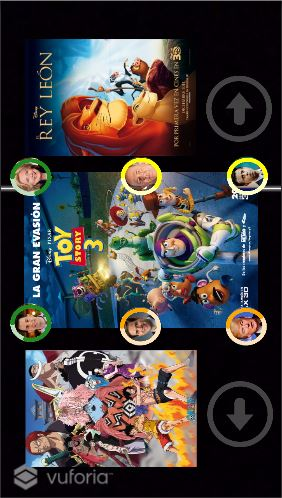
\includegraphics[width=3in, angle=270]{figures/chapter-2/recomendadorAR.JPG}
        \caption{Vista encargada de recomendar planes en RA al enfocar a un amigo}
    \end{figure}
    
\end{flushleft}
\newpage
\section{Fuentes de información}
\label{makereference2.3}
Como nuestra aplicación muestra información sobre las películas que se recomiendan y que los usuarios han guardado, hemos
tenido que investigar de que página web podríamos obtener estos datos tan relevantes.
\paragraph{IMDB:}
Nos decidimos por usar la página web de \textbf{IMDB}: \url{https://www.imdb.com/} para conseguir las valoraciones, resúmenes, nombre del director,
género y país de las películas, entre otros datos, debido a que consideramos que es de las webs más usadas entre los cinéfilos y posibles 
usuarios de nuestra aplicación.

\section{Técnicas de recomendación}
\label{makereference2.4}
En nuestra aplicación, tenemos los siguientes datos para nuestro sistema de recomendación: \textbf{Información de usuarios}, \textbf{Información de películas} y \textbf{Valoraciones de los usuarios a las películas}.
Entre los distintos tipos de sistemas de recomendación, vamos a destacar dos, pues son los que mejores asemejan a nuestra situación.

\begin{itemize}
    \item \textbf{Filtrado Colaborativo:} A este sistema de recomendación se basa en buscar usuarios que tienen preferencias similares. Entonces si a un individuo le ha gustado una película, entonces se le recomiendan las películas que les gustaron a otros pero que también les gustaron esta.
    \item \textbf{Filtrado basado en el contenido:} Esta basado como lo indica su nombre, en su contenido, si a alguien le gusta una película, se le va a recomendar otra que es parecida.
\end{itemize} 

\begin{figure}[H]
    \centering
    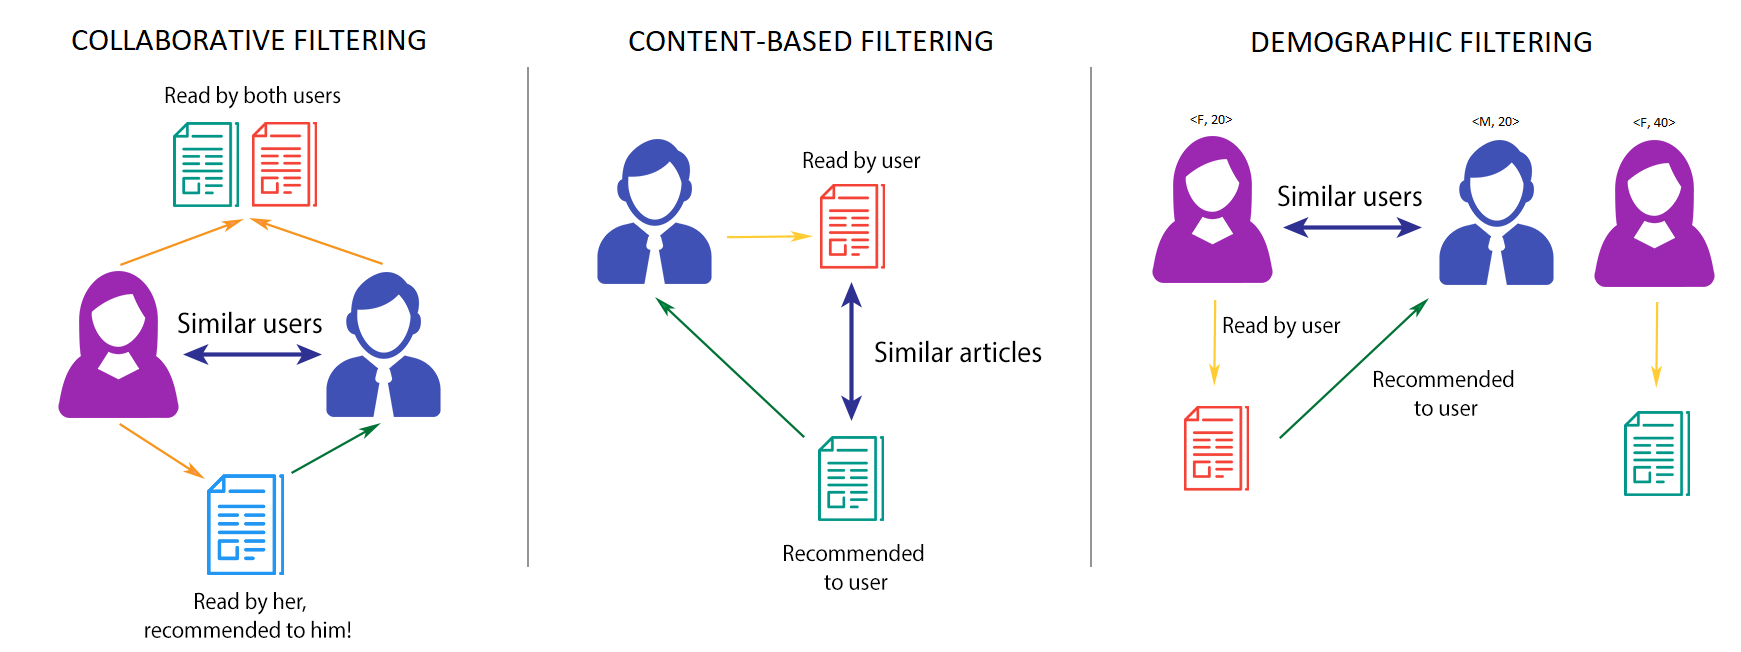
\includegraphics[width=3in, angle=0]{figures/chapter-2/recommendation_systems.png}
    \caption{Tipos de sistemas de recomendación}
\end{figure}

Decidimos para la aplicación el sistema de \textbf{Filtrado Colaborativo} por los siguientes motivos:

\begin{itemize}
    \item Tenemos valoraciones de usuarios a películas que podemos aprovechar, ya que es una de las acciones que puede realizar un usuario y se aprovecha para recolectar los datos.
    \item Hemos conseguido un archivo csv de unos 200000 valoraciones de usuarios a películas con sus respectivos títulos. El cual solo tendríamos que crear los usuarios ficticios para conseguir una base inicial de datos para la base de datos.
    \item Para usar el filtrado basado en el contenido tenemos que diseñar muy bien los datos de cada uno de las entidades, además de aplicar los pesos de importancia a los atributos para en un futuro aplicar el sistema.  
\end{itemize} 


% +--------------------------------------------------------------------+
% | Sample Chapter 3
% +--------------------------------------------------------------------+

\cleardoublepage

% +--------------------------------------------------------------------+
% | Replace "This is Chapter 3" below with the title of your chapter.
% | LaTeX will automatically number the chapters.
% +--------------------------------------------------------------------+

\chapter{Diseño de la aplicación}
\label{makereference3}



\section{Escenarios}
\label{makereference3.2}
Antes de decidir como implementaríamos nuestra aplicación decidimos que sería importante establecer una serie
de escenarios en los que podría ser usada. Tras esto pudimos ponernos de acuerdo en qué funcionalidades incluiríamos y que 
éstas se ajustasen a las necesidades de los usuarios. Además, estos escenarios deberían usar la Realidad Aumentada para que 
les aporte valor, ya que, como hemos expuesto anteriormente en el capítulo 2, el grueso de nuestra aplicación se centra en esta tecnología.

\paragraph{Escenario 1. Usando la aplicación en casa:\\}
\begin{itemize}
    \item Te apetece ir al cine y encuentras el cartel de una película que te interesa ver en cualquier lado (ordenador, revista, etc.), sacas tu móvil con la aplicación y 
    la escaneas, con la realidad aumentada te saldrán los distintos paneles y botones que te facilitan información sobre la película:
    \begin{enumerate}
        \item Ver el tráiler.
        \item Valoración que tiene en páginas web, como por ejemplo \textbf{IMDB}.
        \item Botón para crear un plan para ir a ver esa película o unirte a uno que uno de tus amigos ya haya creado para esa misma película.
        \item Botón para guardar la película en tu lista de películas guardadas.
    \end{enumerate}
    \item Te apetece ir al cine y has visto varias películas que te interesan, pero no sabes a cuál ir, captas todas ellas con la aplicación 
    y para cada una de ellas tendrás las opciones anteriores más poder crear un nuevo plan o guardarlas para ver su información más tarde.
\end{itemize}
\newpage
\paragraph{Escenario 2. Usando la aplicación en la calle.\\}
\begin{itemize}
\item En este escenario, queremos solucionar el problema que aparece cuando el usuario de la aplicación se encuentra con el cartel de una película y pretende registrarla en su aplicación lo más rápido posible.
Este escenario se produce mayormente cuando el usuario está paseando por la calle, en el metro, en un centro comercial, etc.
\\
El usuario podrá rápidamente escanear el cartel de la película y guardar así ésta en su lista de películas para posteriormente añadirla a un plan o poder ver la información de ésta, además de la opción de poder valorarla.
\\
Este escenario requiere que el usuario guarde rápidamente la película, puesto que el usuario puede tener prisa y simplemente esté pasando cerca de un cartel mientras va a otro sitio.
\end{itemize}



\section{Requisitos funcionales}
\label{makereference3.3}

\paragraph{\large Planes:\\}

Los planes están compuestos por una película, un usuario creador del plan, y los usuarios que se hayan unido. El plan
es creado debido a la necesidad que tiene un usuario de querer ver una película específica, con una serie de usuarios que 
entrarán en el plan por tener interés en ver la misma película debido a su afinidad con ella.
\\
\textbf{Funciones:}
\begin{enumerate}
    \item \textbf{Crear plan}: para crear un plan, un usuario ha tenido que guardar previamente una película tras reconocerla con la cámara y al entrar a la interfaz de la información de la película podrá presionar el botón para crear un plan con dicha película.
    \item \textbf{Unirse a un plan}: solo podrán unirse los amigos del usuario creador del plan, al entrar en la interfaz que tiene la información de un plan podremos pulsar un botón para unirnos.
    \item \textbf{Información de un plan}: simplemente con presionar en un plan podremos ver la información del mismo, es decir, la película a ver y los usuarios que se han unido.
\end{enumerate}
\newpage
\paragraph{\large Películas guardadas:\\}

Las películas guardadas son aquellas que el usuario ha decidido guardar para ver su información más tarde o para posteriormente añadirlas a un plan.
\\
\textbf{Funciones:}
\begin{enumerate}
    \item \textbf{Guardar película}: cuando un usuario reconoce una película con la cámara, le aparecerá un botón que le permitirá guardar la película como favorita, para poder ver su información posteriormente o crear un plan con ella. También podrá guardar la película si la encuentra mediante la barra de búsqueda pulsando un botón con el mismo icono.
    \item \textbf{Información de una película}: un usuario puede ver la información de una película que haya guardado con presionar en la misma. Podrá ver una pequeña sinopsis, el género y el director, además de la posibilidad de poder valorarla o acceder a su traíler en Youtube.
\end{enumerate} 

\section{Sistema de recomendación}
\label{makereference3.5}
Para la implementación de los sistemas de recomendación hemos encontrados tres librerías:
\begin{enumerate}
    \item \textbf{Mahout}: Se trata de una librería bastante compleja, que básicamente abarca la mayoría de necesidades para la implementación del sistema de recomendación.
    \item \textbf{Lenskit}: Es otra librería de \textbf{Java} para la implementación de sistemas de recomendación.
    \item \textbf{LibRec}: Se trata de una librería de terceros que está subida en un repositorio de \textbf{GitHub}.
\end{enumerate}

Al final nos hemos decantado por \textbf{Mahout}, ya que aporta una documentación más completa. Otro de los motivos es que ofrece clases para realizar la conexión directamente con la base de datos 
sin tener que leer desde ficheros csv. Por otro lado, en el testeo de 
\textbf{Lenskit}, cuando intentábamos reproducir el ejemplo que ofrecían, nos encontramos que algunas funciones estaban 
obsoletas y, por tanto, no nos transmitía mucha confianza. Por último, \textbf{Mahout} destaca por ser más fácil de usar y minimizar nuestro esfuerzo en aprender esta nueva tecnología.

\section{Prototipos}
\label{makereference3.6}

\subsection{ARCore} 
\label{makereference3.6.1} 
\begin{flushleft}
    Al comenzar la fase de desarrollo de proyectos, pensamos que una de las tecnologías que debíamos 
    investigar y probar debía ser \textbf{ARCore}. Esto se debía a que, la empresa detrás de esta 
    tecnología es \textbf{Google} y esto podría significar que tendríamos más material de consulta 
    y ejemplos en comparación con otras tecnologías de fabricantes con menos recursos.
    \textbf{ARCore} se encuentra disponible para \textbf{Java}, \textbf{Unity}, \textbf{Unreal} e \textbf{iOS}. Comenzamos realizando el 
    "Quickstart" para \textbf{Android} y posteriormente para \textbf{Unity}. 
    Tras realizar los proyectos propuestos por \textbf{ARCore}, realizamos algún proyecto propio 
    para comprobar si la herramienta se ajustaba a la idea que teníamos para nuestro futuro proyecto.
    Tras realizar ambos proyectos, concluimos que, aunque \textbf{ARCore} reúne las características 
    necesarias para en un futuro convertirse en una de las tecnologías más importantes en Realidad Aumentada, 
    no íbamos a seleccionarla para nuestro proyecto por las siguientes razones:
    \begin{enumerate}
        \item \textbf{ARCore} dispone de mucha documentación para comenzar a usar la herramienta, pero poca para realizar tareas más complejas
        \item \textbf{ARCore} resulta muy útil para realizar superposiciones de modelos 3D sobre superficies, sin embargo, una de las funcionalidades más importantes que nuestra aplicación requería era la interacción con la realidad aumentada mediante el uso de botones, imágenes y la carga dinámica de elementos para posicionar en la pantalla de Realidad Aumentada e interaccionar con el usuario. En este sentido \textbf{ARCore} no está, por el momento, tan preparada como otras tecnologías.
    \end{enumerate}
    
\end{flushleft}
\subsection{Viro Media} 
\label{makereference3.6.2}
\begin{flushleft}
El objetivo del prototipo realizado con \textbf{Viro Media} es reconocer imágenes almacenadas en el dispositivo para mostrar texto y
 objetos virtuales. Además de probar tecnologías de desarrollo móvil web como en este caso \textbf{React Native}
 para plataformas \textbf{iOS} y \textbf{Android}.
\end{flushleft}
\begin{flushleft}
Comenzamos construyendo una interfaz sencilla con botones que nos redirigen a la escena de Realidad Aumentada.
Para esta interfaz utilizamos \textbf{NativeBase} que es una librería que nos permite
realizar una aplicación con apariencias de tipo \textbf{iOS} o \textbf{Android} según el dispositivo.
\end{flushleft}

\begin{figure}[htb]
    \centering
    \makebox[0pt][c]{%
    \begin{minipage}[b]{0.5\linewidth}
    \centering
      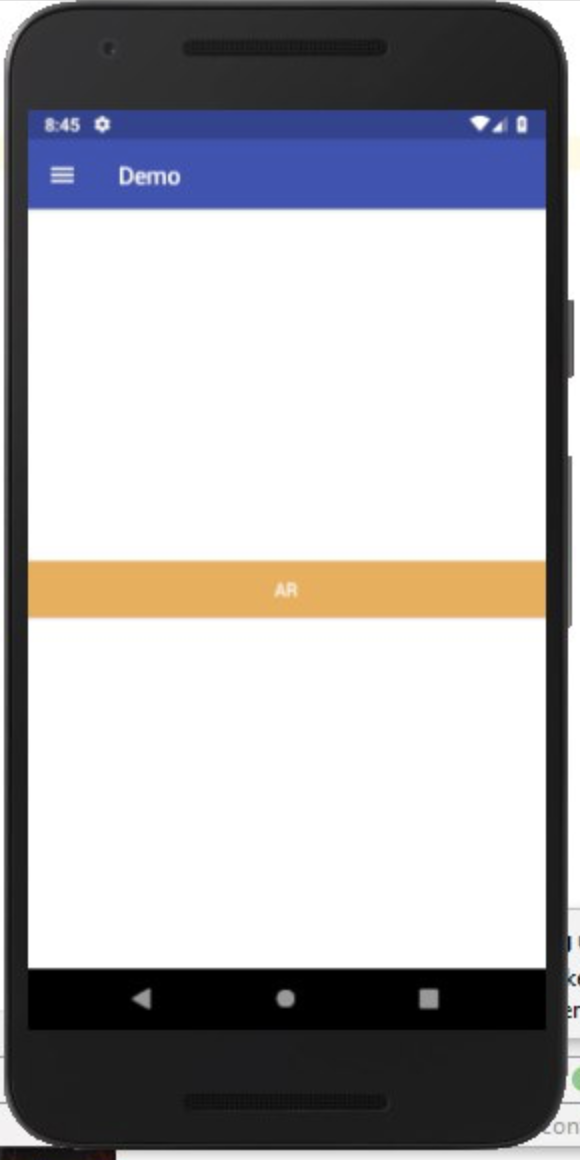
\includegraphics[scale=0.3]{figures/chapter-3/viromedia/android.png}
      \caption{Visualización con NativeBase en Android}
    \label{sva}
    \end{minipage}%
    \hspace{0.3cm}
    \begin{minipage}[b]{0.5\linewidth}
    \centering
     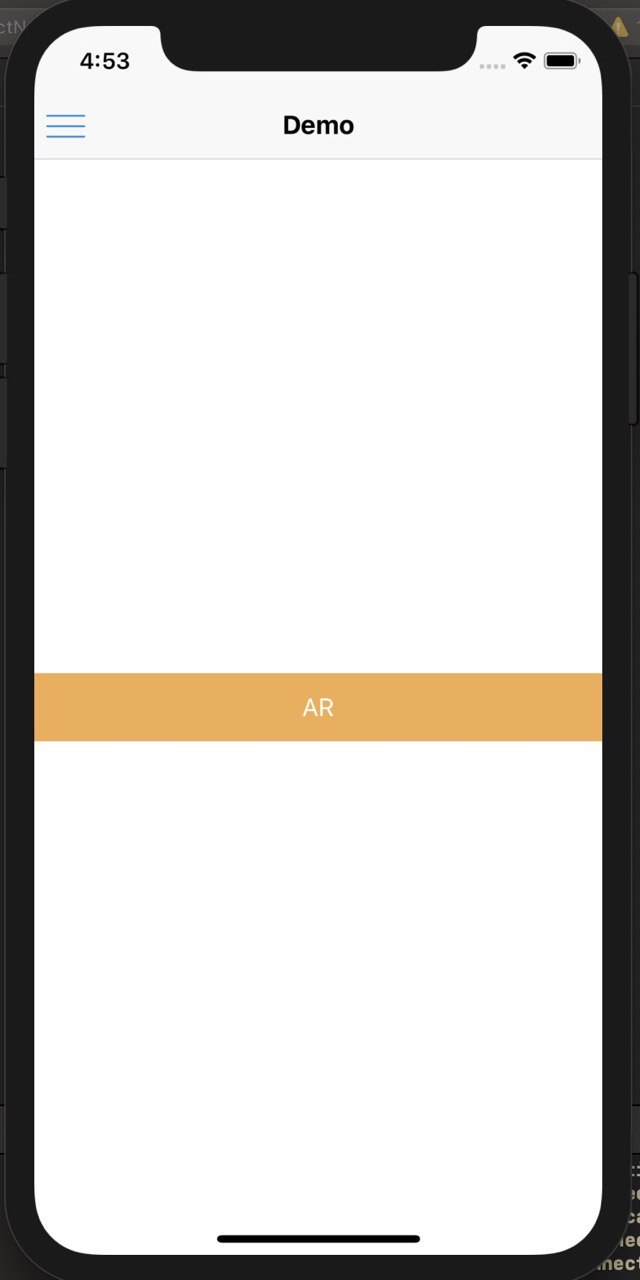
\includegraphics[scale=0.3]{figures/chapter-3/viromedia/ios.jpg}
      \caption{Visualización con NativeBase en iOS}
    \label{svb}
    \end{minipage}%
    }%
\end{figure}

\begin{flushleft}
Para la escena de Realidad Aumentada mostramos texto y al detectar el póster de Pantera Negra,
 reacciona mostrando una animación de dicho súper héroe saliendo del póster.
\end{flushleft}
 
\begin{figure}[H]
    \centering
    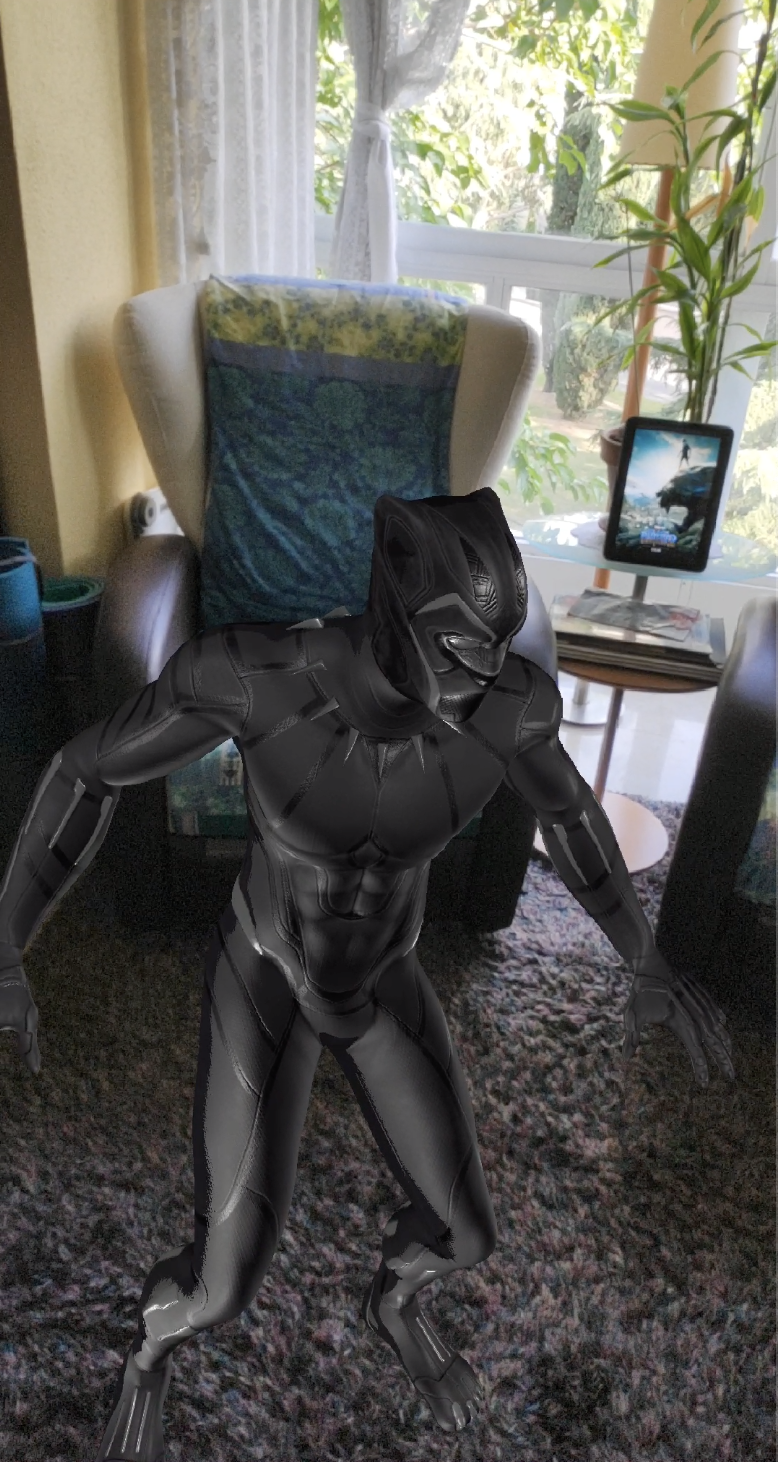
\includegraphics[width=3in]{figures/chapter-3/viromedia/blackpanther.png}
    \caption{Visualización de RA}
\end{figure}

\begin{flushleft}
Una de las ventajas que apreciamos fue la facilidad del lenguaje, en este caso \textbf{Javascript},
 utilizando la popular librería \textbf{ReactJS} y la buena documentación de \textbf{Viro Media}
 que hacían que el proceso de codificación fuera agradable.
\end{flushleft}
\begin{flushleft}
Uno de los problemas que presentaba este prototipo era que las dependencias de \textbf{Viro Media} entraban en conflicto con las de \textbf{NativeBase}
imposibilitándonos la forma de encontrar versiones compatibles. Utilizamos las últimas que, a pesar de lanzar
 advertencias, funcionaba en el ejemplo realizado.
Otro problema fue la compilación de la aplicación, \textbf{Viro Media} tiene una aplicación para probar lo
 que desarrollamos conectándose a nuestro ordenador a través de la red. El problema es
 que algunos recursos, como los iconos que utilizaba \textbf{NativeBase}, no eran descargados, por lo que la
 mejor forma era probar la versión compilada de \textbf{iOS} y \textbf{Android}. La forma de compilar
 la aplicación era un proceso costoso para los ordenadores, lento y con multitud de problemas según
 se ampliaban las librerías que se utilizan.
\end{flushleft}

\begin{flushleft}
La conclusión que obtuvimos de este prototipo fue que \textbf{Viro Media} y \textbf{React Native} son tecnologías muy prometedoras, pero debido a los
 problemas surgidos y a que todas sus versiones no eran estables vimos un claro riesgo para
 nuestro proyecto.
\end{flushleft}

\newpage
\subsection{Vuforia + Android} 
\label{makereference3.6.3} 
 
\begin{flushleft}
En este prototipo utilizamos la librería nativa de \textbf{Vuforia} para \textbf{Android} para 
realizar las pruebas de tecnología de reconocimiento de imágenes tanto en  
local como usando la nube que nos ofrecía \textbf{Vuforia}, para la posterior renderización
de objetos y textos.

Las características tecnológicas de este prototipo son las siguientes:
\end{flushleft}

\begin{enumerate}
    \item La librería de \textbf{Vuforia} para \textbf{Android} está diseñada a muy bajo nivel.
    \item \textbf{Vuforia} para dibujar en 3D usa la librería \textbf{OpenGL}.
    \item \textbf{OpenGL} utiliza una serie de espacios donde se van colocando los elementos: 
    \begin{enumerate}
        \item \textbf{Local space}: Es el espacio local de cada objeto.
        \item \textbf{World space}: Es el mundo donde se encuentran los objetos.
        \item \textbf{View space}: El mundo visto desde la perspectiva de la cámara.
        \item \textbf{Clip space}: Se integra con la pantalla del móvil y, definiendo los límites visibles, se establecen unas coordenadas de rango (-1,-1) - (1,1).
    \end{enumerate}
    \begin{flushleft}
        Las transformaciones de estos espacios se realizan mediante matrices 4x4, 
        en las que la primera fila hace referencia a la coordenada x, la segunda a la coordenada y y la 
        tercera a la coordenada z, mientras que la última columna hace referencia a los desplazamientos 
        de los objetos en esos 3 ejes.
        \end{flushleft}
        

        
            \begin{figure}[H]
                \centering
                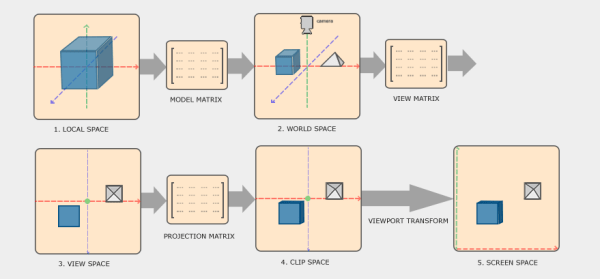
\includegraphics[width=5in]{figures/space-transformation.png}
                \caption{Esquema de los distintos espacios que usa OpenGL}
            \end{figure}

            \begin{figure}[H]
                \centering
                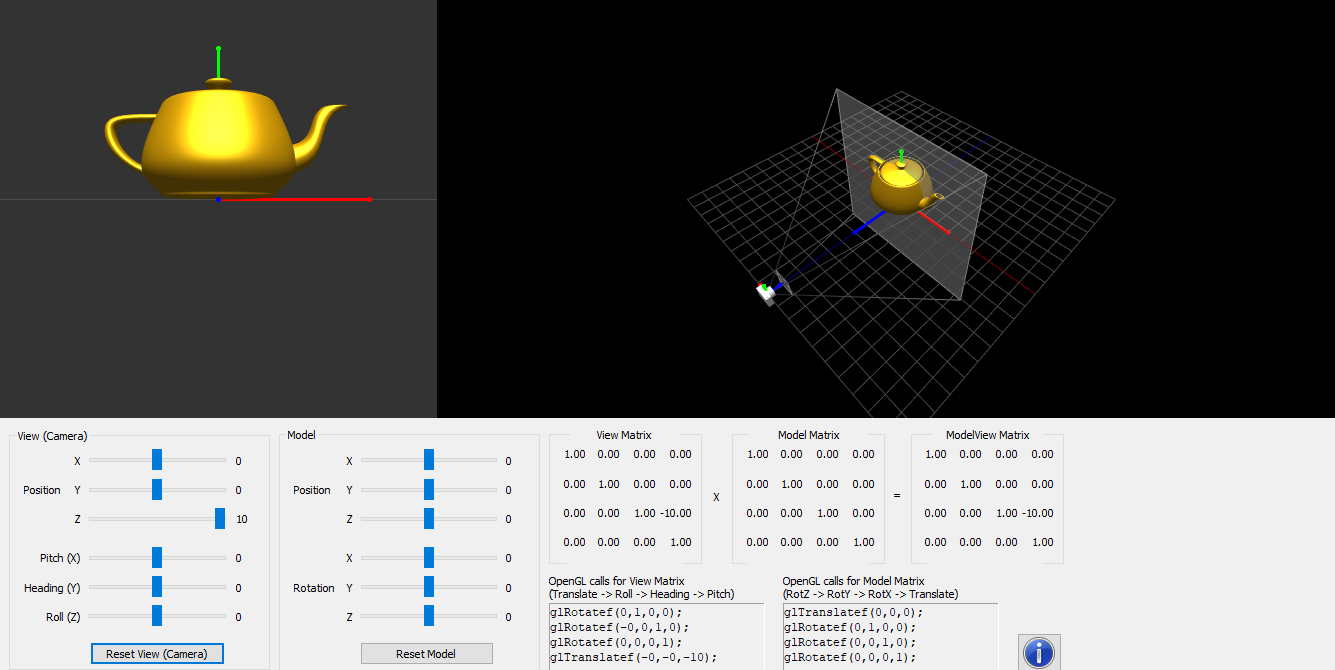
\includegraphics[width=5in]{figures/teapot.png}
                \caption{Ejemplo de un modelo en 3D}
            \end{figure}
    
    \item En \textbf{OpenGL} es necesario escribir código para que las tarjetas gráficas rendericen el modelo 3D,
    el lenguaje que se usa es \textbf{GLSL}. Este código de \textbf{GLSL} se escribe en forma de \textbf{String} y se llama a un método 
    que proporciona \textbf{OpenGL}.
    \begin{figure}[H]
        \centering
        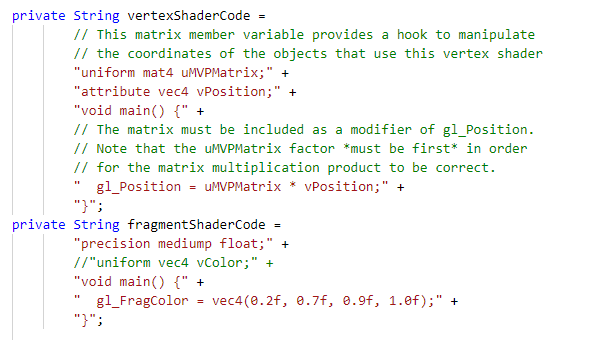
\includegraphics[width=5in]{figures/GLSL.png}
        \caption{Código en GLSL}
    \end{figure}
        
    \item Otro aspecto a tener en cuenta es que \textbf{OpenGL} solo nos ofrece lo básico, no nos ofrece métodos para dibujar 
    directamente objetos, sino que hay que seguir un pipeline de procesos para conseguir dibujar algo.
    \newline
    \begin{flushleft}
    Esto consiste en pasar un \textbf{array} de números (cada tres para definir un punto) 
    a las tarjetas gráficas, establecer triángulos entre los puntos (más arrays de números) 
    definir colores a partir de los puntos (más arrays)..., y con el código del shader, ejecutar 
    estos datos.
    \begin{figure}
        \centering
        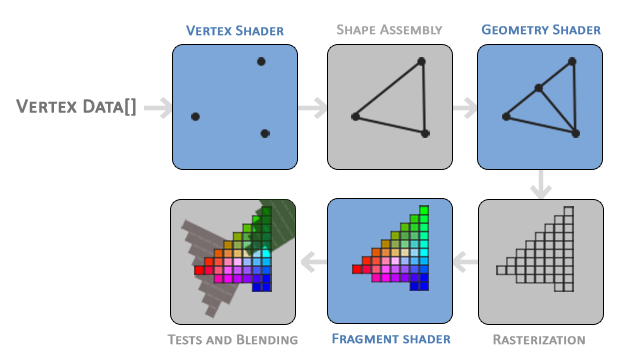
\includegraphics[width=4in]{figures/pipeline.png}
        \caption{Pipeline de la construcción de un modelo}
    \end{figure}
    \end{flushleft}
    \newpage
    \item Por último, como sólo ofrece métodos básicos, no hay métodos de escritura de texto, y la forma que 
    encontramos y que funcione fue usar un bitmap con los caracteres. Rechazamos esto por un principal motivo, para hacer que funciones hay que codificar a muy bajo nivel y 
    nos costaría mucho tiempo y esfuerzo.
    \begin{figure}
        \centering
        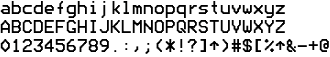
\includegraphics[width=5in]{figures/bitmap-font.png}
        \caption{Mapa de bits de caracteres usado}
    \end{figure}
\end{enumerate}
 

\newpage
\subsection{Vuforia + Unity} 
\label{makereference3.6.4}
\begin{flushleft}
    Para realizar este prototipo utilizamos \textbf{Unity} como herramienta básica para realizar la aplicación y \textbf{Vuforia} para dar soporte a la Realidad Aumentada.
    El prototipo a desarrollar consistió en un modelo 3D de un dragón que aparecía al detectar una imagen que previamente habíamos establecido como ``imagen objetivo''.
\end{flushleft}
    \begin{figure}[H]
        \centering
        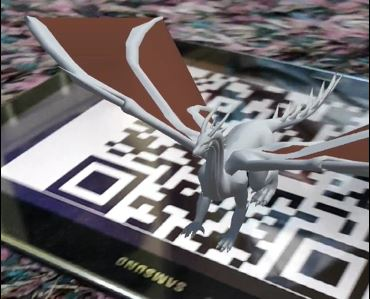
\includegraphics[width=5in]{figures/prototipoUnity.jpg}
        \caption{Modelo en 3D que aparecía al detectar la imagen}
    \end{figure}
\begin{flushleft}
    Pese a que nadie del equipo había utilizado \textbf{Unity} previamente el resultado fue bastante positivo ya que:
    \begin{enumerate}
    \item \textbf{Unity} resultó ser intuitivo y relativamente fácil en cuanto al aprendizaje de las funcionalidades básicas.
    \item \textbf{Vuforia} parecía estar muy probada e incluía de serie muchas funcionalidades.
    \item \textbf{Vuforia} tenía la opción de utilizar un \textbf{Cloud} para almacenar las imágenes objetivo.
    \end{enumerate}
\end{flushleft}

\subsection{Vuforia + Unity + Android} 
\label{makereference3.6.5}
\begin{flushleft}
Una vez realizado el prototipo en \textbf{Vuforia} con \textbf{Unity} comenzamos a investigar cómo realizar el resto de la aplicación que no requería de Realidad Aumentada.
\break
Hasta este momento teníamos claro que \textbf{Vuforia} con \textbf{Unity} era la mejor combinación para realizar la parte de Realidad Aumentada, sin embargo, \textbf{Unity} no era igual de intuitivo ni eficaz a la hora de realizar tareas propias de una aplicación "normal", como el desarrollo de interfaces o la lógica.
\break
Por este motivo intentamos buscar la opción de realizar una aplicación en la que la Realidad Aumentada estuviese diseñada en \textbf{Unity} con \textbf{Vuforia} y el resto de la aplicación en Android.
\end{flushleft}
\begin{figure}[H]
        \centering
        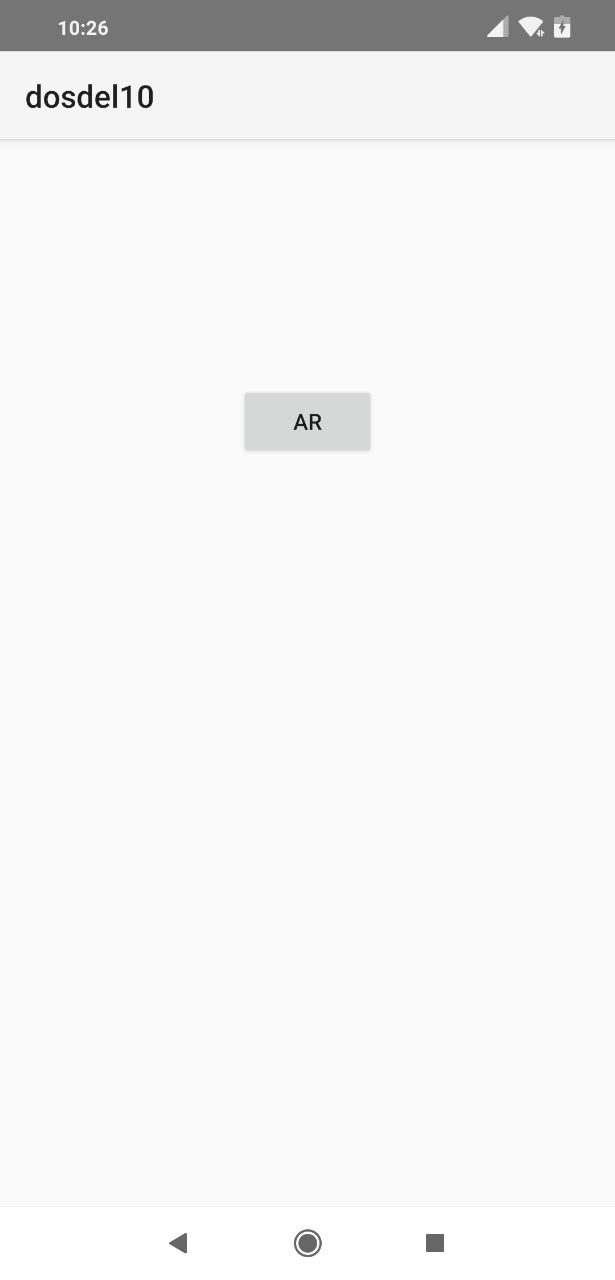
\includegraphics[width=1in]{figures/androidUnityVuforia.jpg}
        \caption{Botón que comunicaba Android con Unity}
\end{figure}
\begin{flushleft}
    Finalmente conseguimos tener ambos proyectos independientes, la Realidad Aumentada se desarrollaba en \textbf{Unity} con \textbf{Vuforia} y se exportaba a un proyecto Android donde se encontraba el resto de la aplicación.
    Esto nos permitía realizar la Realidad Aumentada con la herramienta que tras las primeras tomas de contacto habíamos comprobado que era la mejor (\textbf{Unity} con \textbf{Vuforia}) y del mismo modo realizar el resto de la aplicación con la mejor herramienta para esta parte (AndroidStudio).
\end{flushleft}
\begin{flushleft}
    Tras realizar este prototipo, consideramos que estas herramientas podrían ser las que usásemos en la aplicación final puesto que:
    \begin{enumerate}
    \item Como ya habíamos descubierto en el prototipo anterior, \textbf{Unity} era una herramienta muy completa y junto con \textbf{Vuforia} nos proporcionaban todas las herramientas necesarias para cumplir con los casos de uso de Realidad Aumentada que teníamos en mente.
    \item Al haber encontrado la forma de combinar \textbf{Unity + Android} no teníamos que renunciar a ninguna de las dos herramientas. Lo que nos permitía explotar las cosas buenas de ambas herramientas.
    \item La comunicación entre \textbf{Unity} y Android era relativamente sencilla pese a ser dos proyectos distintos.
    \end{enumerate}
\end{flushleft}

\newpage
\subsection{Server en Spring} 
\label{makereference3.6.6}

\begin{flushleft}
    Para la realización de la parte backend de la aplicación decidimos
    incorporar la tecnología de \textbf{Spring} para codificar un \textbf{servicio web REST} en \textbf{Java}
    y el acceso a datos mediante \textbf{MySQL}.
\break
\break
    Para el prototipo seguimos el siguiente tutorial: 
\newline
Cómo crear un microservicio o servicio web REST con Spring Boot\cite{tutorialspring}
\break
    que consistía en 3 partes bien definidas para la creación de dicho \textbf{servicio web REST} para la gestión de una entidad de contactos muy simple, se puede observar su estructura
    en la figura 3.6.
    \begin{figure}[H]
        \centering
        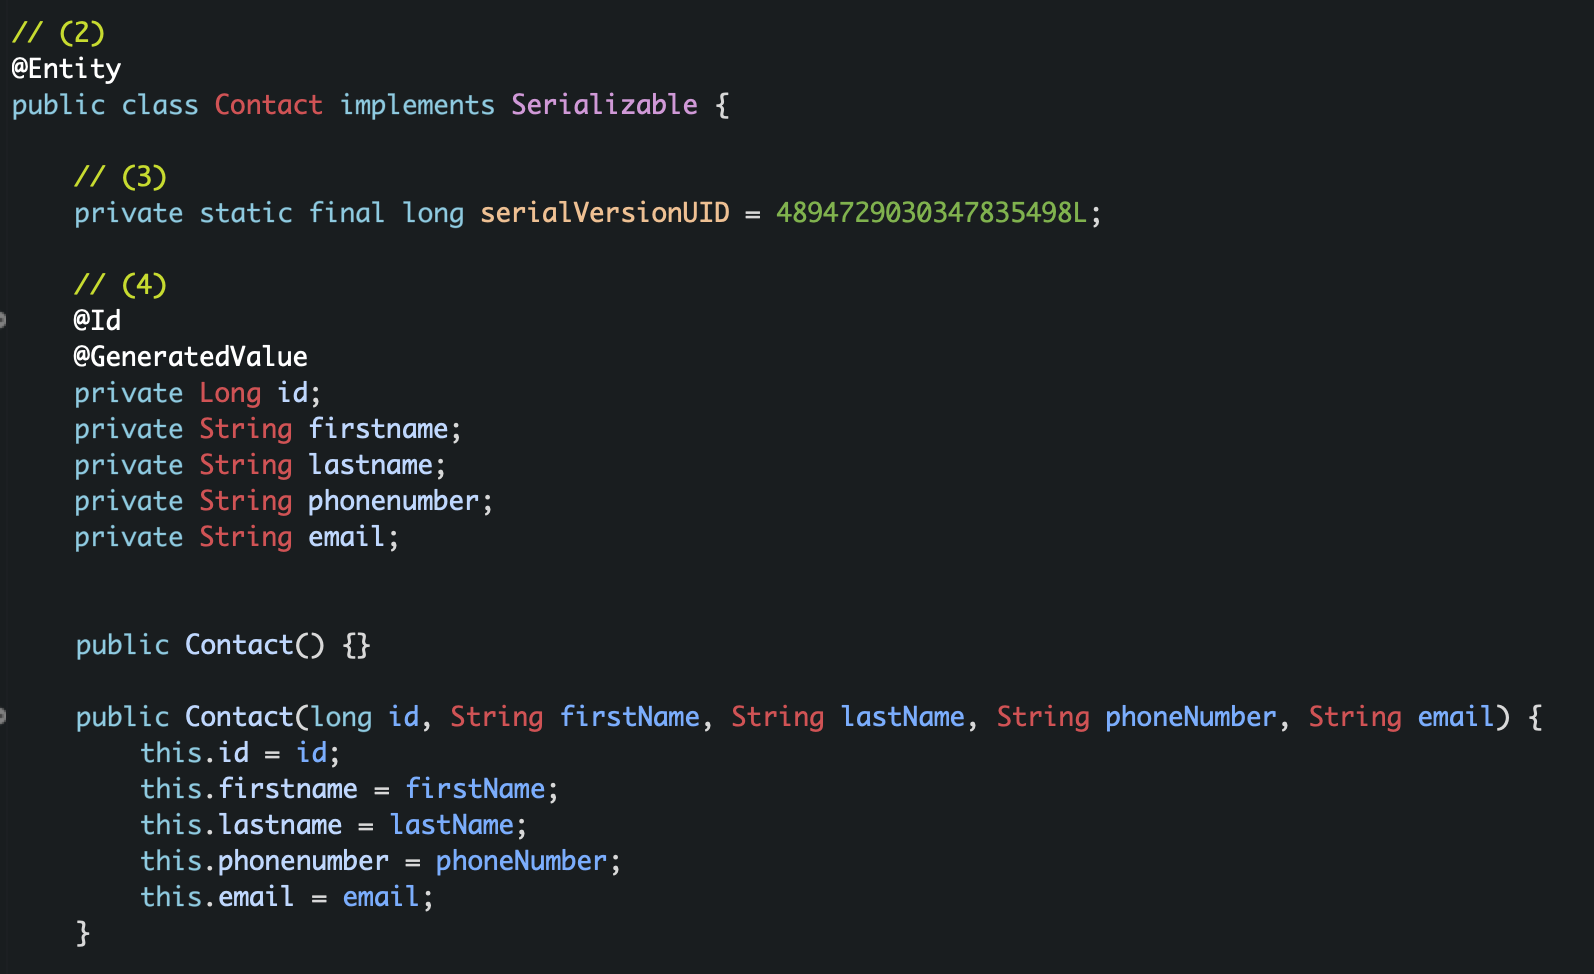
\includegraphics[width=6in]{figures/ContactsEntity.png}
        \caption{Entidad de Contactos}
    \end{figure}
\break
\break
    También se investigaron distintas formas de realizar el acceso a la base de datos desde el servidor, pero finalmente nos decantamos por usar la
    clase \textbf{JPARepository} o \textbf{CRUDRepository}, las cuales nos ofrecen ya implementados los métodos típicos de las operaciones \textbf{CRUD}, además de la opción 
    de poder crear nuestros propios métodos.
\end{flushleft}

\begin{flushleft}
    Para poder probar las distintas peticiones de tipo \textbf{POST} y \textbf{GET}, que realizamos en local, usamos la herramienta 
    \textbf{Postman}, ver figura 3.7.
    \begin{figure}[H]
        \centering
        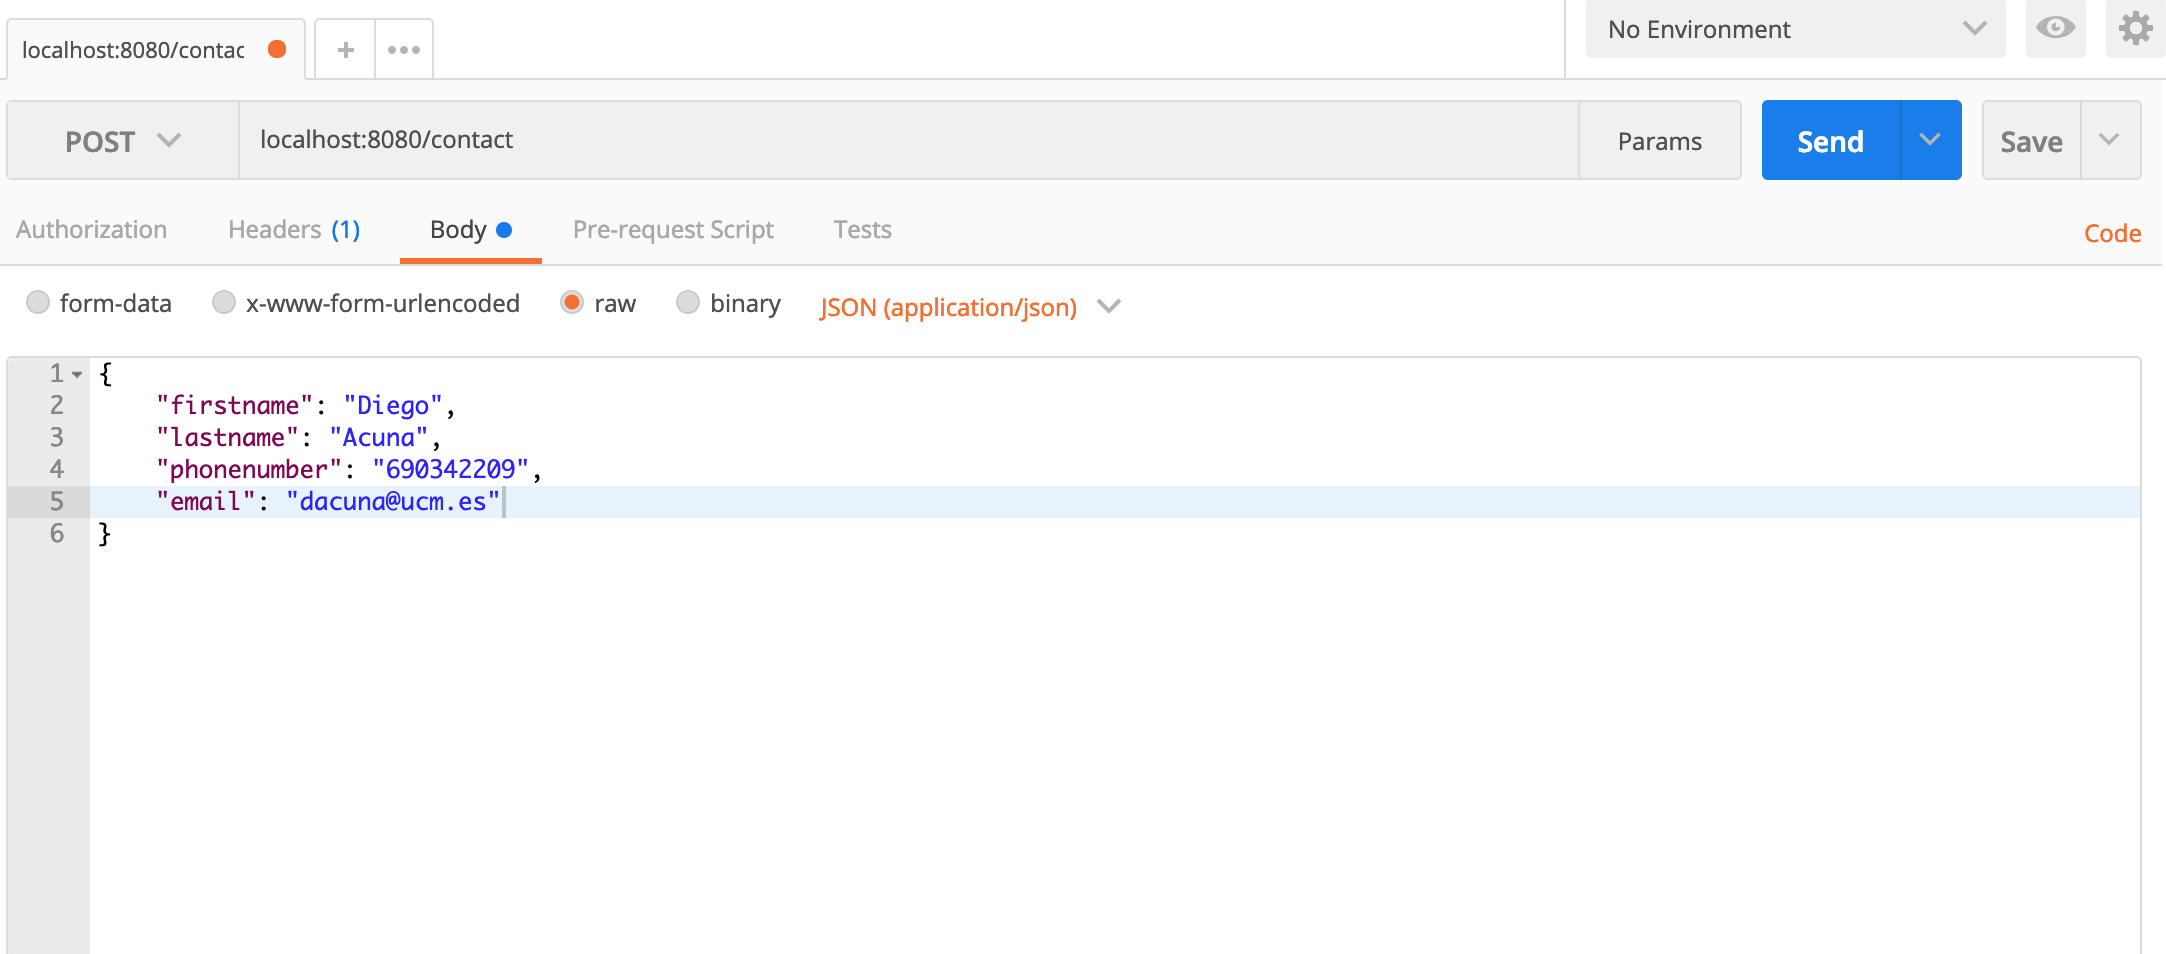
\includegraphics[width=6in]{figures/Postman.png}
        \caption{Postman}
    \end{figure}
    Para este prototipo decidimos usar \textbf{MySQL} como sistema de gestión de bases de datos relacional, aunque
    a la hora de probar a levantar nuestro servidor de prueba tuvimos que rehacer este prototipo, además de adaptarlo para 
    que gestionara entidades de películas, y que usara \textbf{PostgreSQL}, además de cambiar una serie de anotaciones y limpiar 
    el archivo \textbf{pom.xml} de líneas de código innecesarias, ver figura 3.8, que es el que contiene las dependencias de nuestro proyecto.
    \begin{figure}[H]
        \centering
        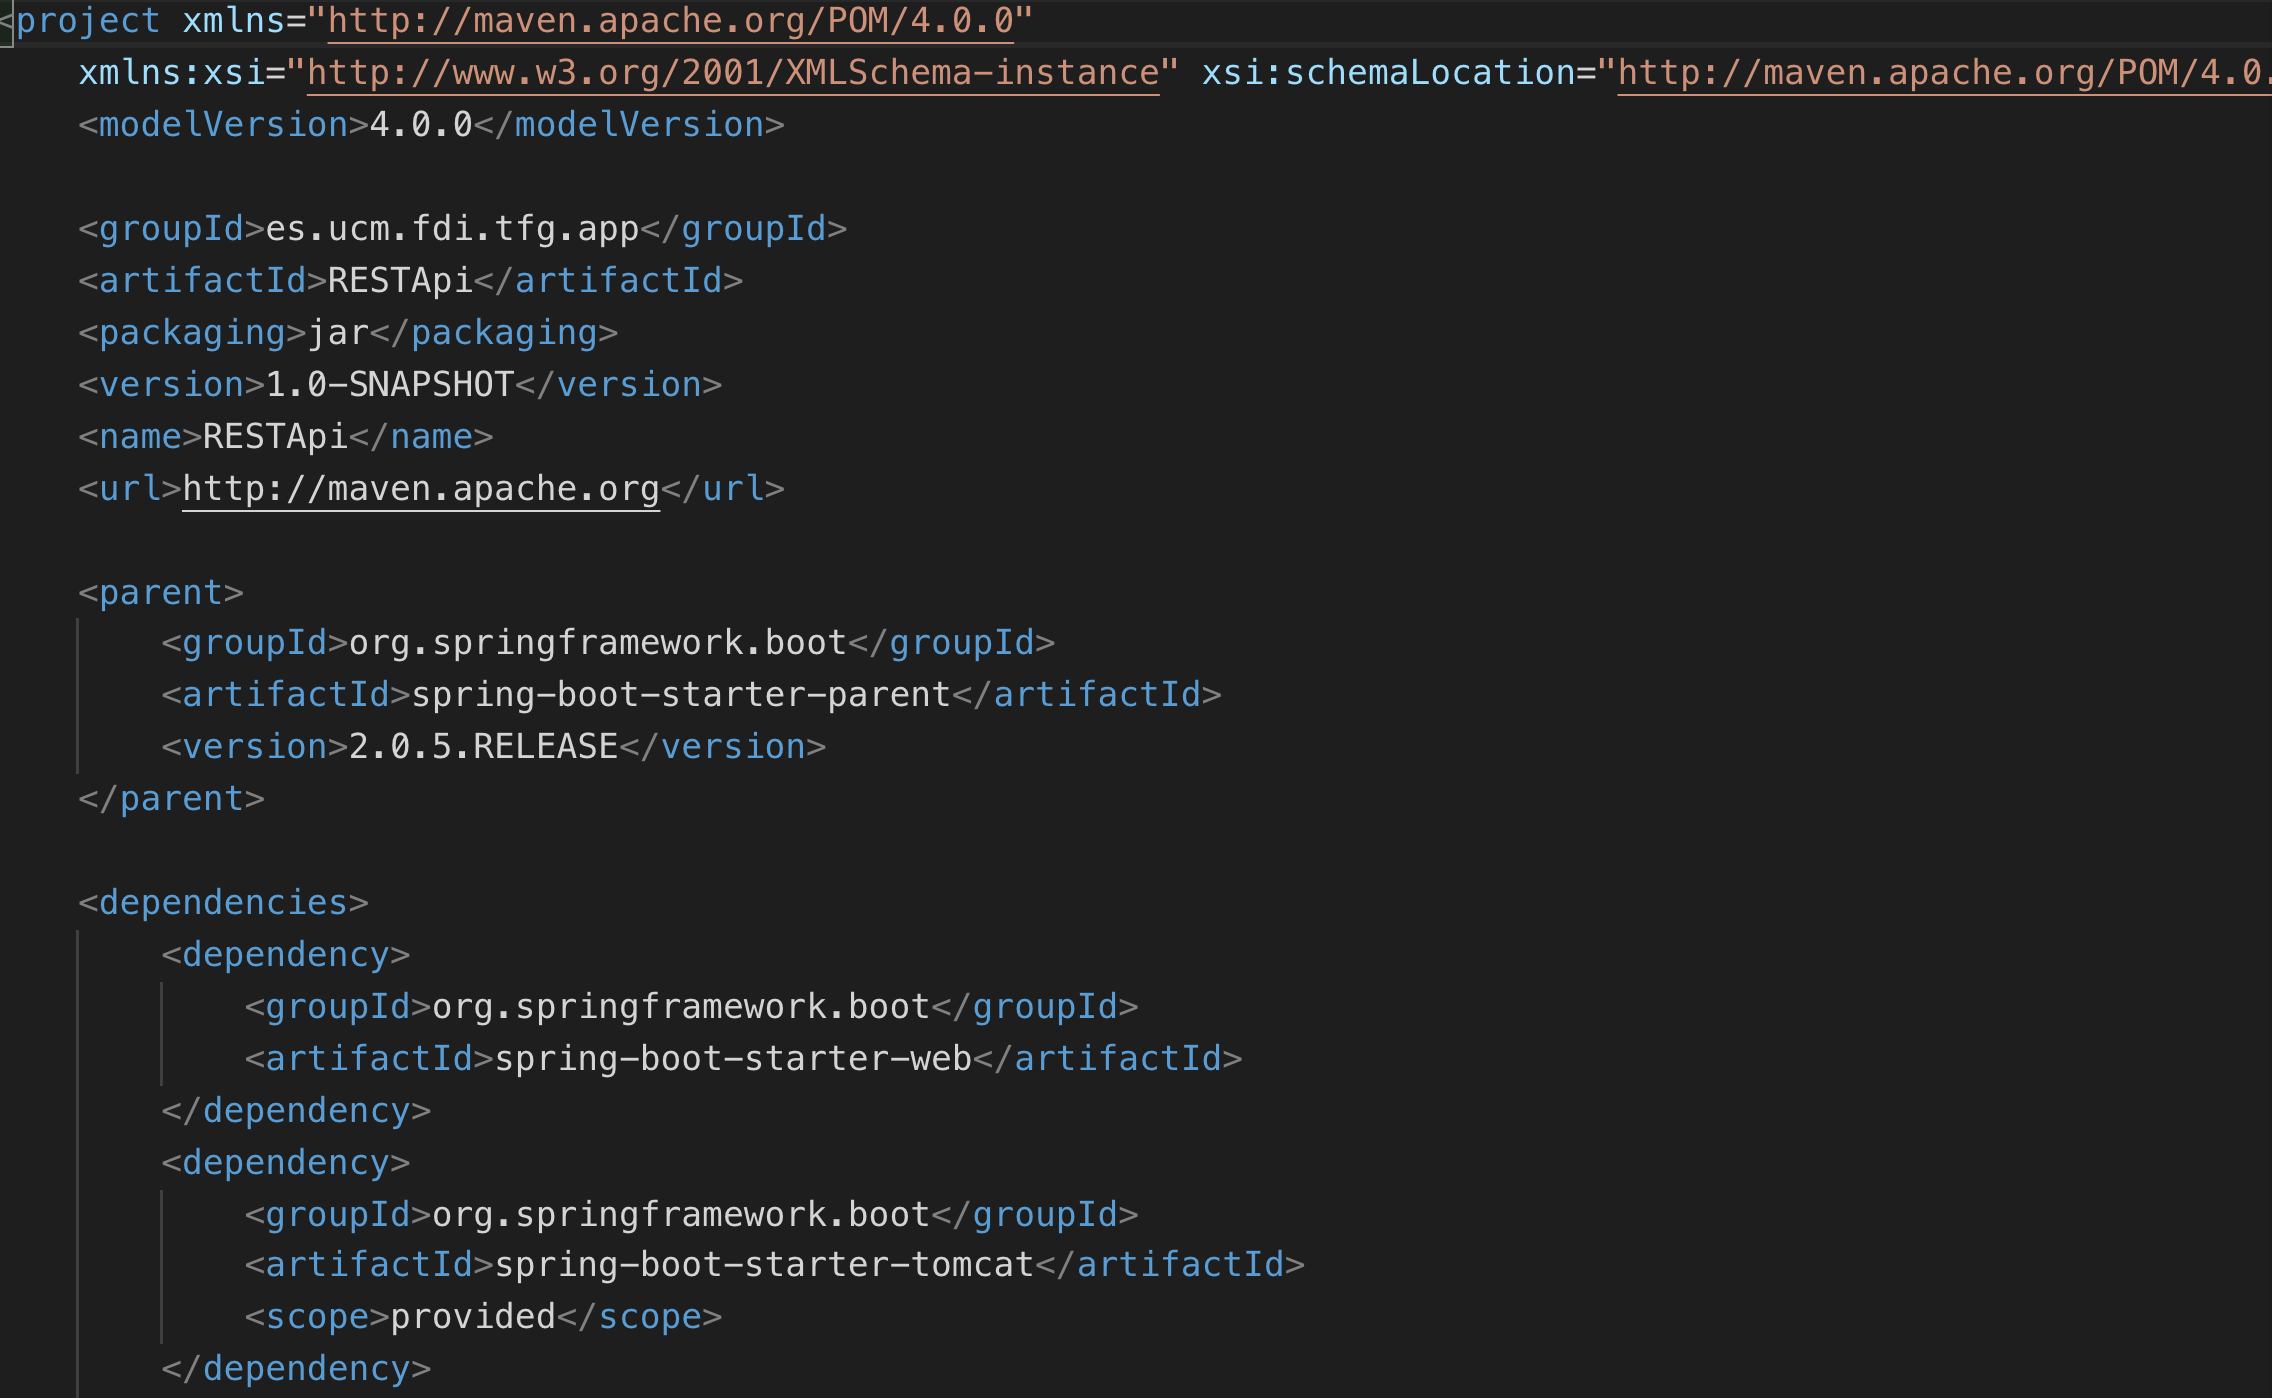
\includegraphics[width=6in]{figures/PomXML.png}
        \caption{Archivo pom.xml}
    \end{figure}
\end{flushleft}
\section{Interfaz de usuario}
\label{makereference3.4}

A continuación, mostraremos las distintas interfaces de usuario de nuestra aplicación y la evolución que han ido sufriendo.
\subsection{Interfaz de lista de planes}
\label{makereference3.4.1}
El objetivo de esta vista es el de mostrar los planes públicos que existen, indicando con una imagen de fondo la película para la que se creó el plan, el usuario
que creó dicho plan y los usuarios que se han unido. La primera vista que realizamos fue la siguiente
\begin{figure}[H]
    \centering
    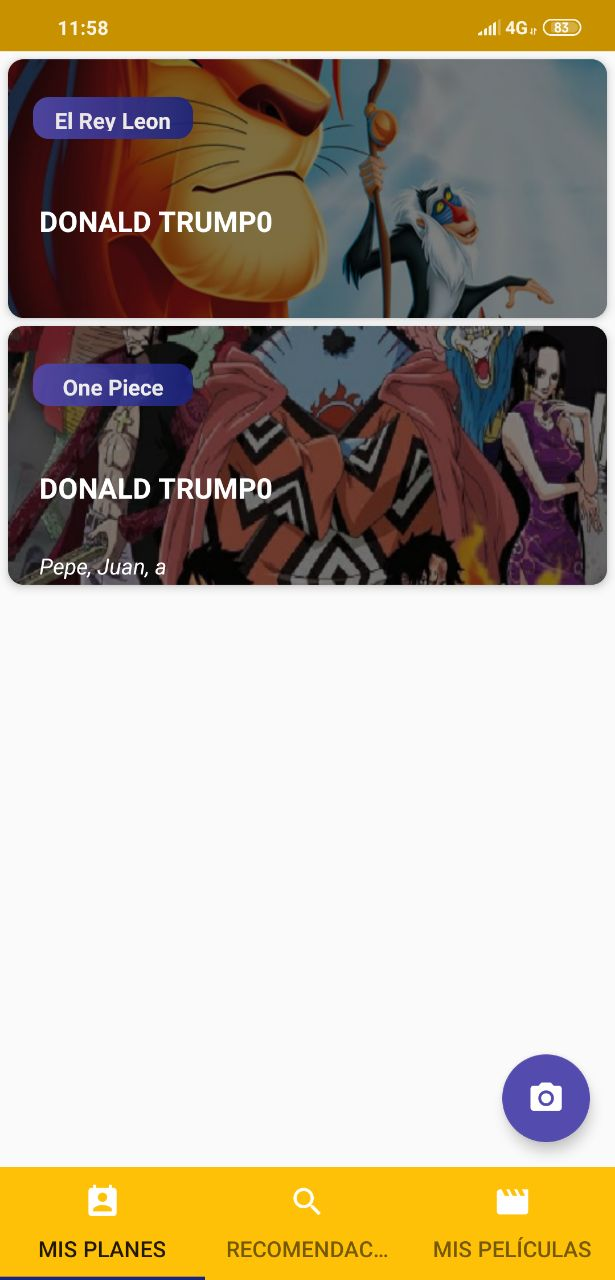
\includegraphics[width=3in]{figures/PlansList1.jpg}
    \caption{Lista de planes, primera versión}
\end{figure}
Podemos observar como cada elemento representa un plan, con el fondo siendo el cartel de la película, el título de la película en la esquina superior izquierda,
debajo el nombre del usuario que lo ha creado junto con las personas que se han unido al plan.
\\
Tras mostrarla en una de las reuniones con los directores de nuestro TFG, nos sugirieron cambiarla debido a que no reflejaba correctamente lo que era, es decir, 
cada plan no otorgaba la información suficiente a un usuario para que éste supiera que era un plan en sí. Por lo que posteriormente decidimos cambiar la vista
para mostrar al usuario la estructura de un plan correctamente y así ofrecerle una mejor experiencia de usuario. 
\\
La siguiente figura muestra la segunda versión de nuestra lista de planes: 
\begin{figure}[H]
    \centering
    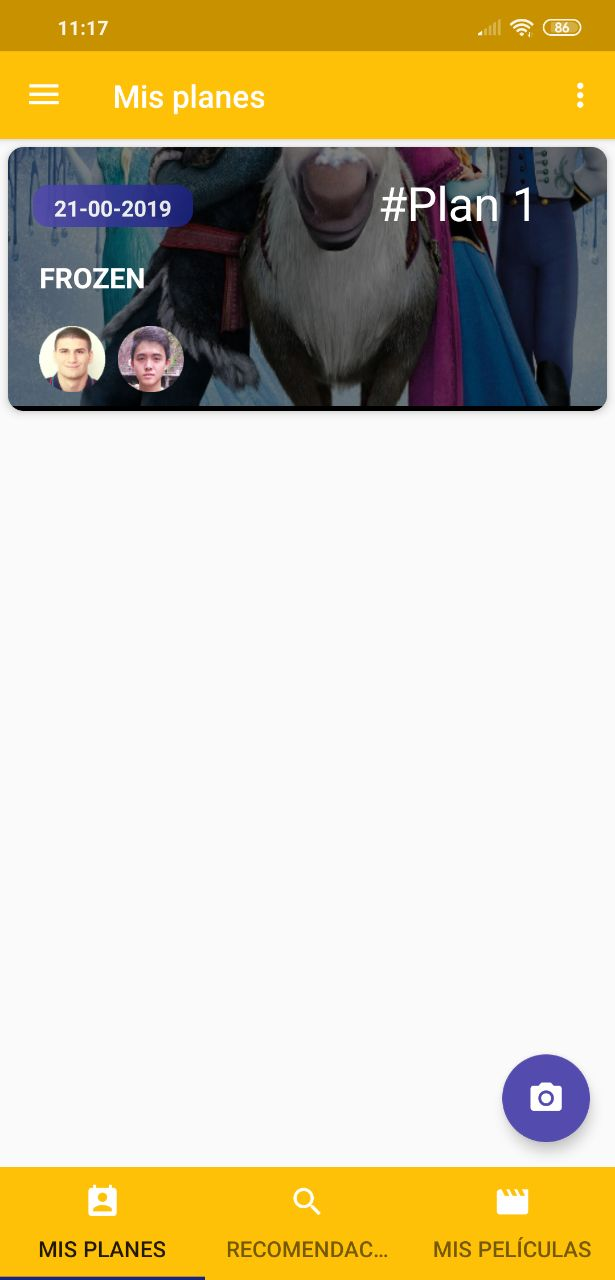
\includegraphics[width=3in]{figures/planslist2.jpg}
    \caption{Lista de planes, segunda versión}
\end{figure}
Podemos observar como ahora aparece la fecha para la que es el plan en la parte superior izquierda, justo debajo el título de la película que se quiere ver, arriba a la derecha el número del plan, algo simple pero que nos indica
claramente lo que representa este elemento.
El cambio más significativo es que, ahora en la parte inferior aparecen las fotos de los usuarios que se han unido al plan.
\subsection{Interfaz de lista de películas guardadas}
\label{makereference3.4.2}
Para mostrar las películas guardadas decidimos usar un grid que muestre solamente los carteles de las películas, es una interfaz simple pero muy visual, para acceder a la información
de cada película simplemente debemos pulsar en uno de los carteles.
\begin{figure}[H]
    \centering
    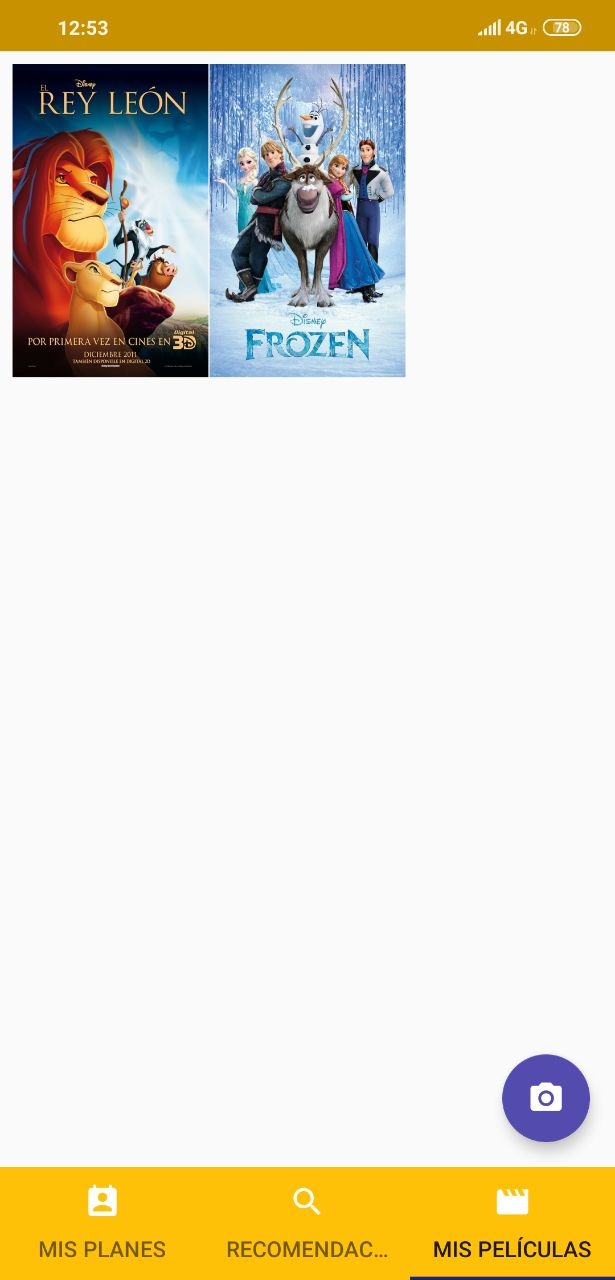
\includegraphics[height=5in]{figures/FilmsList.jpg}
    \caption{Lista de películas guardadas}
\end{figure}
En la figura 3.3 podemos observar que el usuario solo ha guardado 2 películas, si se guardaran más irían apareciendo al lado de las que ya están o pasarían debajo en cuanto una 
fila tuviera 3 elementos, elegimos este tamaño para que pudieran verse correctamente los carteles y los títulos de las películas.
\subsection{Interfaz principal}
\label{makereference3.4.3}
En la figura 3.3 también vemos como es la interfaz principal, con una barra en la parte inferior para movernos por las 3 secciones de nuestra aplicación: \textbf{mis planes}, \textbf{recomendaciones}, \textbf{mis películas}.
Cada sección incluye un icono para apoyar a la representación.
Además, encontramos un botón con un símbolo de una cámara en todas las secciones que nos permitirá acceder a la parte de \textbf{Realidad Aumentada}

\subsection{Interfaz de realidad aumentada al reconocer una película}
\label{makereference3.4.4}
En esta interfaz destacamos los distintos componentes que aparecen al usar la cámara de nuestro teléfono y reconocer el cartel de una película.
Lo primero que podemos observar al entrar a la interfaz de realidad aumentada es una especie de simulación de un escáner que se superpone a lo que vemos con la
cámara del teléfono, incitando así al usuario a reconocer algo con la cámara, esto lo podemos ver en la figura 3.4.

\begin{figure}[H]
    \centering
    
\includegraphics[width=3in]{figures/escaner.jpg}
    \caption{Escáner}
\end{figure}

Cuando reconocemos un cartel, sobre la imagen de la película nos aparecerá en la parte superior una valoración numérica de la película, la cual la hemos 
sacado de \textbf{IMDB}. justo en el medio de la imagen encontramos el icono típico de \textbf{Youtube} que, al pulsarlo, nos abrirá nuestra aplicación de \textbf{Youtube} para que
el usuario pueda ver el tráiler de esta película. En la esquina inferior derecha encontramos otro icono que al ser pulsado lo que hará será desplegar una serie de botones con distinta funcionalidad,
uno de ellos nos redirige a la información de la película en \textbf{IMDB}, que sería el icono representado por una letra \textbf{i}, el otro botón representado por una mano con un pulgar hacia arriba nos permitirá
guardar la película en nuestra lista de películas guardadas, para posteriormente acceder a su información, valorarla o crear un plan con ella. Todo esto lo podemos observar en la figura 3.5 y 3.6.
\begin{figure}[H]
    \centering
    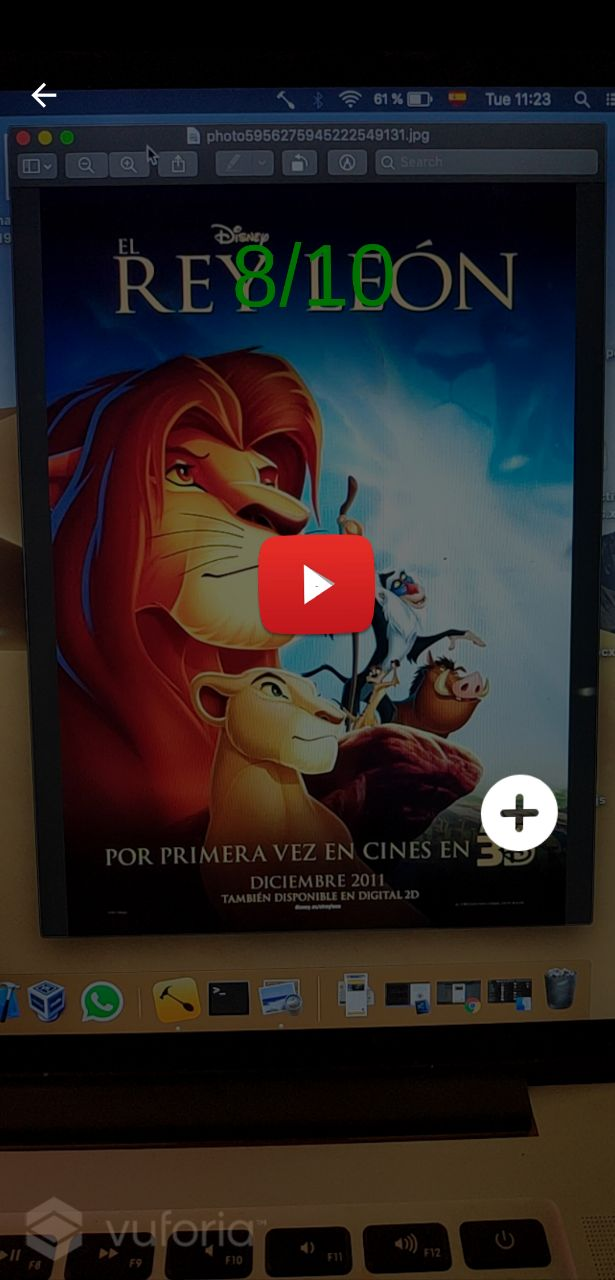
\includegraphics[width=3in]{figures/filmrecognized1.jpg}
    \caption{Realidad aumentada tras reconocer una película}
\end{figure}
\begin{figure}[H]
    \centering
    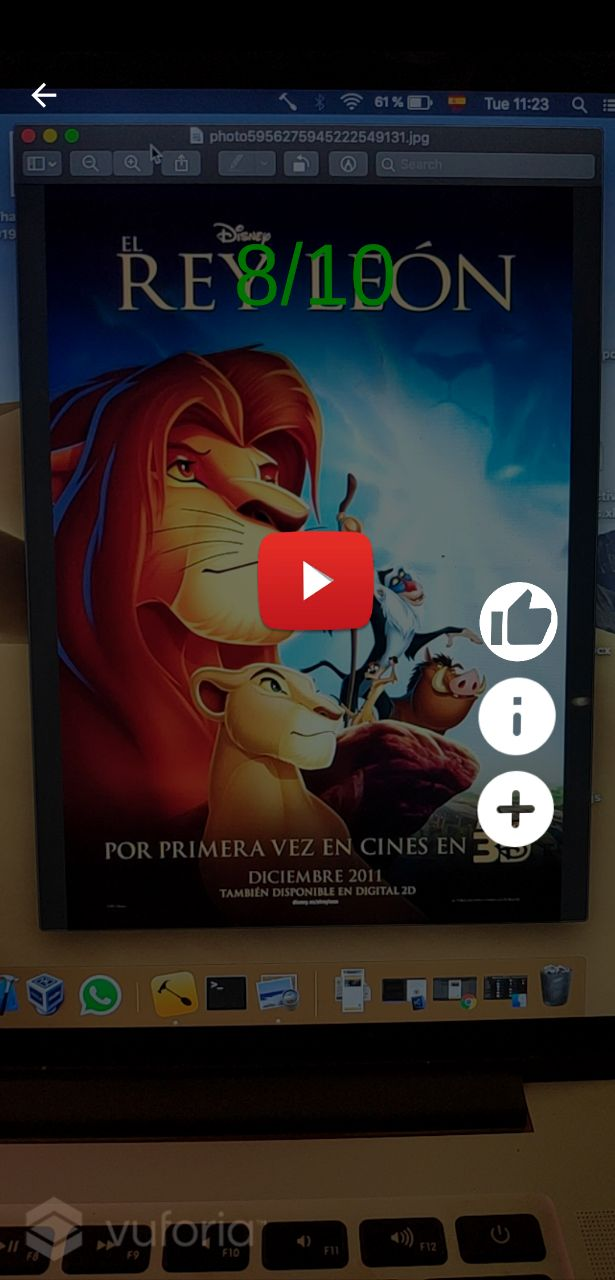
\includegraphics[width=3in]{figures/filmrecognized2.jpg}
    \caption{Realidad aumentada tras reconocer una película}
\end{figure}

\newpage
\subsection{Interfaz de realidad aumentada al reconocer a un usuario}
\label{makereference3.4.5}
\begin{flushleft}
Cuando reconocemos a un usuario de la aplicación con la cámara de nuestro dispositivo se pueden dar dos casos,
 que sea amigo del usuario que lo está reconociendo o que todavía no lo sea.
\end{flushleft}
\begin{flushleft}
Si no es un amigo aparecerá una interfaz para añadir al usuario como amigo, mientras que si es un amigo 
aparecerá una interfaz distinta en donde el usuario puede incorporarse a los planes de su amigo.
\end{flushleft}
\subsection{Interfaz de realidad aumentada al reconocer a un usuario que no es amigo}
\label{makereference3.4.5.1}
\begin{flushleft}
Se trata de una interfaz sencilla en donde al usuario que enfoca se le proporciona el nombre del usuario al
 que está enfocando (siempre que el usuario enfocado esté registrado) junto a un botón de añadir amigo.
\end{flushleft}
\subsection{Interfaz de realidad aumentada al reconocer a un usuario que sí es amigo}
\label{makereference3.4.5.2}
\begin{flushleft}
Esta interfaz que aparece al enfocar con la cámara a un usuario que es amigo del que enfoca, es una interfaz
 más compleja que la anteriormente descrita.
\end{flushleft}
\begin{flushleft}
Cuando un usuario enfoca a otro que es amigo, se proporciona la opción de incorporarse a uno de los planes del
 amigo. Para ello, se le muestra una interfaz con los tres planes que según nuestro algoritmo de recomendación
  más pueden interesarle de los que su amigo tiene.
\end{flushleft}
\begin{flushleft}
La interfaz proporciona la imagen de las películas de los tres planes, además, mediante una interfaz dinámica 
podemos movernos de un plan a otro, de esta forma podemos ver quien hay en el plan junto a la puntuación que 
nuestro sistema de recomendación calcula que le gusta a cada participante el plan.
\end{flushleft}
\begin{figure}[H]
        \centering
        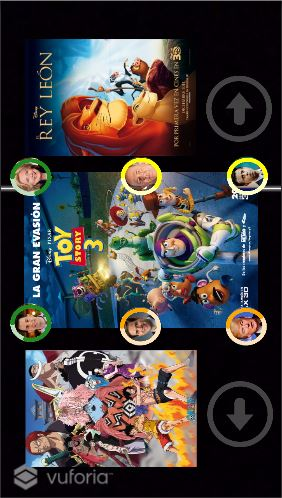
\includegraphics[width=3in, angle=270]{figures/chapter-2/recomendadorAR.JPG}
        \caption{Vista encargada de recomendar planes en RA al enfocar a un amigo}
\end{figure}
\begin{flushleft}
Como se puede ver en la figura 3.20, en la interfaz aparecen las tres películas, únicamente se muestra la 
información relacionada con los usuarios del plan situado en medio para no saturar la interfaz. Mediante los 
botones de izquierda y derecha el usuario puede moverse entre planes para poder ver la información necesaria 
de cada plan y elegir aquel que más le guste.
\end{flushleft}
\begin{flushleft}
La información visual que aparece relacionada con los usuarios representa:
\begin{itemize}
    \item Arriba a la izquierda el amigo que se encuentra ya en el plan junto con una representación gráfica 
    de cuanto estima el algoritmo de recomendación que le puede gustar la película.
    \item Arriba a la derecha, la foto del usuario que está valorando unirse al plan junto con una representación 
    gráfica de cuanto estima el algoritmo de recomendación que le puede gustar la película.
    \item El resto de las posiciones identifican al resto de usuarios junto con la representación gráfica de 
    cuanto se estima que le puede gustar la película.
    
\end{itemize}
\end{flushleft}

\subsection{Interfaz de inicio de sesión y de registro}
\label{makereference3.4.6}

Nos aparecerá una interfaz muy simple para realizar el inicio de sesión con un usuario en la aplicación al entrar. También nos permite registrarnos como usuarios si
aún no poseemos una cuenta en la aplicación.

\begin{figure}[H]
    \centering
    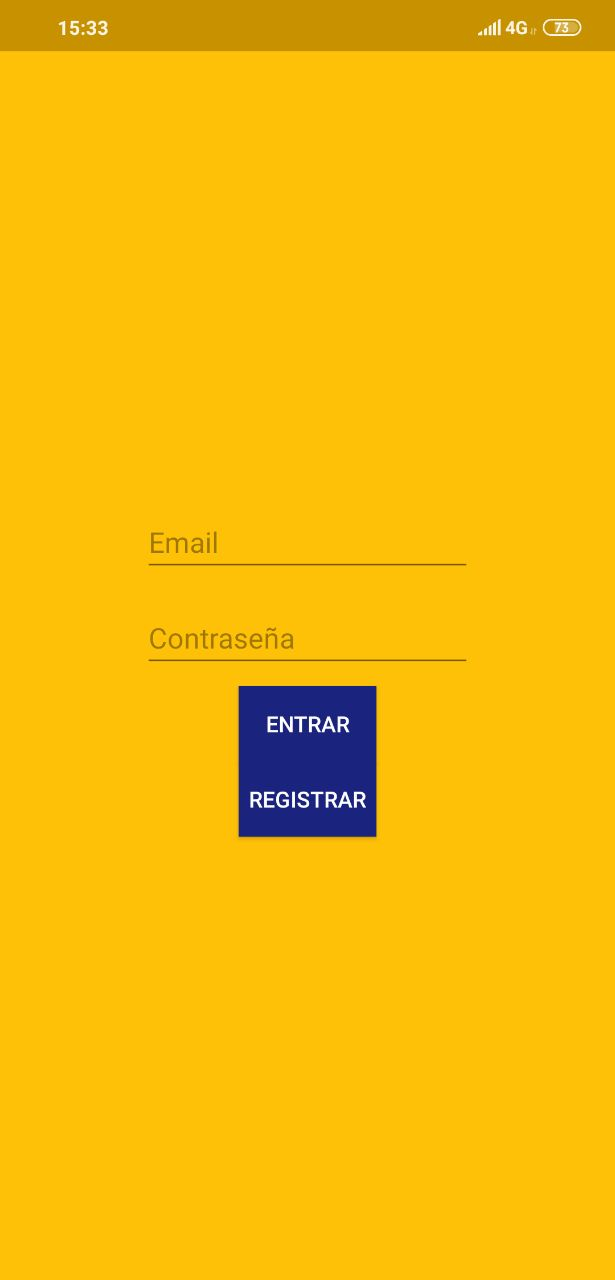
\includegraphics[height=4in]{figures/login.jpg}
    \caption{Inicio de sesión}
\end{figure}
\begin{figure}[H]
    \centering
    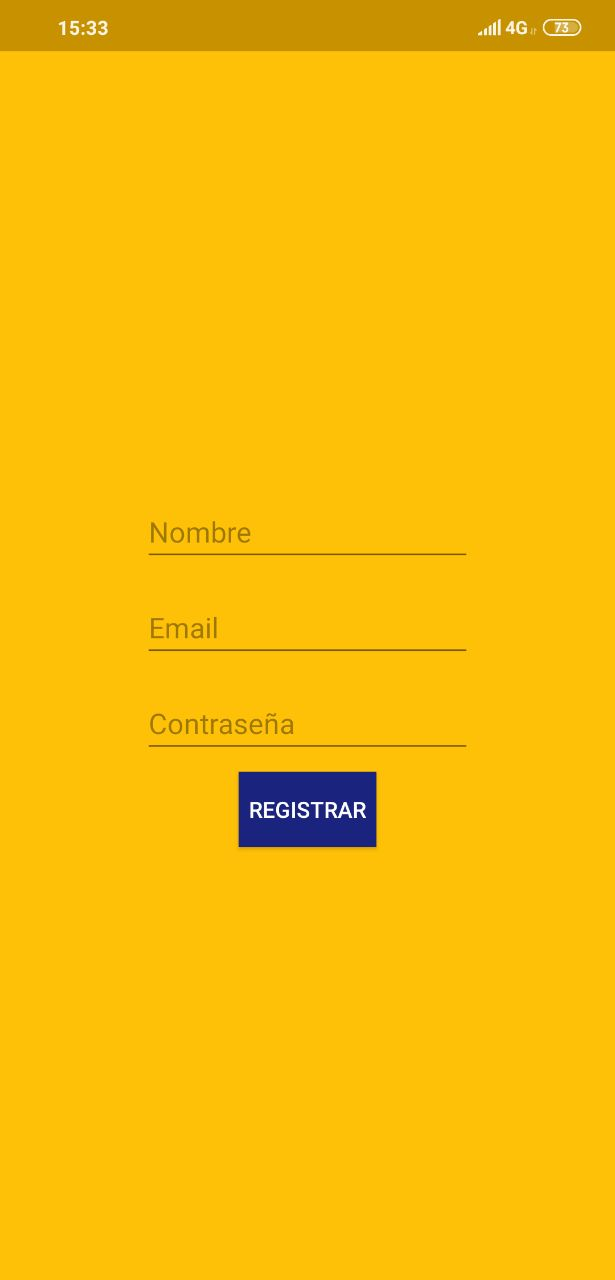
\includegraphics[height=4in]{figures/register.jpg}
    \caption{Registro}
\end{figure}

\subsection{Interfaz de recomendaciones}
\label{makereference3.4.7}

\subsection{Interfaz de información de una película}
\label{makereference3.4.8}

Tras pulsar en una de las películas que hemos guardado nos aparecerá dicha interfaz. 
Esta vista nos permite ver en primer plano el cartel de la película y la información correspondiente a la misma, como puede
ser la sinopsis de la película, el género y el nombre del director. Además, poseemos un \textbf{Gauge} que nos permite, al pulsarlo,
valorar la película mediante una barra de progreso.
Si hacemos scroll hacia abajo, la imagen de la película se irá ocultando para ofrecernos una mejor visión de la información de la película.
En la parte inferior se nos presentan dos botones, uno para crear un plan con la película, que es el de color amarillo con el texto: \textbf{AÑADIR AL PLAN}. El otro botón de color
violeta con el símbolo de reproducir un vídeo, nos llevará al trailer de la película en \textbf{Youtube}.
Arriba a la derecha observamos el icono de un corazón, lo que nos permitirá quitar esta película de nuestras favoritas y ya no aparecerá en la
lista de películas guardadas.

\begin{figure}[H]
    \centering
    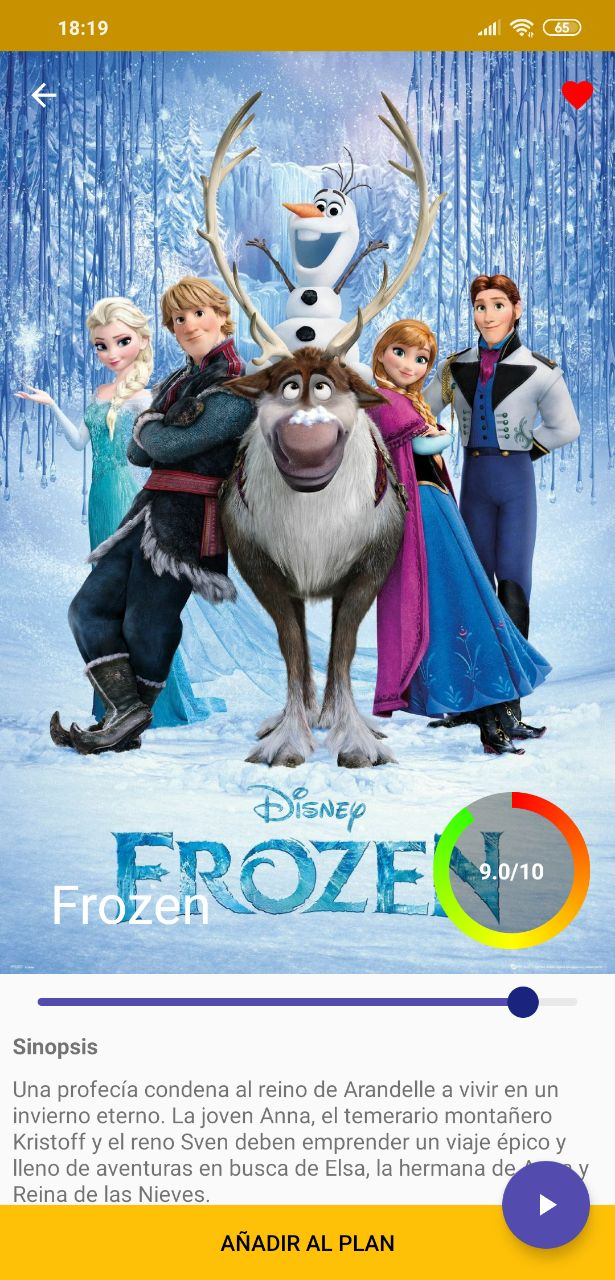
\includegraphics[width=3in]{figures/infoFilm1.jpg}
    \caption{Información de la película}
\end{figure}
\begin{figure}[H]
    \centering
    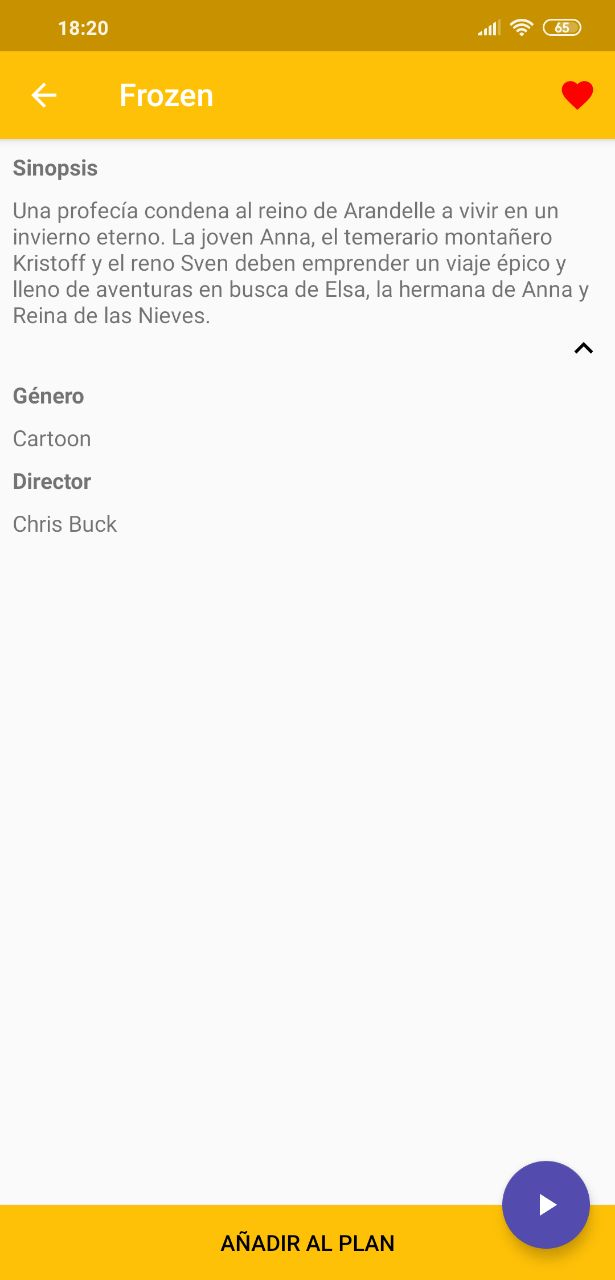
\includegraphics[width=3in]{figures/infoFilm2.jpg}
    \caption{Información de la película observando el cambio en el Gauge tras valorar}
\end{figure}
\begin{figure}[H]
    \centering
    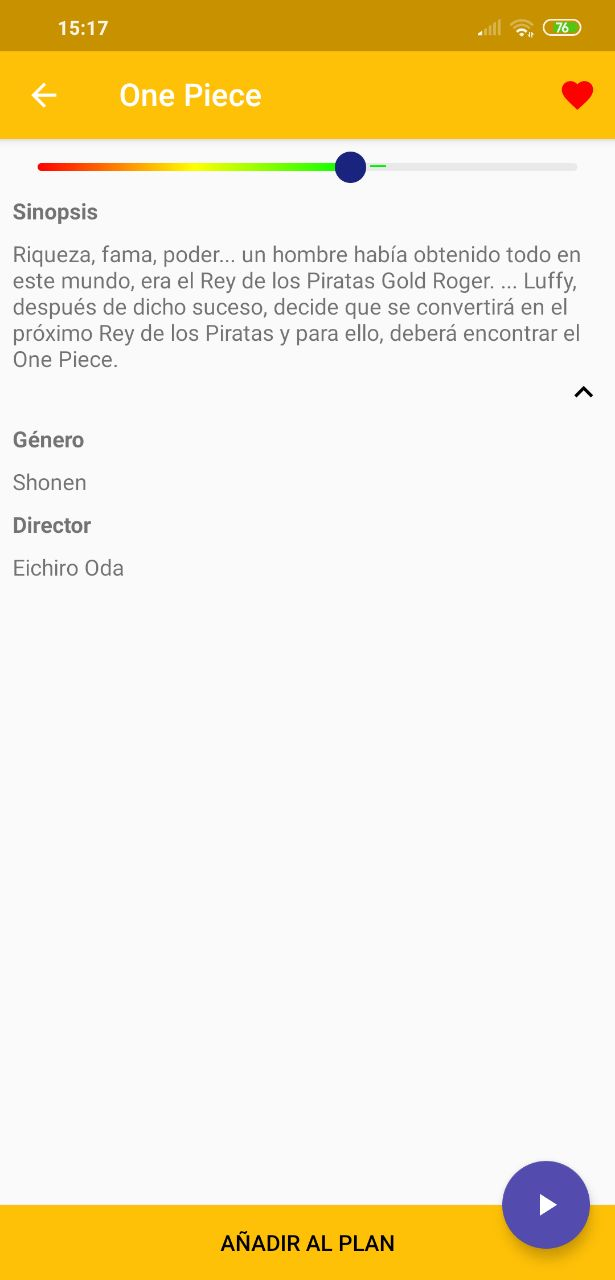
\includegraphics[width=3in]{figures/infoFilm3.jpg}
    \caption{Información de la película cuando se hace el scroll hacia abajo}
\end{figure}

\subsection{Interfaz de información de un plan}
\label{makereference3.4.9}
Esta interfaz aparece cuando pulsamos en un plan y es muy similar a la que se le muestra al usuario con la información
de una película. También nos aparecerá en grande la imagen de la película que se quiere ir a ver con dicho plan, junto con información
relevante de dicho plan, como puede ser:
\begin{itemize}
    \item \textbf{Fecha}: día, mes y año en el que tendrá lugar dicho plan.
    \item \textbf{Hora}: hora del plan.
    \item \textbf{Lugar}: localización que haya puesto el creador del plan para ver la película.
    \item \textbf{Descripción}: breves anotaciones características que haya escrito el creador sobre el plan.
    \item \textbf{Usuarios unidos}: imágenes de los usuarios que se han unido al plan.
\end{itemize}
Además, nos aparece un botón en la parte inferior con el texto: \textbf{UNIRSE AL PLAN} o \textbf{SALIR DEL PLAN}, según estemos o no ya dentro del plan.
También en la parte inferior derecha de la imagen de la película tenemos un botón que nos redirige a la interfaz de información de dicha película.
En la parte superior derecha nos aparece un icono de una basura, lo que nos permitirá borrar el plan, si somos el creador.
\begin{figure}[H]
    \centering
    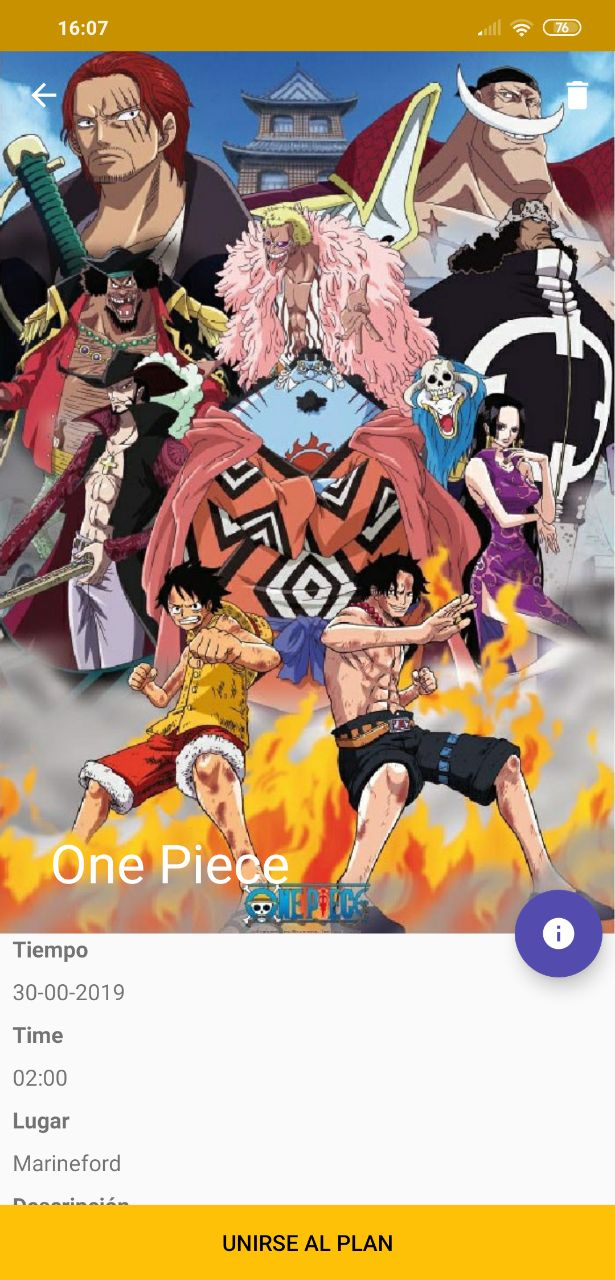
\includegraphics[width=3in]{figures/infoPlan1.jpg}
    \caption{Información del plan}
\end{figure}
\begin{figure}[H]
    \centering
    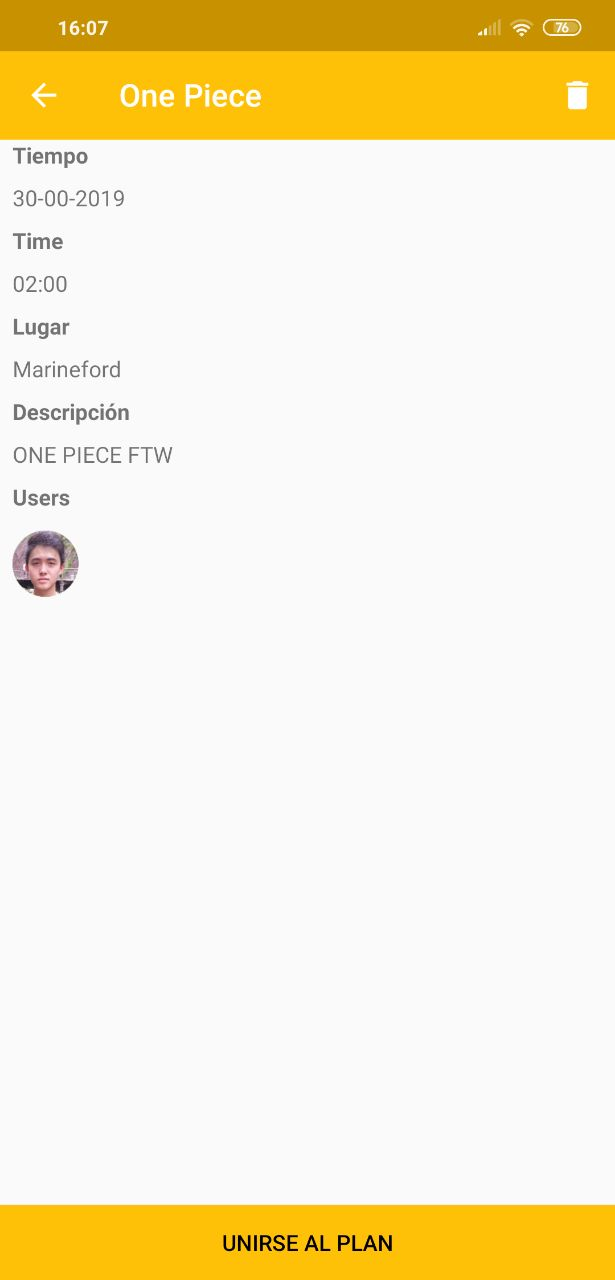
\includegraphics[width=3in]{figures/infoPlan2.jpg}
    \caption{Información del plan tras hacer el scroll hacia abajo}
\end{figure}
% +--------------------------------------------------------------------+
% | Sample Chapter 4
% +--------------------------------------------------------------------+

\cleardoublepage

% +--------------------------------------------------------------------+
% | Replace "This is Chapter 4" below with the title of your chapter.
% | LaTeX will automatically number the chapters.
% +--------------------------------------------------------------------+

\chapter{Implementación}
\label{makereference4}
Nuestra aplicación es una aplicación móvil desarrollada en Android, Unity y Vuforia y con un servidor desarrollado en Java usando Spring.
En este capítulo comenzaremos describiendo todos los prototipos de implementación que hemos desarrollado, en los cuáles veremos los pros y contras de las
tecnologías que hemos probado y el porqué de nuestra elección de implementar la aplicación con estas tecnologías. 
Después describiremos cómo hemos implementado nuestra aplicación, desde la arquitectura que hemos seguido, 
las tecnologías usadas para la parte frontend y la parte backend junto a las dificultades 
que nos hemos encontrado mientras trabajábamos. Finalmente hablaremos de las herramientas de trabajo
utilizadas para facilitarnos el trabajo en equipo.
\begin{center}
    \begin{tabularx}{1\textwidth}{@{\extracolsep{\fill}} | X | l | l |} \hline
    \multicolumn{3}{|l|}{Enlaces de GitHub } \\ \hline
    Aplicación & Licencia & Enlace \\ \hline
    Escena de AR en Unity con Vuforia & Apache-2.0 & \url{https://github.com/DanielCalle/TFG-Vuforia} \\ \hline
    Aplicación de Android & Apache-2.0 & \url{https://github.com/DanielCalle/TFG-Android} \\ \hline
    Servidor de Spring & Apache-2.0 & \url{https://github.com/DanielCalle/TFG-Server} \\ \hline
    \end{tabularx}
\end{center}
\section{Pruebas de arquitectura}
\label{makereference4.1}
Estas pruebas sirven para conocer si las tecnologías seleccionadas
de la \autoref{makereference2.1.1} son viables dentro de nuestro proyecto.
Desarrollaremos prototipos con funcionalidades básicas y evaluaremos las partes
positivas y negativas de dichas tecnologías. Esto nos permitirá decidir cuales
son las mejores opciones para construir el software.

\subsection{ARCore} 
\label{makereference4.1.1} 
    Al comenzar la fase de desarrollo de proyectos, pensamos que una de las tecnologías que debíamos 
    investigar y probar debía ser ARCore. Esto se debía a que, la empresa detrás de esta 
    tecnología es Google y esto podría significar que tendríamos más material de consulta 
    y ejemplos en comparación con otras tecnologías de fabricantes con menos recursos.
    ARCore se encuentra disponible para Java, Unity, Unreal e iOS. Comenzamos realizando el 
    "Quickstart"\ para Android y posteriormente para Unity. 
    Tras realizar los proyectos propuestos por ARCore, realizamos algún proyecto propio 
    para comprobar si la herramienta se ajustaba a la idea que teníamos para nuestro futuro proyecto.
    Tras realizar ambos proyectos, concluimos que, aunque ARCore reúne las características 
    necesarias para en un futuro convertirse en una de las tecnologías más importantes en Realidad Aumentada, 
    no íbamos a seleccionarla para nuestro proyecto por las siguientes razones:
    \begin{itemize}
        \item Dispone de mucha documentación para comenzar a usar la herramienta, pero poca para realizar tareas más complejas.
        \item Resulta muy útil para realizar superposiciones de modelos 3D sobre superficies. Sin embargo, una de las funcionalidades más importantes que nuestra aplicación requería era la interacción con la realidad aumentada mediante el uso de botones, imágenes y la carga dinámica de elementos para posicionar en la pantalla de Realidad Aumentada e interaccionar con el usuario. En este sentido ARCore no está, por el momento, tan preparada como otras tecnologías.
    \end{itemize}
\subsection{Viro Media} 
\label{makereference4.1.2}

El objetivo del prototipo realizado con Viro Media es reconocer imágenes almacenadas en el dispositivo para mostrar texto y
objetos virtuales. Además de probar tecnologías de desarrollo móvil web como en este caso React Native
para plataformas iOS y Android. Comenzamos construyendo una interfaz sencilla con botones que nos redirigen a la escena de Realidad Aumentada (ver \autoref{fig:nativeBase_android} y \autoref{fig:nativeBase_ios}).
Para esta interfaz utilizamos NativeBase que es una librería que nos permite
realizar una aplicación con apariencias de tipo iOS o Android según el dispositivo.

\begin{figure}[htb]
    \centering
    \makebox[0pt][c]{%
    \begin{minipage}[b]{0.5\linewidth}
    \centering
      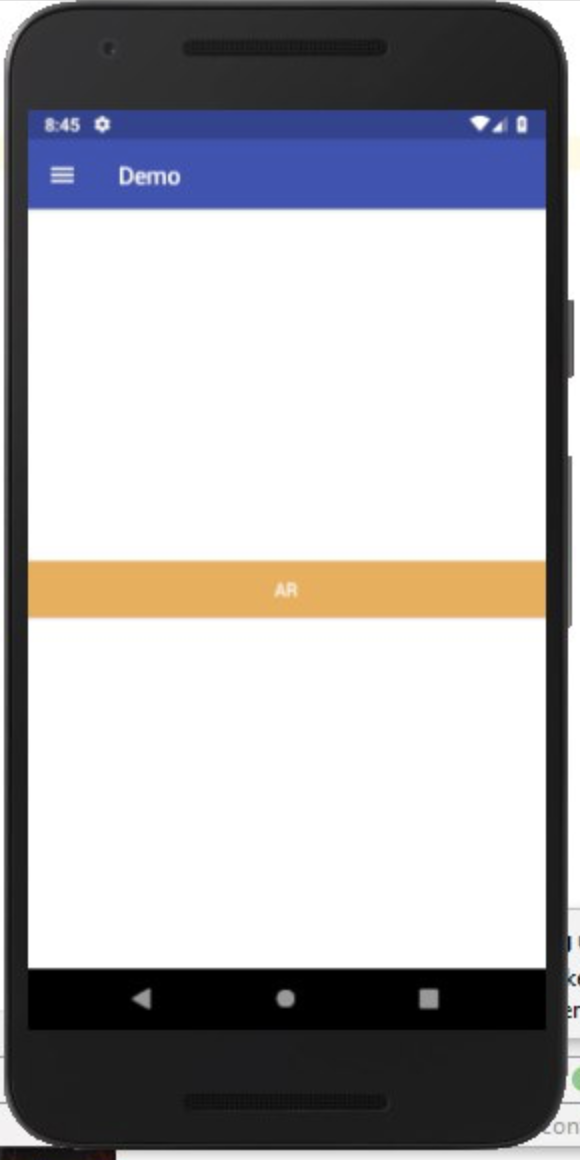
\includegraphics[scale=0.3]{figures/chapter-3/viromedia/android.png}
      \caption{Visualización con NativeBase en Android}
    \label{fig:nativeBase_android}
    \end{minipage}%
    \hspace{0.3cm}
    \begin{minipage}[b]{0.5\linewidth}
    \centering
     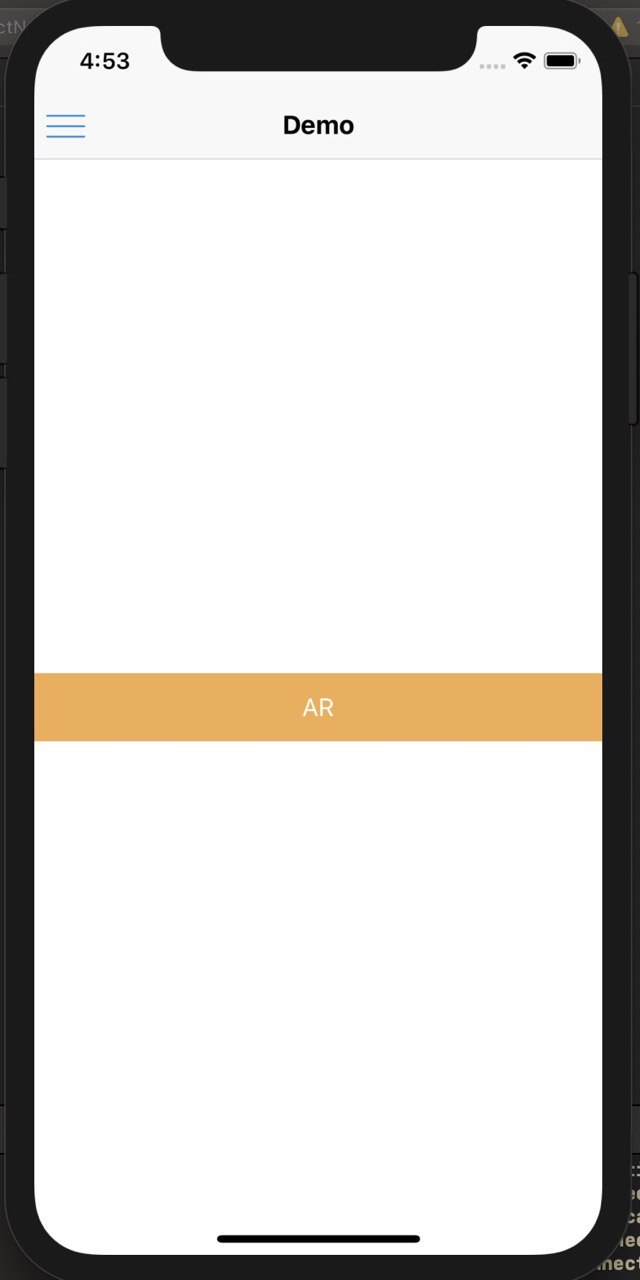
\includegraphics[scale=0.3]{figures/chapter-3/viromedia/ios.jpg}
      \caption{Visualización con NativeBase en iOS}
    \label{fig:nativeBase_ios}
    \end{minipage}%
    }%
\end{figure}

Para la escena de realidad aumentada mostramos texto y al detectar el póster de Pantera Negra,
reacciona mostrando una animación de dicho superhéroe saliendo del póster (ver \autoref{fig:visualizacionRANAtibe}).
 
\begin{figure}[H]
    \centering
    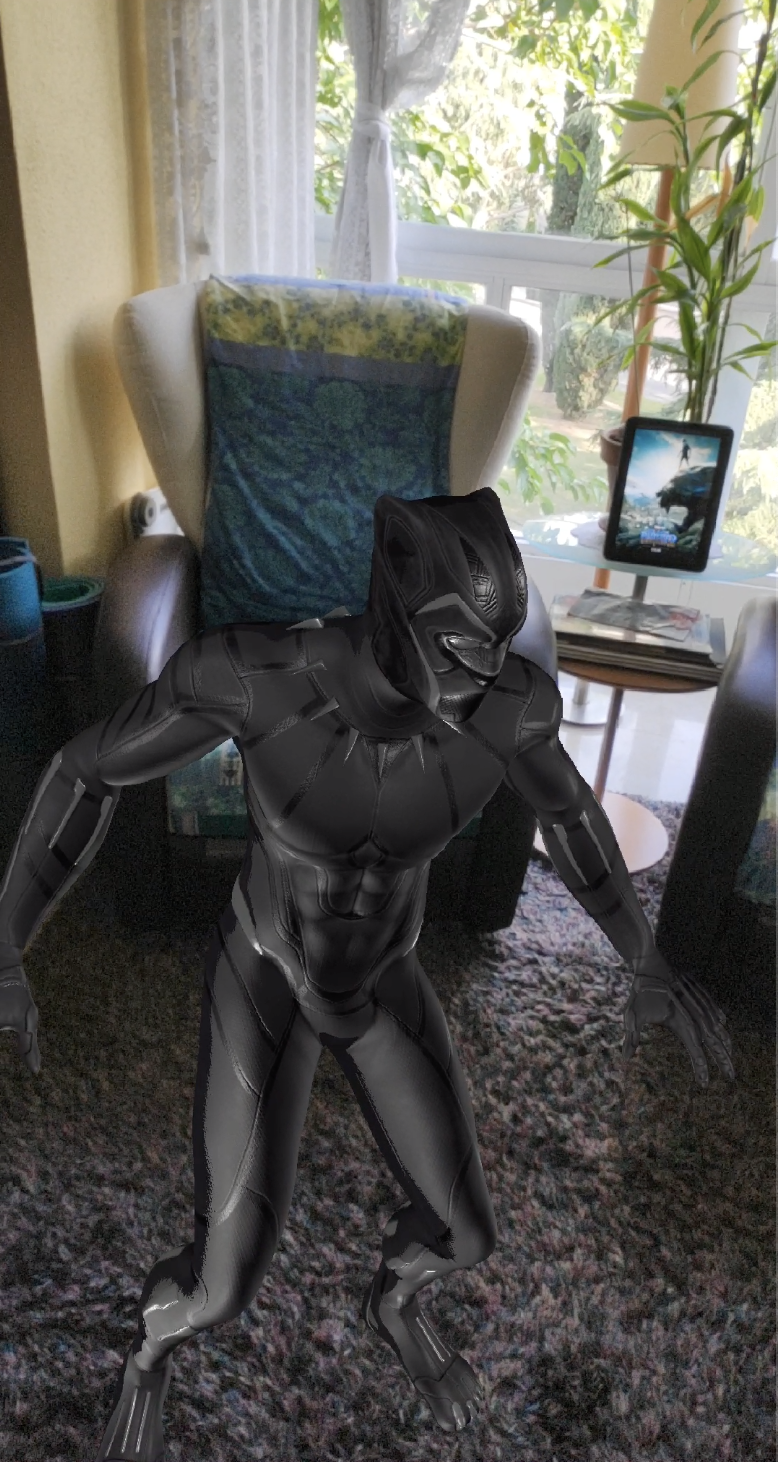
\includegraphics[height=4in]{figures/chapter-3/viromedia/blackpanther.png}
    \caption{Visualización de RA}
    \label{fig:visualizacionRANAtibe}
\end{figure}
\newpage
Una de las ventajas que apreciamos fue la facilidad del lenguaje, en este caso Javascript,
 utilizando la popular librería ReactJS y la buena documentación de Viro Media
 que hacían que el proceso de codificación fuera agradable.\\

Uno de los problemas que presentaba este prototipo era que las dependencias de Viro Media entraban en conflicto con las de NativeBase
imposibilitándonos la forma de encontrar versiones compatibles. Utilizamos las últimas que, a pesar de lanzar
 advertencias, funcionaba en el ejemplo realizado.
Otro problema fue la compilación de la aplicación, Viro Media tiene una aplicación para probar lo
 que desarrollamos conectándose a nuestro ordenador a través de la red. El problema es
 que algunos recursos, como los iconos que utilizaba NativeBase, no eran descargados, por lo que la
 mejor forma era probar la versión compilada de iOS y Android. La forma de compilar
 la aplicación era un proceso costoso para los ordenadores, lento y con multitud de problemas según
 se ampliaban las librerías que se utilizan.\\

La conclusión que obtuvimos de este prototipo fue que Viro Media y React Native son tecnologías muy prometedoras, pero debido a los
 problemas surgidos y a que todas sus versiones no eran estables vimos un claro riesgo para

\subsection{Vuforia + Android} 
\label{makereference4.1.3} 
 
En este prototipo utilizamos la librería nativa de Vuforia para Android para 
realizar las pruebas de tecnología de reconocimiento de imágenes tanto en  
local como usando la nube que nos ofrecía Vuforia, para la posterior renderización
de objetos y textos.

Las características tecnológicas de este prototipo son las siguientes:


\begin{enumerate}
    \item La librería de Vuforia para Android está diseñada a muy bajo nivel.
    \item Vuforia para dibujar en 3D usa la librería OpenGL (ver \autoref{fig:modelo3D}).
    \item OpenGL utiliza una serie de espacios donde se van colocando los elementos (ver \autoref{fig:esquemaOpenGl}): 
    \begin{enumerate}
        \item Local space: Es el espacio local de cada objeto.
        \item World space: Es el mundo donde se encuentran los objetos.
        \item View space: El mundo visto desde la perspectiva de la cámara.
        \item Clip space: Se integra con la pantalla del móvil y, definiendo los límites visibles, se establecen unas coordenadas de rango (-1,-1) - (1,1).
    \end{enumerate}
    
        Las transformaciones de estos espacios se realizan mediante matrices 4x4, 
        en las que la primera fila hace referencia a la coordenada $x$, la segunda a la coordenada $y$ y la 
        tercera a la coordenada $z$, mientras que la última columna hace referencia a los desplazamientos 
        de los objetos en esos 3 ejes.
            \begin{figure}[H]
                \centering
                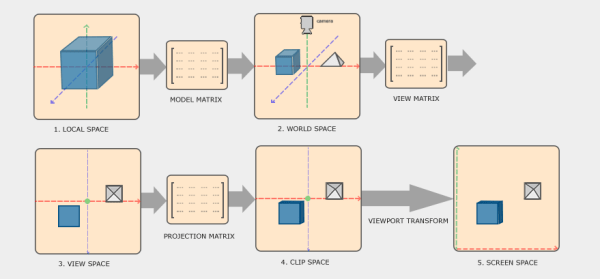
\includegraphics[width=5in]{figures/space-transformation.png}
                \caption{Esquema de los distintos espacios que usa OpenGL\cite{spaceopengl}}
                \label{fig:esquemaOpenGl}
            \end{figure}


            \begin{figure}[H]
                \centering
                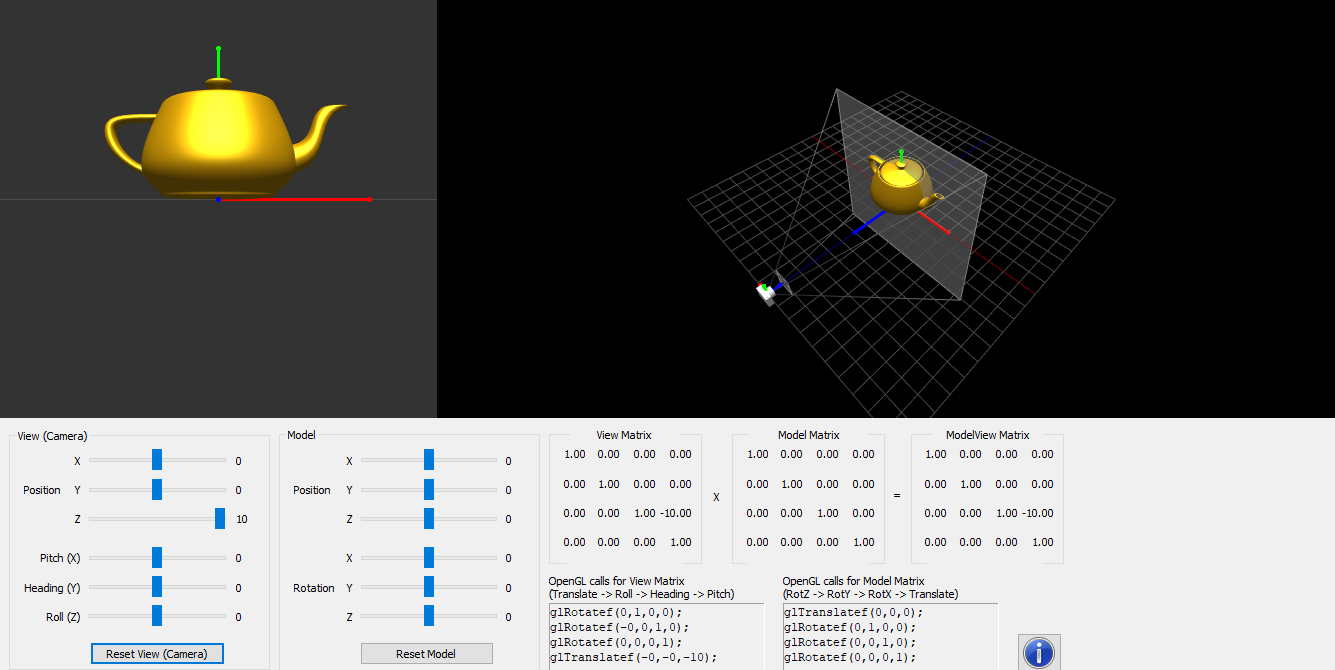
\includegraphics[width=5in]{figures/teapot.png}
                \caption{Captura de un ejemplo de un modelo en 3D}
                \label{fig:modelo3D}
            \end{figure}

    
    \item En OpenGL es necesario escribir código para que las tarjetas gráficas rendericen el modelo 3D,
    el lenguaje que se usa es GLSL. Este código de GLSL se escribe en forma de String y se llama a un método 
    que proporciona OpenGL, podemos ver un ejemplo de este código en la \autoref{fig:codigoGLSL}.
    \begin{figure}[H]
        \centering
        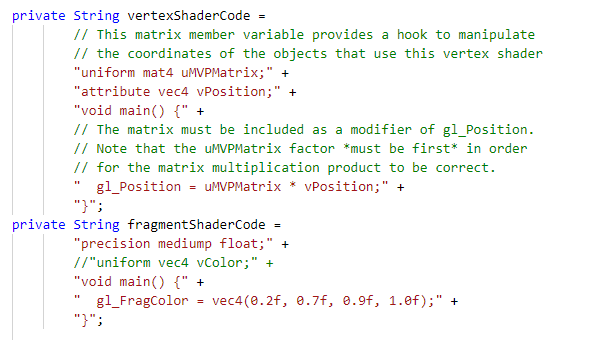
\includegraphics[width=5in]{figures/GLSL.png}
        \caption{Código en GLSL}
        \label{fig:codigoGLSL}
    \end{figure}
    \newpage    
    \item Otro aspecto a tener en cuenta es que OpenGL solo nos ofrece lo básico, no nos ofrece métodos para dibujar 
    directamente objetos, sino que hay que seguir un pipeline de procesos para conseguir dibujar algo (ver \autoref{fig:pipeline}).
    Esto consiste en pasar un array de números (cada tres para definir un punto) 
    a las tarjetas gráficas, establecer triángulos entre los puntos (más arrays de números) 
    definir colores a partir de los puntos (más arrays...), y con el código del shader, ejecutar 
    estos datos.
    \begin{figure}
        \centering
        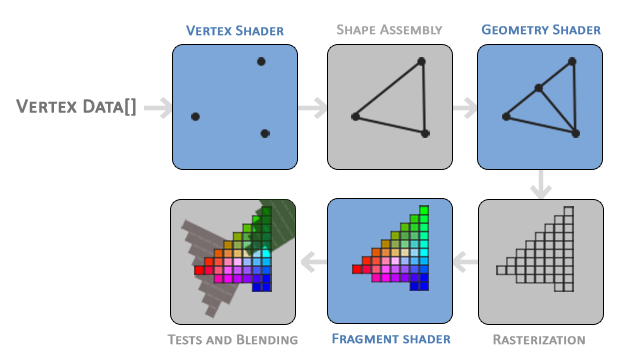
\includegraphics[width=4in]{figures/pipeline.png}
        \caption{Pipeline de la construcción de un modelo\cite{pipelineopengl}}
        \label{fig:pipeline}
    \end{figure}
    \item Por último, como sólo ofrece métodos básicos, no hay métodos de escritura de texto, y la forma que 
    encontramos para que funcione fue usar un bitmap con los caracteres (ver \autoref{fig:mapaBits}). Este fue el principal 
    motivo de rechazar esta tecnología ya que, dependiendo de la funcionalidad que se desee implementar, es necesario codificar a muy bajo nivel, lo que costaría mucho tiempo y esfuerzo.
    \begin{figure}
        \centering
        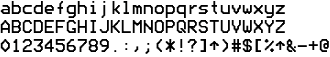
\includegraphics[width=5in]{figures/bitmap-font.png}
        \caption{Mapa de bits de caracteres usado}
        \label{fig:mapaBits}
    \end{figure}
\end{enumerate}

\subsection{Vuforia + Unity} 
\label{makereference4.1.4}

    Para realizar este prototipo utilizamos Unity como herramienta básica para realizar la aplicación y Vuforia para dar soporte a la realidad aumentada.
    El prototipo a desarrollar consistió en un modelo 3D de un dragón que aparecía al detectar una imagen que previamente habíamos establecido como ``imagen objetivo''.

    \begin{figure}[H]
        \centering
        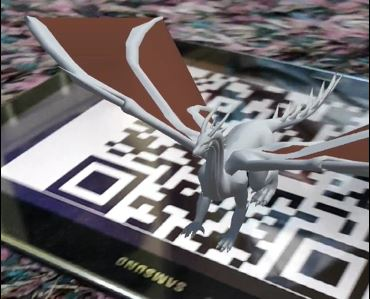
\includegraphics[width=5in]{figures/prototipoUnity.jpg}
        \caption{Modelo en 3D que aparecía al detectar la imagen}
    \end{figure}

Pese a que nadie del equipo había utilizado Unity previamente el resultado fue bastante positivo ya que:
\begin{enumerate}
    \item Unity resultó ser intuitivo y relativamente fácil en cuanto al aprendizaje de las funcionalidades básicas.
    \item Vuforia parecía estar muy probada e incluía de serie muchas funcionalidades.
    \item Vuforia tenía la opción de utilizar un Cloud para almacenar las imágenes objetivo.
\end{enumerate}


\subsection{Vuforia + Unity + Android} 
\label{makereference4.1.5}

Una vez realizado el prototipo en Vuforia con Unity comenzamos a investigar cómo realizar el resto de la aplicación que no requería de Realidad Aumentada.
Hasta este momento teníamos claro que Vuforia con Unity era la mejor combinación para realizar la parte de realidad aumentada. Sin embargo, tras realizar pruebas desarrollando en Unity interfaces y lógica nos dimos cuenta de que Unity no era igual de intuitivo ni eficaz a la hora de realizar estas tareas que necesitábamos para desarrollar el resto de la aplicación que no necesitaba Realidad Aumentada.
Por este motivo intentamos buscar la opción de realizar una aplicación en la que la realidad aumentada estuviese diseñada en Unity con Vuforia y el resto de la aplicación en Android (ver \autoref{fig:botonAndroidUnity}).

\begin{figure}[H]
    \centering
    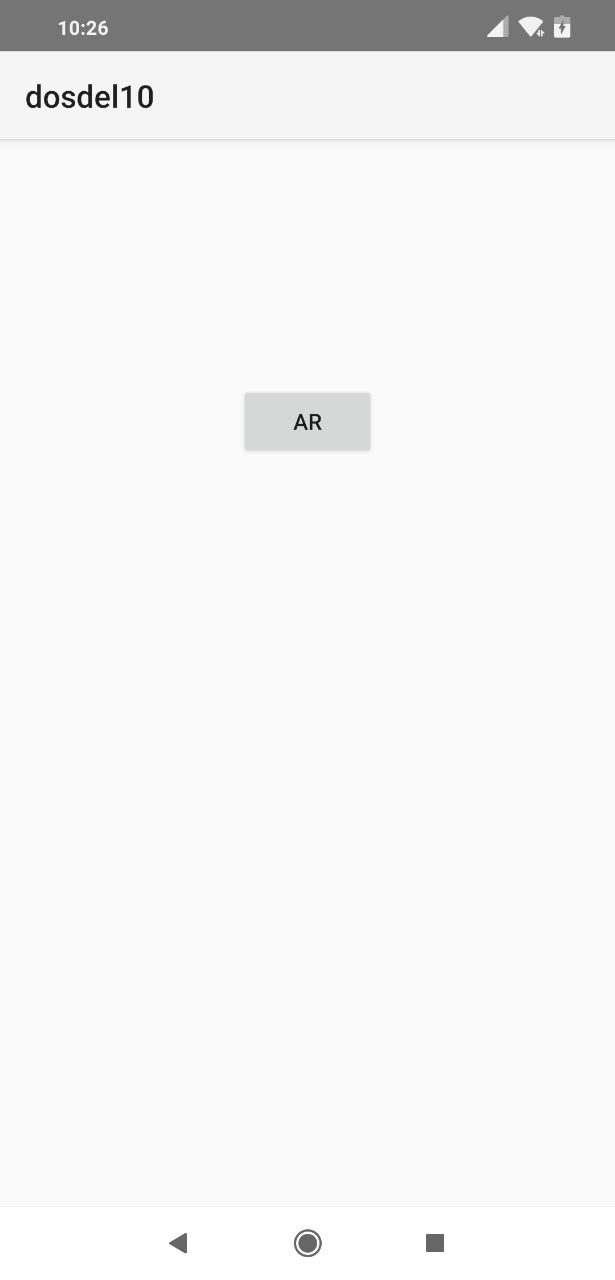
\includegraphics[height=4in]{figures/androidUnityVuforia.jpg}
    \caption{Botón que comunica Android con Unity}
    \label{fig:botonAndroidUnity}
\end{figure}

Finalmente conseguimos tener ambos proyectos independientes. La realidad aumentada se desarrollaba en Unity con Vuforia y se exportaba a un proyecto Android donde se encontraba el resto de la aplicación.
Esto nos permitía realizar la realidad aumentada con la herramienta que tras las primeras tomas de contacto habíamos comprobado que era la mejor (Unity con Vuforia) y del mismo modo realizar el resto de la aplicación con la mejor herramienta para esta parte (Android Studio).

Tras realizar este prototipo, consideramos que estas herramientas podrían ser las que usásemos en la aplicación final puesto que:
\begin{enumerate}
    \item Como ya habíamos descubierto en el prototipo anterior, Unity era una herramienta muy completa y junto con Vuforia nos proporcionaban todas las herramientas necesarias para cumplir con los casos de uso de Realidad Aumentada que teníamos en mente.
    \item Al haber encontrado la forma de combinar Unity y Android no teníamos que renunciar a ninguna de las dos herramientas. Lo que nos permitía explotar las cosas buenas de ambas herramientas.
    \item La comunicación entre Unity y Android era relativamente sencilla pese a ser dos proyectos distintos.
\end{enumerate}


\subsection{Server en Spring} 
\label{makereference4.1.6}

Para la realización de la parte backend de la aplicación explicada a continuación,
decidimos incorporar la tecnología de Spring para codificar un servicio web REST en Java
y el acceso a datos mediante MySQL. Para el prototipo seguimos un tutorial\cite{tutorialspring} de 3 partes para crear un servicio web REST
que gestionara una simple entidad de contactos de personas, con atributos como el nombre completo del contacto, su número de teléfono o su correo electrónico.

También se investigaron distintas formas de realizar el acceso a la base de datos desde el servidor, nos decantamos por una clase que nos ofrecía implementados los métodos básicos para crear, leer, actualizar y borrar datos. Además de la opción 
de poder crear nuestros propios métodos.

Para este prototipo decidimos usar MySQL como sistema de gestión de bases de datos relacional, aunque
a la hora de probar a levantar nuestro servidor de prueba tuvimos que rehacer este prototipo, además de adaptarlo para 
que gestionara entidades de películas, y que usara PostgreSQL.
\section{Arquitectura}
\label{makereference4.2}
En cuanto a la arquitectura usada en nuestra aplicación hemos adjuntado un esquema que podemos observar en la \autoref{fig:arquitectura}. Nuestra aplicación móvil estará implementada tanto en Android
como en Unity. La aplicación general está en Android, mientras que la parte de realidad aumentada está desarrollada en Unity y usa Vuforia. Para el reconocimiento
de imágenes con Vuforia usamos un almacenamiento en la nube gratuito.
Para la parte del servidor, hemos realizado una API Rest con Spring, usando además una base de datos relacional en PostgreSQL. La comunicación entre cliente y servidor se realiza mediante peticiones HTTP a 
nuestro servidor desplegado en Heroku el cual nos devolverá los datos en formato JSON y posteriormente los mapearemos a una clase Java.
\begin{figure}[H]
    \centering
    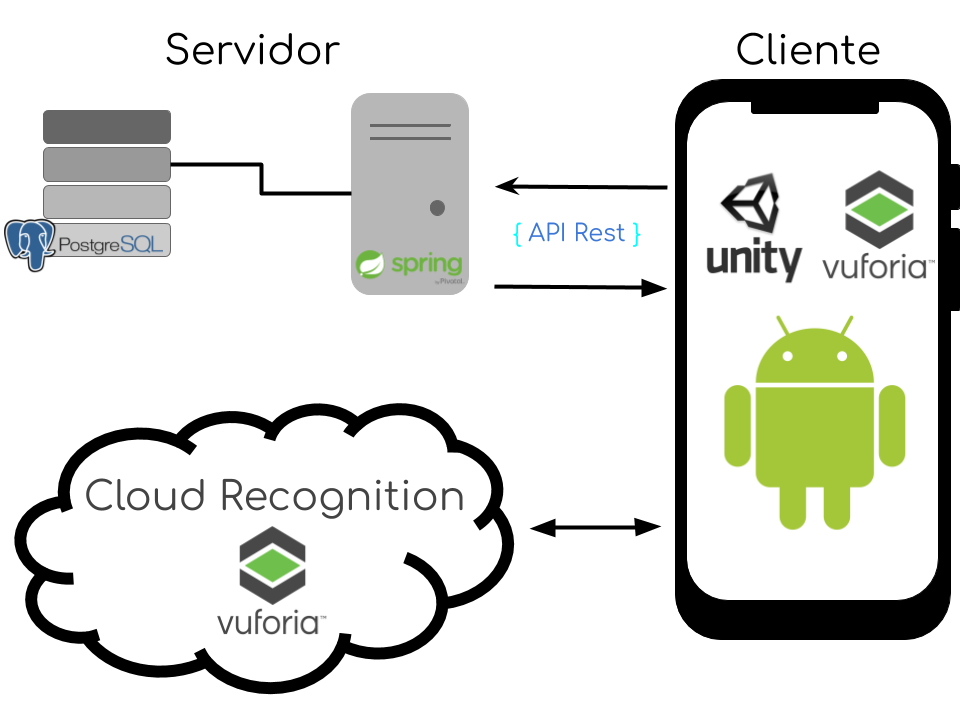
\includegraphics[width=6in]{figures/chapter-4/arquitectura.png}
    \caption{Arquitectura}
    \label{fig:arquitectura}
\end{figure}
\section{Servidor}
\label{makereference4.3}
Nuestro servidor está programado en Java, usando el framework Spring para la creación de una API Rest que, mediante peticiones HTTP y una base de datos relacional en PostgreSQL, nos proporcionará
toda la información necesaria para alimentar de datos a nuestro cliente. También se encuentra en el servidor la implementación del sistema de recomendación.
\subsection{Entidades}
\label{makereference4.3.1}
En el servidor tendremos todas las entidades que necesitamos
 (Ver \autoref{fig:modelo-ER}), estas son representadas
 mediante clases Java y anotaciones de JPA. Para facilitar el mapeo entre
 tablas de la base de datos y dichas entidades.
Hemos implementado las siguientes entidades:
\begin{figure}[H]
    \centering
    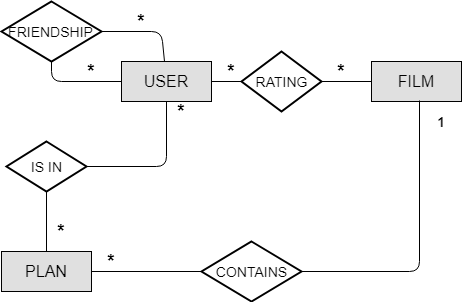
\includegraphics[width=6in]{figures/chapter-4/Entidades-ER.png}
    \caption{Modelo entidad-relación}
    \label{fig:modelo-ER}
\end{figure}
\begin{itemize}
    \item Film: entidad referente a las películas que guardamos, con su respectivo título, director, duración, valoración, url del tráiler, sinopsis, url de la imagen de la película, género, país y fecha de estreno.
    \item User: entidad para representar a los usuarios de la aplicación, con su nombre, foto, email y contraseña.
    \item Friendship: entidad para representar la relación de amistad entre usuarios.
    \item Plan: entidad para representar los planes. Estos poseerán una película, un usuario creador, fecha, hora, lugar, título, descripción y una lista de usuarios unidos.
    \item UserFilm: entidad intermedia para representar la relación de usuarios con películas, es decir, las películas que son guardadas por cierto usuario.
\end{itemize}
\subsection{Sistemas de recomendación}
\label{makereference4.3.2}
Implementamos el sistema de recomendación para obtener películas y planes
que pueden ser interesantes para cada usuario, en base a sus gustos.
Estas recomendaciones se utilizan en la parte de cliente y se muestran al
usuario a través de la interfaz.
La aplicación de Android se comunica con el servidor usando la
 API REST (Ver \autoref{makereference4.3.3}).
En la que disponemos de todas las búsquedas necesarias.
Los datos de las recomendaciones se guardan en una tabla de la base de datos.
Cada periodo de tiempo establecido previamente un procedimiento se ejecuta
 y actualiza la tabla para aplicar los nuevos datos guardados a las recomendaciones.
Este procedimiento usa una funcionalidad de la librería Mahout,
 para extraer los datos de valoraciones de usuarios a películas.
Con estos datos y usando una técnica de filtrado colaborativo genera las recomendaciones.
Como generar las recomendaciones es un proceso costoso y lento guardamos los
 resultados para ser utilizados.

\subsection{Controladores}
\label{makereference4.3.3}
Para cada una de estas entidades necesitamos una clase Controller, que actuará de controlador para saber redirigir cada petición HTTP a su correspondiente servicio de aplicación, donde se aplicará la lógica del negocio, comprobando 
que los datos son correctos y obteniendo, modificando o creando elementos en la base de datos a través de las clases Repository correspondiente a cada entidad.
A la búsqueda por ID tuvimos que añadir la búsqueda por UUID en usuarios y películas.
El ID es necesario para utilizarlo en el sistema de recomendación de Mahout y
el UUID es necesario para el reconocimiento de imágenes de Vuforia.
Las distintas peticiones HTTP que realizamos son las siguientes:

\begin{center}
    \begin{tabularx}{1\textwidth}{@{\extracolsep{\fill}} | l | l | X |} \hline
    \multicolumn{3}{|c|}{Film} \\ \hline
    Obtener todas las películas & GET & /films/ \\ \hline
    Guardar una película & POST & /films/ \\ \hline
    Actualizar una película & PUT & /films/ \\ \hline
    Buscar una película por su nombre & GET & /films/search/\{name\} \\ \hline
    Buscar una película por su id & GET & /films/\{id\} \\ \hline
    Buscar una película por su uuid & GET & /films/uuid/\{uuid\} \\ \hline
    Borrar una película & DELETE & /films/\{id\} \\ \hline
    \end{tabularx}
\end{center}

\begin{center}
    \begin{tabularx}{1\textwidth}{@{\extracolsep{\fill}} | l | l | X |} \hline
    \multicolumn{3}{|c|}{User} \\ \hline
    Obtener todos los usuarios & GET & /users/ \\ \hline
    Guardar un usuario & POST & /users/ \\ \hline
    Actualizar un usuario & PUT & /users/ \\ \hline
    Buscar un usuario por su nombre & GET & /users/search/\{name\} \\ \hline
    Buscar un usuario por su id & GET & /users/\{id\} \\ \hline
    Buscar un usuario por su uuid & GET & /users/uuid/\{uuid\} \\ \hline
    Borrar un usuario & DELETE & /users/\{id\} \\ \hline
    Obtener amistades de un usuario & GET & /users/\{id\}/friendships \\ \hline
    Obtener amigos de un usuario & GET & /users/\{id\}/friends \\ \hline
    Obtener planes de un usuario & GET & /users/\{id\}/plans \\ \hline
    Obtener películas que gustan a un usuario & GET & /users/\{id\}/films \\ \hline
    Login de un usuario & POST & /users/login \\ \hline
    \end{tabularx}
\end{center}

\begin{center}
    \begin{tabularx}{1\textwidth}{@{\extracolsep{\fill}} | l | l | X |} \hline
    \multicolumn{3}{|c|}{UserFilm} \\ \hline
    Obtener todas las valoraciones & GET & /user-films/ \\ \hline
    Guardar valoración & POST & /user-films/ \\ \hline
    Actualizar valoración & PUT & /user-films/\{userId\}/\{filmId\}/rate/\{rating\} \\ \hline
    Buscar una valoración & GET & /user-films/\{userId\}/\{filmId\} \\ \hline
    Borrar una valoración & GET & /user-films/\{id\} \\ \hline
    \end{tabularx}
\end{center}
\begin{center}
    \begin{tabularx}{1\textwidth}{@{\extracolsep{\fill}} | l | l | X |} \hline
    \multicolumn{3}{|c|}{Recommender} \\ \hline
    Obtener todas las recomendaciones & GET & /recommendations/ \\ \hline
    Obtener películas random & GET & /recommendations/random \\ \hline
    Obtener películas más relevantes & GET & /recommendations/trending \\ \hline
    Obtener películas más nuevas & GET & /recommendations/premiere \\ \hline
    Recomendaciones para un usuario & GET & /recommendations/\{id\} \\ \hline
    Obtener las recomendaciones de planes & GET & /recommendations/\{id\}/plans/\{friend\} \\ \hline
    Borrar todas las recomendaciones & DELETE & /recommendations/ \\ \hline
    Borrar todas las recomendaciones & DELETE & /recommendations/\{id\} \\ \hline
    \end{tabularx}
\end{center}
\begin{center}
    \begin{tabularx}{1\textwidth}{@{\extracolsep{\fill}} | l | l | X |} \hline
    \multicolumn{3}{|c|}{Images} \\ \hline
    Obtener imagen & GET & /\{image\}/ \\ \hline
    \end{tabularx}
\end{center}
\begin{center}
    \begin{tabularx}{1\textwidth}{@{\extracolsep{\fill}} | l | l | X |} \hline
    \multicolumn{3}{|c|}{Friendships} \\ \hline
    Obtener todas las amistades & GET & /friendships/ \\ \hline
    Petición de amistad & POST & /friendships/\{requesterId\}/\{friendId\}/request \\ \hline
    Aceptación de amistad & POST & /friendships/\{requesterId\}/\{friendId\}/accept \\ \hline
    Declinar amistad & DELETE & /friendships/\{requesterId\}/\{friendId\}/decline \\ \hline
    Eliminar amistad & DELETE & /friendships/\{requesterId\}/\{friendId\} \\ \hline
    \end{tabularx}
\end{center}
\begin{center}
    \begin{tabularx}{1\textwidth}{@{\extracolsep{\fill}} | l | l | X |} \hline
    \multicolumn{3}{|c|}{Plans} \\ \hline
    Obtener todos los planes & GET & /plans/ \\ \hline
    Guardar un plan & POST & /plans/ \\ \hline
    Unirse a un plan & PUT & /plans/\{id\}/join/\{userId\} \\ \hline
    Eliminar un plan & DELETE & /plans/\{id\} \\ \hline
    Obtener planes por id & GET & /plans/\{id\} \\ \hline
    Obtener los usuarios unidos a plan & GET & /plans/\{id\}/joined-users \\ \hline
    Obtener los usuarios de un plan & GET & /plans/\{id\}/users \\ \hline
    Buscar un plan por nombre & GET & /plans/search/\{title\} \\ \hline
    \end{tabularx}
\end{center}

\section{Cliente}
\label{makereference4.4}
Nuestra aplicación está implementada principalmente en Android, las interfaces principales para el uso de los planes, recomendaciones y acceso a la información de las películas guardadas han sido desarrolladas mediante Android Studio. Sin embargo,
la parte del cliente que otorga el gran valor a nuestra aplicación está desarrollada en Unity y el uso de Vuforia, todas las escenas que aparecen al reconocer carteles de películas e imágenes de usuarios fueron implementadas de esta forma.
La parte de la aplicación realizada en Unity, utiliza una serie de clases de la parte desarrollada en Android para realizar las peticiones al servidor y así poder mostrar información específica cuando se reconoce una cierta imagen.
Al principio la parte de Android implementaba la obtención de datos del servidor que necesitaba y la parte de Unity la suya. Después decidimos implementar la obtención de datos únicamente en Android y hacer usarlo desde Unity para tener mejor control y no duplicar soluciones al mismo problema.
Las imágenes que mostramos en la parte de Android se almacenan en el mismo servidor.


Como la mayor parte de la aplicación está implementada en Android Studio, la estructura de ésta se adapta a lo que ofrece el IDE, consistiendo en el flujo de unas actividades y fragmentos que explicaremos a continuación.


\subsection{Actividades}
\label{makereference4.4.1}
Son los componentes de la aplicación que representan una pantalla con la que
 los usuarios pueden interactuar para realizar una determinada
 acción (ver \autoref{fig:activity}).
\begin{figure}[H]
    \centering
    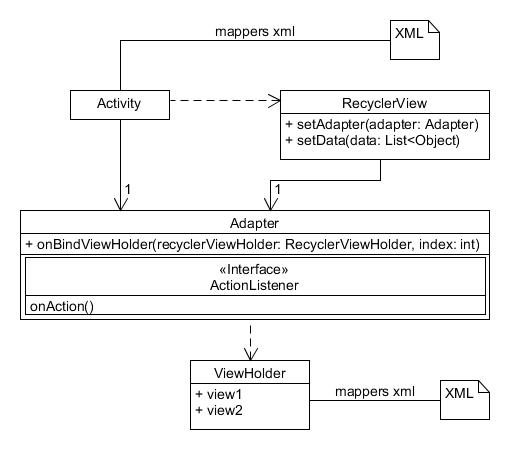
\includegraphics[width=6in]{figures/chapter-4/recyclerView.jpg}
    \caption{Actividades}
    \label{fig:activity}
\end{figure}

Entre nuestras actividades podemos destacar dos: 
\begin{itemize}
    \item MainActivity: La primera actividad (actividad principal) que se activa al iniciar la aplicación, la cual comprueba el estado de sesión del usuario, si está logueado se queda en la actividad, y si no, se redirige al usuario a otra actividad llamada LoginActivity que mediante un formulario muy simple nos permite iniciar sesión o registrarnos. En MainActivity se encuentra un paginador (ViewPager) de 3 fragmentos, donde cada fragmento representa las interfaces de planes, recomendaciones y películas guardadas correspondientemente. Podemos observarlo en la \autoref{fig:listaPlanes}, \autoref{fig:lista_peliculas} y \autoref{fig:recomendaciones_1} del \autoref{makereference3}.
    \item UnityPlayerActivity: Se trata de una actividad especial que nos permite comunicar la parte desarrollada en Unity con nuestro proyecto Android. Aquí se encuentran llamadas a funciones desde la parte de Unity, se realizan las órdenes y se devuelven a Unity.
\end{itemize} 

\subsection{Adaptadores}
\label{makereference4.4.2} 
Son elementos de manipulación de datos que se aplican a vistas y componentes. En el proyecto se les ha dado mucho uso a las vistas de tipo RecyclerView para representar listas de objetos. Para manejar los datos de cada elemento de la lista, se ha utilizado un RecyclerView.Adapter, el cual manipula cada dato correspondiente a un elemento de la lista. También se han creado otros adaptadores, como uno para manejar tres fragmentos dentro de una actividad, como hemos dicho anteriormente al describir la actividad principal (MainActivity).

\subsection{Comandos}
\label{makereference4.4.3}
Aquí se encuentran todos los elementos relacionados con el patrón comando (ver \autoref{fig:comando}).
Ha sido diseñado para realizar la conexión con la parte del proyecto desarrollado en Unity.
Al principio las peticiones al servidor se realizaban tanto en Android como en
Unity. Esto causaba que tuviéramos implementaciones duplicadas y originaba
 problemas si había que modificar estos métodos, porque era necesario aplicar los
 cambios en ambas capas.
Decidimos utilizar desde Unity los métodos de Android para resolver el problema.
Para evitar que Unity tuviera múltiples dependencias con la capa de Android,
 decidimos aplicar el patrón comando.
Este patrón nos permite abstraer la capa de Android con la capa de Unity y
 minimizar las dependencias que eran necesarias.

\begin{figure}[H]
    \centering
    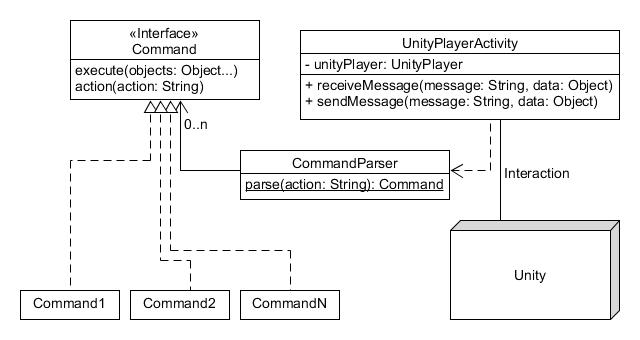
\includegraphics[width=6in]{figures/chapter-4/command.jpg}
    \caption{Patrón comando}
    \label{fig:comando}
\end{figure}



\subsection{Entidades}
\label{makereference4.4.4}
Todos los modelos de datos que podemos recibir del servidor, los cuales hemos descrito anteriormente en este capítulo, en la Sección 4.3, son representados por entidades en nuestro proyecto de Android, con los mismos atributos que tienen sus entidades correspondientes en el servidor.

\subsection{Fragmentos}
\label{makereference4.4.5}
Representan un comportamiento o una parte de la interfaz de usuario en una actividad.
Se utilizan para formar una vista compuesta de paginación en una actividad. 
Aquí es donde tendremos los 3 componentes principales de nuestra aplicación, la actividad referente a mis planes, la actividad de las recomendaciones y la de mis películas.

\subsection{Petición de servicios}
\label{makereference4.4.6}
Se trata de un conjunto de clases que solo poseen métodos estáticos para llevar
 a cabo peticiones HTTP al servidor. Se ha creado una clase genérica para la
 creación y llamada de peticiones HTTP, se ha diseñado de manera que las
 respuestas se devuelvan en forma de callback para un uso más sencillo
 (ver \autoref{fig:server}).
\begin{figure}[H]
    \centering
    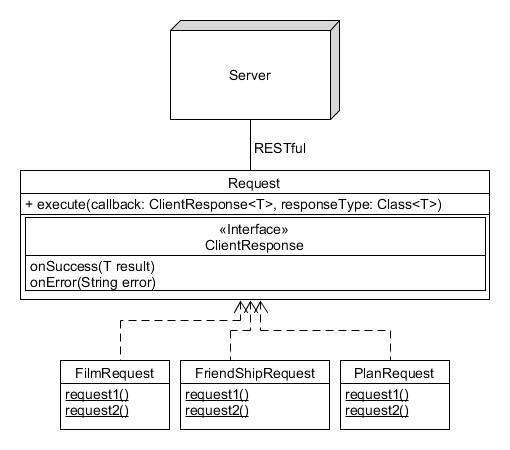
\includegraphics[width=6in]{figures/chapter-4/request.jpg}
    \caption{Petición de servicios}
    \label{fig:server}
\end{figure}
Los servicios que hemos implementado son los siguientes:
\begin{itemize}
    \item FilmRequest: servicio encargado de realizar las peticiones sobre películas al servidor, como podría ser buscar una película por su ID.
    \item FriendshipRequest: servicio responsable de obtener los datos relacionados a las relaciones entre amistad, como podría ser aceptar una petición o comprobar si dos usuarios son amigos.
    \item PlanRequest: servicio cuya finalidad es la de conseguir la información relacionada con los planes, como podría ser la operación de crear un plan y unirse o salirse de uno ya existente.
    \item RecommendationRequest: este servicio se ocupa de obtener las distintas recomendaciones de películas y planes de un usuario.
    \item UserFilmRequest: servicio creado para obtener la información referente a ciertos métodos de la relación entre películas y usuarios. Por ejemplo, con este servicio podríamos guardar una película como favorita de un usuario. También es usado para cuando un usuario valora cierta película.
    \item UserRequest: servicio que nos permite obtener todo lo relacionado con los usuarios, ya sean sus perfiles, los amigos de un usuario, los planes en los que está o las películas que ha guardado.
\end{itemize}

\subsection{Vistas}
\label{makereference4.4.7}
Entre los componentes que ofrece Android existen algunas funcionalidades no soportadas. Por ello hemos creado componentes personalizados para satisfacer estas funcionalidades:
\begin{itemize}
    \item AnchorVisibilityBehavior: Implementa el comportamiento de los elementos que aparecen y desaparecen en las actividades, por ejemplo, en la \autoref{fig:info_planes} tenemos un botón para la información de la película pero al hacer el scroll hacia abajo, en la \autoref{fig:info_planes_1}, vemos que éste desaparece.
    \item CustomViewPager: el ViewPager es lo que usamos en la MainActivity para colocar los tres fragmentos. Se crea esta clase para desactivar la acción de cambiar entre fragmentos al deslizar con el dedo en la pantalla del smartphone. Esto nos daba problemas debido a que en el fragmento de las recomendaciones tenemos elementos con scroll horizontal y la acción de deslizar con el dedo en la pantalla interfería.
    \item ExpandableTextView: Es una clase que extiende de un TextView, se le añade un método para que cuando haya mucho texto, se pueda acortar. Además dispone de un botón para expandir.
\end{itemize} 

\section{Despliegue}
\label{makereference4.6}
El servidor puede desplegarse como un Docker o en Heroku.
Para el desarrollo del proyecto hemos utilizado Heroku por la facilidad y
comodidad que ofrece. 
Usamos una cuenta gratuita que nos permite un alojamiento limitado con las
 características suficientes para el desarrollo del proyecto.
Utilizamos un despliegue automático que al realizar cambios en una rama del
 repositorio de GitHub, Heroku descarga esos cambios y lo despliega en el servidor.
En la \autoref{app:heroku} encontramos una guía de como desplegar la
aplicación con tu usuario de Heroku. En la \autoref{app:docker} vemos como
desplegar la aplicación en un Docker.

\section{Herramientas de trabajo}
\label{makereference4.7}
Las distintas herramientas de trabajo que hemos decidido usar para que el trabajo realizado fuera más eficiente son las siguientes:
\begin{itemize}
    \item Telegram: hemos usado esta aplicación de mensajería para poder comunicarnos entre todos los miembros pertenecientes al proyecto, ya fuera para la sugerencia de ideas o que un bot de GitHub nos avisara de los cambios en los distintos repositorios que hemos creado. 
    \item Slack: esta otra herramienta de comunicación nos ha permitido crear canales específicos para cada parte de nuestro proyecto y así poder clasificar las conversaciones que teníamos por temas, por ejemplo, tenemos un canal para hablar solo de la parte backend, otro para hablar de la parte de realidad aumentada, etc. Cosa que Telegram no nos permitía y resultaba lioso encontrar ciertos temas o puntos de nuestras conversaciones. 
    \item Trello: nos ha servido como apoyo para realizar nuestros sprints, Trello nos ofrece la posibilidad de crear un tablero para escribir tareas a modo de post-it y asignarlas a usuarios que estén dentro del tablero, así sabemos qué tipo de tareas ha realizado o está realizando cada miembro en todo momento.
    \item GitHub: todos nuestros repositorios están en GitHub, lo que nos permite subir cambios y trabajar en paralelo en distintas ramas, agilizando así nuestro trabajo y otorgándonos un control de versiones muy estable.
    \item Visual Studio Code: utilizamos este editor de código junto con la extensión de LaTeX Workshop para escribir la memoria en LaTeX.
    \item Android Studio: usamos este IDE para construir la aplicación Android que además nos dota de herramientas de depuración.
    \item Google Drive: almacenamiento en la nube donde tenemos toda la información relevante para el TFG.
    \item Heroku: plataforma en la que desplegamos nuestra aplicación de servidor.
    \item Unity: Utilizamos esta plataforma de desarrollo para construir la parte de la aplicación relacionada con Realidad Aumentada.
    \item Visual Studio: Utilizamos Visual Studio para codificar los scripts en C\# necesarios para el funcionamiento de la parte de realidad aumentada en Unity.
    \item Postman: aplicación para el envío de peticiones HTTP REST, que utilizamos para depurar los servicios de Spring.
    \item MockFlow: herramienta online para el diseño de mockups, nosotros la utilizamos para el diseño de las vistas de la aplicación Android.
\end{itemize}

\section{Conclusiones}
\label{makereference4.8}
A continuación, mostraremos una lista de todas las dificultades encontradas a la hora de implementar nuestra aplicación:
\begin{itemize}
    \item Diseño de las interfaces para que fueran familiares e intuitivas para el usuario. Tuvimos que rehacer muchas veces los distintos bocetos de las interfaces ya que no eran intuitivos para los usuarios. Gracias a las sugerencias que se nos iban haciendo conseguimos mejorarlas bastante.
    \item Desconocimiento del entorno de desarrollo y peculiaridades del desarrollo de aplicaciones en Android. Para resolver nuestro desconocimiento de Android realizamos una serie de prototipos y buscamos tutoriales que nos sirvieran como ejemplo para desarrollar cada parte de nuestra aplicación.
    \item Incompatibilidad de realización de peticiones HTTP en ciertas versiones de Android. Tras probar la aplicación en un smartphone con versión de Android 9.0 descubrimos que los permisos para hacer peticiones de este tipo a un servidor no funcionaban con la configuración inicial de nuestro proyecto. Para solucionarlo cambiamos una serie de líneas de código en nuestro archivo AndroidManifest.xml para solventarlo.
    \item Problemas a la hora de intentar desplegar el servidor de forma correcta para que fuera accesible siempre. Para que el servidor estuviera siempre levantado se nos ocurrió realizar su despliegue en Heroku para así poder realizar peticiones en cualquier momento desde la app.
    \item Poca familiaridad con el uso de Unity y el lenguaje C\# para realizar la parte de realidad aumentada. Para familiarizarnos con el entorno implementamos una serie de prototipos y buscamos tutoriales que nos sirvieran como guía para diseñar nuestra parte de realidad aumentada. 
    \item Caducidad de las licencias gratuitas para el uso del Cloud de Vuforia. La solución a este problema fue muy simple, crearnos cuentas nuevas cada vez que se acabara la licencia para poder seguir accediendo a este servicio.
    \item Primera vez usando el framework de Spring para la realización de una API Rest. Su solución fue seguir un tutorial paso a paso para crearlo con una sola entidad e ir ampliándolo a todas las entidades que necesitaba nuestra aplicación.
    \item Comunicación entre la parte cliente en Android y el servidor. Conseguimos realizar servicios en Android que realizaban las peticiones al servidor de forma asíncrona, obteniendo su resultado en una función callback para usar dicha información como correspondiera en cada caso.
    \item Comunicación entre la parte cliente en Unity con la parte cliente en Android. Para abstraer la lógica desarrollada en Android a la de Unity implementamos clases que usaban el patrón Command para facilitar la comunicación entre estas dos partes de nuestro proyecto.
    \item Rendimiento en cuanto al reconocimiento de ciertas imágenes, sobre todo de personas, debido a la calidad de las mismas. El Cloud de Vuforia no las reconoce tan fácilmente como las de carteles de películas. Para arreglarlo tuvimos que buscar imágenes de usuarios con una mejor calidad para facilitar a la librería su reconocimiento, finalmente optamos por poner imágenes de los integrantes del proyecto durante el desarrollo de la aplicación.
    \item Almacenamiento de imágenes en Google Drive y su obtención desde Android y Unity, junto con el retardo que esto produce. Para no tener las imágenes de los usuarios en la aplicación se nos ocurrió guardarlas en Google Drive y obtenerlas con la librería de Picasso de Android, pero esto era muy lento y decidimos guardarlas en el mismo servidor.
    \item Incompatibilidades con las nuevas actualizaciones de Unity. Hemos tenido cuidado con no actualizar el IDE de Unity porque nuestro proyecto quedaría obsoleto, ya nos vimos en la situación de que uno de los miembros tenía una versión superior a la de los demás y tuvimos que rehacer lo que habíamos implementado.
\end{itemize}
% +--------------------------------------------------------------------+
% | Sample Chapter 5
% +--------------------------------------------------------------------+

\cleardoublepage

% +--------------------------------------------------------------------+
% | Replace "This is Chapter 5" below with the title of your chapter.
% | LaTeX will automatically number the chapters.
% +--------------------------------------------------------------------+

\chapter{Conclusiones}
\label{makereference5}
Cuando comenzamos a hablar sobre este proyecto, lo que nos motivó fue el
 reto de aprender nuevas tecnologías desconocidas para nosotros y afrontarlas
 en un proyecto que soluciona un problema concreto. La solución a este problema
 es una aplicación móvil que nos ofrece la facilidad de crear y gestionar
 planes con amigos para ir al cine. Usando un sistema de recomendación somos
 capaces de tener una previsión sobre lo que nos podría gustar la película en
 base a otras que hayamos valorado anteriormente.
 Con el uso de tecnología de RA buscamos que el usuario se sienta más cómodo
 utilizando la aplicación sin tener que introducir muchos datos, si no que el propio
 dispositivo móvil sea capaz de reconocer los carteles de películas o imágenes
 de usuarios y nos ofrezca acciones sobre ello.

Al principio buscamos aprender los aspectos más básicos que nos permitieran
 diseñar e implementar de la aplicación. Para ello realizamos un estudio
 del estado del arte en el que desempeñamos las siguientes tareas:
\begin{itemize}  
    \item Buscamos información y explicamos que es la realidad aumentada y cuál es su
        estado actual. Describimos diferentes librerías de realidad aumentada con sus
        aspectos más destacables.
    \item Descubrimos y especificamos distintas fuentes de información de las cuales extraer
        los datos necesarios sobre las películas de la aplicación que se mostrara o se utilizaran
        para el sistema de recomendación.
    \item Buscamos información sobre los distintos tipos de técnicas de recomendación y
        definimos las más interesantes.
\end{itemize}


En el siguiente paso, diseñamos la aplicación y definimos su funcionalidad,
 realizando las siguientes tareas:
\begin{itemize}
    \item Realizamos un análisis de competencia en el cual descubrimos aplicaciones
        similares que nos ayudaron a visualizar el diseño de nuestra aplicación.
    \item Definimos escenarios donde se podría usar nuestra aplicación.
    \item En base a los escenarios anteriormente definidos, establecimos los requisitos
        funcionales que describen la funcionalidad de la aplicación.
    \item Diseñamos las interfaces de la aplicación para las funcionalidades anteriormente
        comentadas.
\end{itemize}

Posteriormente, pasamos a la parte de implementación donde realizamos las siguientes
 tareas:
\begin{itemize}
    \item Desarrollamos prototipos con distintas librerías de realidad
        aumentada en aplicaciones móviles y valoramos la experiencia con ellas.
    \item Definimos una arquitectura REST para nuestra aplicación y un reconocimiento
        de imágenes en la nube.
    \item Implementamos un servidor en Spring desplegado en Heroku
        que usa como base de datos PostgreSQL.
    \item Implementamos la aplicación móvil en Android, la parte de RA en Unity con la
        librería Vuforia.
    \item Valoramos distintos sistemas de recomendación y finalmente lo implementamos
        con Mahout.
\end{itemize}

Finalmente, fuimos capaces de aplicar los conceptos generales que aprendimos
 en el grado en un entorno nuevo y desafiante, gracias al valor humano de
 un equipo multidisciplinar en el cual los integrantes complementan sus
 puntos débiles individuales. 

% +--------------------------------------------------------------------+
% | Sample Chapter 6
% +--------------------------------------------------------------------+

\cleardoublepage

% +--------------------------------------------------------------------+
% | Replace "This is Chapter 6" below with the title of your chapter.
% | LaTeX will automatically number the chapters.
% +--------------------------------------------------------------------+

\chapter{Trabajo futuro}
\label{makereference6}
Uno de los mayores problemas del proyecto fue la dificultad de integrar
 distintas tecnologías entre sí y que estas cumplieran con todos los requisitos
 que buscábamos. Esto ocasiono que el tiempo de aprendizaje y adaptación del uso
 de estas tecnologías se disparará, por tanto, a las primeras funcionalidades que
 teníamos en mente tuvimos que priorizar las que daban el uso básico al problema
 que planteábamos.
A continuación, destacaremos todas esas funcionalidades o mejoras que nos
 gustaría que tuviera en un futuro la aplicación para que la usabilidad y
 posibilidades sean más ricas para el usuario:
\begin{enumerate}
    \item Una de las situaciones que se pueden encontrar nuestros usuarios es
     que quieren ir al cine a ver una película con amigos, pero no les importe
     que película si no pasar un buen rato con buena compañía. En este caso la
     aplicación podría crear planes y una vez se unan todos los amigos sea capaz
     de recomendar la película que mejor se ajusta a sus preferencias.
    \item Otra situación similar a la anterior es que queramos que nos
     recomiende la película que mejor se adapta a los gustos del grupo, pero
     acotando a las películas que elijamos previamente.
    \item En el momento del desarrollo de este proyecto el reconocimiento facial
     no está integrado en las librerías de RA que hemos investigado y la
     complejidad de integrar tecnologías de reconocimiento facial, así como su
     aprendizaje no era viable para el tiempo de este proyecto.
    Con lo que se decidió realizar el reconocimiento del usuario con imágenes
     asemejando esta funcionalidad. Creemos interesante el uso de
     reconocimiento facial para funcionalidades de usuario, aunque pueda ser
     polémica es algo nuevo que aporta valor a la aplicación.
    \item La escena de RA esta implementada en Unity por lo que podemos
     exportarla a otras plataformas como iOS, consiguiendo con esto que la
     aplicación se abra a más usuarios y estos consigan un mayor crecimiento y
     enriquecimiento de la aplicación.
    \item Facilitar la compra de entradas desde la aplicación para que los
     usuarios puedan realizar la mayoría de las acciones, necesarias para ir al
     cine, redireccionando a la página web de venta de los cines a los que se
     quieren acudir para ver la película.
    \item Publicar la aplicación a una plataforma de distribución digital de
    aplicaciones como Google Play, para que los usuarios tengan acceso a
    instalarla en sus dispositivos.
    \item Automatizar con web scraping la obtención de datos de las fuentes de
     información de películas para que la aplicación siempre tenga la
     información actual.
    \item Utilizar distintos idiomas para el contenido de las películas en la
     base de datos del servidor usando una columna que indique el idioma de la
     información.
    \item Una de las cosas más importantes que falta por realizar es una
     evaluación con usuarios que nos proporcionen retroalimentación de la
     aplicación de la cual obtendremos una visión más amplia sobre si satisface
     la necesidad al problema que tratamos en el proyecto o si hay que realizar
     cambios. 
\end{enumerate}
% +--------------------------------------------------------------------+
% | Sample Chapter 7
% +--------------------------------------------------------------------+

\cleardoublepage

% +--------------------------------------------------------------------+
% | Replace "This is Chapter 7" below with the title of your chapter.
% | LaTeX will automatically number the chapters.
% +--------------------------------------------------------------------+

\chapter{Contribución al proyecto}
\label{makereference7}
En este capítulo especificaremos las aportaciones de cada integrante del grupo,
 las cuales se ordenarán por las fases del proyecto.

\section{Diego Acuña Berger}
\label{makereference7.1}
    \subsection{Estado del arte}
    \label{makereference7.1.1}
        \begin{itemize}
            \item Investigación de las distintas fuentes de información para la obtención de los datos referentes para las películas, valorando cuál sería la que mejor información aportaba para el proyecto.
        \end{itemize}
    \subsection{Diseño de la aplicación}
    \label{makereference7.1.2}
        \begin{itemize}
            \item Diseños de vistas de la aplicación con MockFlow. Es decir, el diseño de los primeros bocetos de las interfaces que terminaron por ser lo que hemos diseñado en el capítulo 3.
            \item Diseño de las interfaces de usuario de los planes y películas
            guardadas. Tras varias pruebas y diseños fallidos diseñé la forma de mostrar los planes y películas basándome en aplicaciones del ámbito del cine o de las series, como puede ser TV Time \cite{tvtime}
            \item Diseño de la vista que aparece tras guardar una película mediante la realidad aumentada, con la que se confirma que película se ha guardado.
        \end{itemize}
    \subsection{Implementación}
    \label{makereference7.1.3}
        \begin{itemize}
            \item Estudio y creación del prototipo de servidor en Spring. Búsqueda de tutoriales y la codificación de un pequeño servidor en local usando el framework de Spring, tras el prototipo contribuí a su ampliación y modificación para que se ajustase correctamente a lo que necesitaba nuestra aplicación.
            \item Obtención de imágenes mediante Picasso a la aplicación. 
            \item Funcionalidad para guardar películas mediante realidad aumentada, esto implica la comunicación con Android y Unity para saber la relación que tiene la película que se ha reconocido desde el cloud, con la película que se guarda en el servidor y otorgar feedback al usuario de su correcto funcionamiento.
            \item Disposición y diseño de botones que aparecen tras reconocer una
            película con realidad aumentada. Los botones que mostrábamos al principio no tenían mucho sentido con sus iconos y ocupaban mucho espacio, opté por incluir un botón inicial que al pulsarse se desplegase y mostrase más botones por encima del mismo, en los cuales puedes acceder a la información de la película o guardarla.
            \item Implementación de funciones del servidor tales como unirse a un plan, salirse de un plan y buscar los planes de un usuario concreto. Cuando me dedicaba a implementar ciertas vistas de la aplicación de Android, como mostrar los planes o las películas guardadas, me vi en la necesidad de incluir funciones en el servidor para obtener los datos que necesitaba, las cuales no nos habíamos planteado ninguno hasta el momento en el que fueron necesarias. 
        \end{itemize}
    \subsection{Memoria}
    \label{makereference7.1.3}
        \begin{itemize}
            \item Redacción del resumen tanto en español como en inglés.
            \item Redacción de la introducción a nuestro proyecto así como de los antecedentes.
            \item Redacción de las distintas interfaces de usuario de la aplicación.
            \item Redacción del prototipo del servidor que implementé con Spring.
            \item Redacción de cómo está implementado nuestro servidor, es decir, qué entidades poseemos, que servicios de aplicación, controladores y repositorios.
            \item Revisión de calidad de la memoria. Me he ocupado de revisar las posibles faltas ortográficas o fallos de estilo al usar LaTeX.
            \item Redacción de las dificultades de trabajo así como de las soluciones que les dimos durante el desarrollo del proyecto.
        \end{itemize}

\section{Daniel Calle Sánchez}
\label{makereference7.2}
    \subsection{Estado del arte}
    \label{makereference7.2.1}
        \begin{itemize}
            \item Estudio de la tecnologías de Realidad Aumentada, Viro React y
            Expo AR.
        \end{itemize}
    \subsection{Diseño de la aplicación}
    \label{makereference7.2.2}
        \begin{itemize}
            \item Identificación de requisitos funcionales de la aplicación.
            \item Diseños de vistas de la aplicación con MockFlow.
        \end{itemize}
    \subsection{Implementación}
    \label{makereference7.2.3}
        \begin{itemize}
            \item Creación de prototipo con ViroReact y ARCore.
            \item Diseño de la arquitectura.
            \item Configuración de Heroku.
            \item Implementación de servicios en Spring.
            \item Reconocimiento de usuarios con Vuforia en Unity.
            \item Desarrollo de vistas para planes en Android.
            \item Búsqueda y configuración de herramientas que mejoren el
             rendimiento del equipo.
        \end{itemize}
    \subsection{Memoria}
    \label{makereference7.2.3}
        \begin{itemize}
            \item Redacción de capítulo 5 Conclusiones.
            \item Redacción de capítulo 6 Trabajo futuro.
        \end{itemize}

\section{Carlos Gómez Cereceda}
\label{makereference7.3}
    \subsection{Estado del arte}
    \label{makereference7.3.1}
        \begin{itemize}
            \item
        \end{itemize}
    \subsection{Diseño de la aplicación}
    \label{makereference7.3.2}
        \begin{itemize}
            \item
        \end{itemize}
    \subsection{Implementación}
    \label{makereference7.3.3}
        \begin{itemize}  
            \item Creación de prototipo con ARCore en Android.
            \item Creación de prototipo con Vuforia en Unity.
            \item Creación de prototipo con Vuforia en Unity exportado a
             Android.
            \item Configuración del proyecto para poder tener la parte de
             Vuforia separada de la de Android.
            \item Comunicación entre la parte de Vuforia en Unity y la de
             Android.
            \item Configuración del proyecto para que se pueda comunicar con el
             Cloud de Vuforia.
            \item Creación de las primeras vistas prototipo del proyecto, tales
             como: Mostrar vídeos en \textbf{Realidad Aumentada}, botones y
             películas.
            \item Comunicación en Vuforia con el servidor.
            \item Creación de la vista en Unity que se muestra al identificar
             una película mediante \textbf{Realidad Aumentada}, además de su
             funcionalidad y comunicación con \textbf{Android}. Ejemplo: mostrar
             tráiler, puntuación, información…
            \item Creación de la vista en Unity que se muestra al identificar a
             un usuario no identificado como amigo. Así como la funcionalidad en
             Realidad Aumentada y Android para agregar a dicho usuario como
             amigo.
            \item Creación de la vista en Unity que se muestra al identificar a
             un amigo en donde se muestran los tres planes recomendados y la
             información visual de cuánto se prevé que les guste ese plan a los
             usuarios dentro del plan.
            \item Creación en Android de métodos de comunicación con el servidor
             para acciones como añadir amigos, borrar plan, añadir amigo,
             obtener amistad…
            \item Creación en el servidor de la primera versión de usuarios y su
             relación con películas.
        \end{itemize}
    \subsection{Memoria}
    \label{makereference7.3.3}
        \begin{itemize}
            \item
        \end{itemize}

\section{Zihao Hong}
\label{makereference7.4}
    \subsection{Estado del arte}
    \label{makereference7.4.1}
        \begin{itemize}
            \item Estudio de Vuforia + Android, de las dependencias que necesitaba. Investigación del pipeline 
            que usan para renderizar objetos en el espacio, la librería de dibujo en 3D que se usa internamente \textbf{OpenGL}, 
            incluso aprendizaje de lenguajes de bajo nivel (\textbf{GLSL}) que se usa en las tarjetas gráficas.
            \item Aprendizaje de los distintos métodos de recomendación, prueba, evaluación y final elección del algoritmo usado en el proyecto.  
        \end{itemize}
    \subsection{Diseño de la aplicación}
    \label{makereference7.4.2}
        \begin{itemize}
            \item Participación en escenarios diseñando algunos casos de escenarios como boceto.
            \item Diseño de las interfaces de usuario de los amigos y de sesión. Éstas interfaces se fueron cambiando con la implementación.
        \end{itemize}
    \subsection{Implementación}
    \label{makereference7.4.3}
        \begin{itemize}  
            \item Creadas cuentas para el cloud de vuforia y pruebas insertando imágenes y comprobación con prototipos.
            \item Creación de prototipo con Vuforia en Android, encontrándose con la dificultad de que se necesita programar con lenguajes a bajo nivel, entre otras cosas.
            \item Creación de prototipo de la arquitectura de Microservicios, para posterior incorporación en el proyecto.
            \item Creación, prueba, y evaluación de varios ejemplos de Unity con Realidad Aumentada y elección final para establecer el proyecto de Unity.
            \item Evaluación del uso del Docker ofrecido por la universidad, creación de scripts para imágenes de docker, como para el despliegue de proyectos de maven en un entorno Linux como un servicio. 
            \item Creación de la base de la de arquitectura del proyecto de Android y de las vistas que lo componen.
            \item Configuración del proyecto del servidor mediante maven y perfiles para el despliegue en un entorno Linux.
            \item Implementación de rutas en el servidor, como sus servicios de aplicación, repositorios, etc.
            \item Implementación en el servidor el sistema de recomendación por medio de la librería de mahout, que ofrece un método para la conexión con la base de datos \textbf{Postgresql} sin tener que leerlo de un fichero csv.
            \item Revisor de código.
            \item Establecimiento del uso de patrones de diseño, como comandos, singleton, constructor, etc. Los cuales se encuentran en la implementación de Android. 
        \end{itemize}
    \subsection{Memoria}
    \label{makereference7.4.3}
        \begin{itemize}
            \item
        \end{itemize}


% +-------------------------------------------------------------------------+
% | References                                                              |
% +-------------------------------------------------------------------------+

% +-------------------------------------------------------------------------+
% | In order for WinEDT to index references correctly, it has to know where |
% | the file resides.  The following command is prefaced by %, and will be  |
% | ignored completely by LaTeX.  However, WinEDT will use this line to     |
% | access the external .bib bibliography file.  Also note that WinEDT can  |
% | read file path names with either "\" or "/" - LaTeX, however, doesn't   |
% | like "\", so it's easier to store a path name in the "Unix" style.      |
% +-------------------------------------------------------------------------+

%Included for Gather Purpose only.  Do NOT uncomment:
%input "references.bib"

% +--------------------------------------------------------------------+
% | This template uses the BibTeX program to format references.  The
% | 3 lines below create a separate Bibliography section and add
% | an entry for "Bibliography" to the Table of Contents.  The actual
% | data for your references (author, title, journal, date, etc.) are
% | entered in the references.bib file.  See that file for information
% | on how to enter references.
% +--------------------------------------------------------------------+

\bibdata{references}
\bibliography{references}
\addcontentsline{toc}{chapter}{Bibliography}

% +--------------------------------------------------------------------+
% | Finally, we generate the appendix.  To add or delete appendices,
% | add or remove the line
% |
% |     \input{appendixX.tex}
% |
% | where "X" is the letter designation of the Appendix (A, B, C, etc.)
% | You should have one \input{appendixX.tex} line and a corresponding
% | file appendixX.tex for each appendix.                                 |
% +--------------------------------------------------------------------+

\appendix
% +--------------------------------------------------------------------+
% | Appendix A Page (Optional)                                         |
% +--------------------------------------------------------------------+

\cleardoublepage

\chapter{Guía de instalación para el servidor}
\label{app:guia_instalacion}

\section{Docker}
\label{app:docker}
Esta es una guía para el despliegue del servidor en Docker.

Para ello primero tenemos que tener una instancia de docker, si se quiere ejecutar en local, 
hay que instalar docker por el enlace \url{https://www.docker.com/}
La imagen de docker se descarga por git por el siguiente enlace:
\url{https://github.com/ZReKoJ/Docker.git}

\begin{lstlisting}[language=bash, caption=Dockerfile]
    FROM ubuntu:16.04

    RUN apt-get update 
    RUN apt-get install -y openssh-server
    RUN mkdir /var/run/sshd
    RUN echo 'root:tfg-ucm' | chpasswd
    RUN sed -i 's/PermitRootLogin prohibit-password/PermitRootLogin
         yes/' /etc/ssh/sshd_config
    
    # SSH login fix. Otherwise user is kicked off after login
    RUN sed 's@session\s*required\s*pam_loginuid.so@session optional
         pam_loginuid.so@g' -i /etc/pam.d/sshd
    
    ENV NOTVISIBLE "in users profile"
    RUN echo "export VISIBLE=now" >> /etc/profile
    
    EXPOSE 22 8000 8080
    CMD ["/usr/sbin/sshd", "-D"]
\end{lstlisting}

\begin{lstlisting}[language=bash, caption=Descarga de la imagen de docker]
    # Descarga de la imagen
    git clone https://github.com/ZReKoJ/Docker.git 
    # Entrar en la carpeta
    cd Docker 
    # Crear la imagen
    docker build --tag=filmar . 
\end{lstlisting}

\begin{figure}[H]
    \centering
    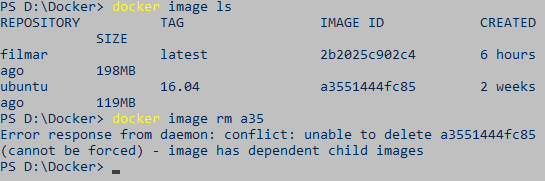
\includegraphics[width=6in]{figures/appendix-A/list-docker-images.png}
    \caption{Imágenes creadas de docker}
\end{figure}

Se han creado dos imágenes tras la ejecución, la de ubuntu es una dependencia usada, para tener el entorno de Linux, por eso no se puede borrar.

\begin{lstlisting}[language=bash, caption=Levantamiento de la instancia de docker]
    # Levanta docker mapeando puertos
    # Tras la ejecutar se va a quedar corriendo
    # Pulse Ctrl + C para parar
    # Pero estaria levantado el contenedor
    docker run -p 22022:22 -p 8080:8080 filmar 
    # No hace falta ejecutar los siguientes comandos
    # Comando para listar containers de docker corriendo
    docker ps 
    # Listar todos los containers
    docker container ls --all 
    # Parar el container
    docker stop 018 
    # Borrar el container
    docker rm 018 
\end{lstlisting}

\begin{figure}[H]
    \centering
    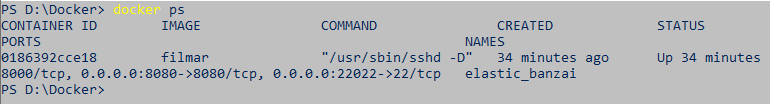
\includegraphics[width=6in]{figures/appendix-A/list-docker-containers.png}
    \caption{La instancia de docker levantada}
\end{figure}

Ahora que se ha levantado la instancia de docker con un ID 0186392cce18 y sus respectivos puertos mapeados.
Se conecta al container mediante ssh con la contraseña \textbf{tfg-ucm}

\begin{lstlisting}[language=bash, caption=Conexión ssh]
    # El puerto 22022 es el que se habia mapeado
    ssh root@localhost -p 22022
\end{lstlisting}

Una vez conectado al container, hay que instalar las siguientes herramientas

\begin{lstlisting}[language=bash, caption=Instalaciones]
    # Actualizacion por si acaso
    apt update 
    # Para descargar el repositorio en github
    apt install git
    # El servidor es un proyecto maven
    apt install maven
    # Base de datos
    apt install postgresql
    # Para usuarios
    apt install sudo
    # El servidor es un proyecto de java
    apt install openjdk-8-jdk
\end{lstlisting}

Una vez instalado todas las herramientas, descargar el proyecto del servidor,
que está en \url{https://github.com/DanielCalle/TFG-Server.git}

\begin{lstlisting}[language=bash, caption=Descarga del proyecto]
    # Se recomienda descargar el proyecto en la carpeta home
    cd /home
    git clone https://github.com/DanielCalle/TFG-Server.git
\end{lstlisting}

Antes de levantar el servicio, hay que preparar postgresql. El archivo SQL está dentro del proyecto
en el siguiente path: \url{/src/main/webapp/WEB-INF/sql/filmar_low.sql}

\begin{lstlisting}[language=bash, caption=Configuración postgresql]
    # Levantar postgresql
    service postgresql start
    # Cambiar al usuario postgres (por defecto)
    sudo -i -u postgres
    # Iniciar psql
    psql
    # Cambiar el password a 'admin'
    \password
    # Creacion de una base de datos
    create database films;
    # Salir de psql
    \q
    # Crear la estructura de base de datos
    # Anadir datos
    psql -d films -f /home/TFG-Server/src/main/webapp/
        WEB-INF/sql/filmar_low.sql
    # Salir del usuario postgres
    exit
\end{lstlisting}

Una vez configurado postgres, se procede al despliegue del servicio.

\begin{lstlisting}[language=bash, caption=Despliegue]
    # Acceder a la raiz del repositorio
    cd /home/TFG-Server
    # Empaquetar con el perfil de docker
    mvn package -P Docker
    # Dar permiso de ejecucion al script
    chmod +x server.sh
    # Ejecutar 
    ./server.sh start
    # No hace falta ejecutar los siguientes comandos
    # Para parar el servicio
    ./server.sh start
    # Para reiniciar el servicio
    ./server.sh restart
\end{lstlisting}

Ya está levantado el servicio en el puerto 8080, se puede probar con el siguiente enlace
\url{localhost:8080/films}.

\section{Heroku}
\label{app:heroku}
Para comenzar debemos crear una cuenta en \href{https://www.heroku.com/}{Heroku}.
Una vez la tenemos creamos una nueva aplicación a la
 cual daremos un nombre como vemos en la \autoref{fig:heroku_1} y este
 nombre a su vez será parte de la URL pública.
\begin{figure}[H]
    \centering
    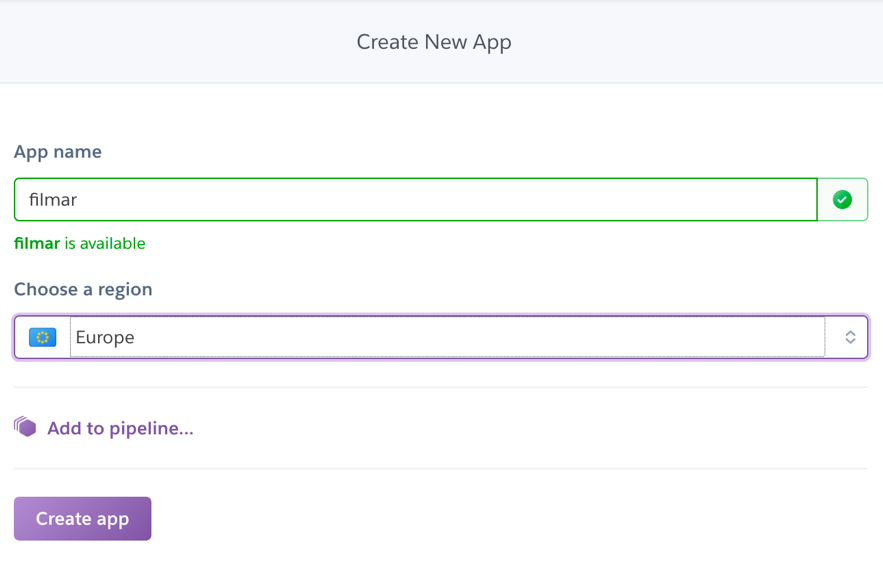
\includegraphics[width=6in]{figures/appendix-A/heroku_1.png}
    \caption{Crear nueva aplicación en Heroku}
    \label{fig:heroku_1}
\end{figure}
Cuando creemos la aplicación accederemos a la configuración en la que veremos
 opciones como en la figura \autoref{fig:heroku_2}.
\begin{figure}[H]
    \centering
    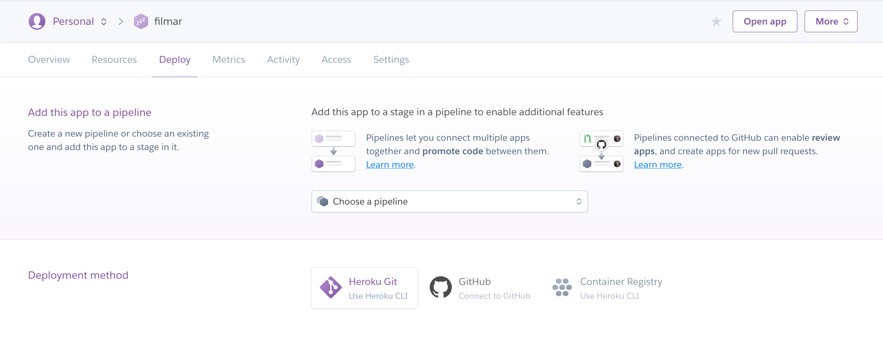
\includegraphics[width=6in]{figures/appendix-A/heroku_2.png}
    \caption{Configuración de la aplicación}
    \label{fig:heroku_2}
\end{figure}
Entramos en la pestaña de recursos y buscamos Postgres como vemos en la
\autoref{fig:heroku_3}. La seleccionamos y agregamos la versión gratuita.
\begin{figure}[H]
    \centering
    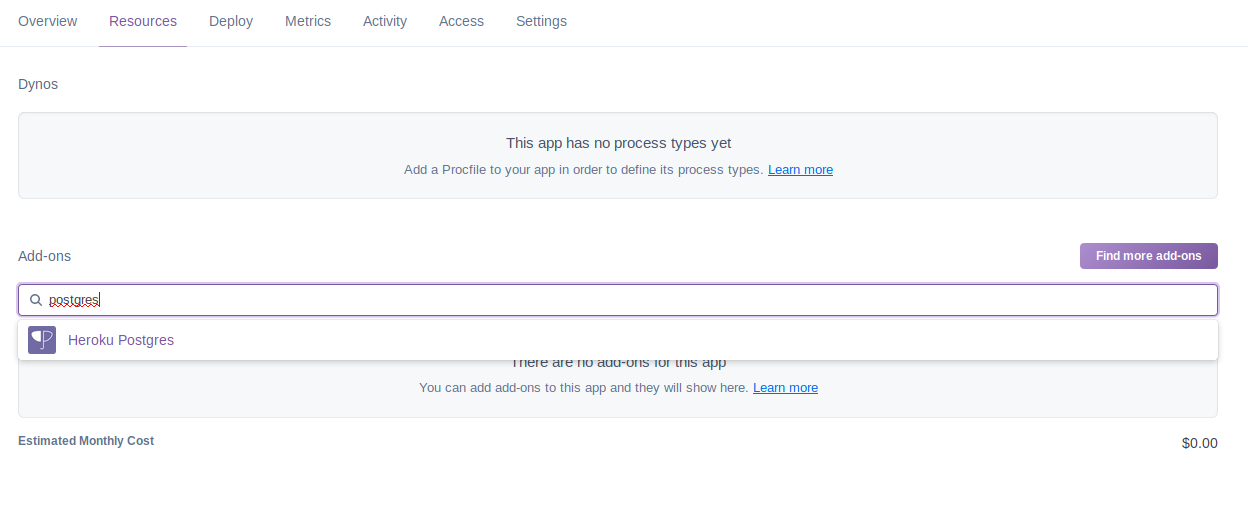
\includegraphics[width=6in]{figures/appendix-A/heroku_3.png}
    \caption{Añadir nuevos recursos}
    \label{fig:heroku_3}
\end{figure}
Si accedemos al recurso de la base de datos que acabamos de crear y Entramos
 en la configuración podemos ver las credenciales que necesitamos añadir a
 nuestro servidor para que funcione correctamente como vemos en la
 \autoref{fig:heroku_4}.
\begin{figure}[H]
    \centering
    \includegraphics[width=6in]{figures/appendix-A/heroku_4.png}
    \caption{Ver credenciales}
    \label{fig:heroku_4}
\end{figure}
Si vamos a la pestaña de despliegue de la aplicación, como vemos en la
 \autoref{fig:heroku_5} nos ofrece diversos métodos de
 despliegue:
\begin{itemize}
    \item Heroku Git
    \item GitHub
    \item Container Registry
\end{itemize}
\begin{figure}[H]
    \centering
    \includegraphics[width=6in]{figures/appendix-A/heroku_5.png}
    \caption{Métodos de despliegue}
    \label{fig:heroku_5}
\end{figure}
Elegimos la opción de GitHub que nos proporciona un despliegue fácil y rápido.
Tenemos que vincular la cuenta de nuestro GitHub (Importante ser el dueño del
 repositorio).
\begin{figure}[H]
    \centering
    \includegraphics[width=6in]{figures/appendix-A/heroku_6.png}
    \caption{Opciones de despliegue utilizando Github}
    \label{fig:heroku_6}
\end{figure}
Una vez vinculada la cuenta de GitHub tenemos dos métodos de despliegue como
 vemos en la \autoref{fig:heroku_6}. Un método automático para desplegar los
 cambios de una rama del repositorio que se accionará cada vez que subamos
 cambios y otro método manual que se desplegará sólo cuando presionemos
 el botón. 
Cuando elijamos una de las opciones, la aplicación estará lista para usarse.
% +--------------------------------------------------------------------+
% | Appendix B Page (Optional)                                         |
% +--------------------------------------------------------------------+

\cleardoublepage

\chapter{Title for This Appendix}
\label{Appendix:Key2}

% +--------------------------------------------------------------------+
% | Enter text for your Appendix page in the space below this box.     |
% |                                                                    |
% +--------------------------------------------------------------------+


\end{document}
